
%% bare_jrnl.tex
%% V1.4b
%% 2015/08/26
%% by Michael Shell
%% see http://www.michaelshell.org/
%% for current contact information.
%%
%% This is a skeleton file demonstrating the use of IEEEtran.cls
%% (requires IEEEtran.cls version 1.8b or later) with an IEEE
%% journal paper.
%%
%% Support sites:
%% http://www.michaelshell.org/tex/ieeetran/
%% http://www.ctan.org/pkg/ieeetran
%% and
%% http://www.ieee.org/

%%*************************************************************************
%% Legal Notice:
%% This code is offered as-is without any warranty either expressed or
%% implied; without even the implied warranty of MERCHANTABILITY or
%% FITNESS FOR A PARTICULAR PURPOSE! 
%% User assumes all risk.
%% In no event shall the IEEE or any contributor to this code be liable for
%% any damages or losses, including, but not limited to, incidental,
%% consequential, or any other damages, resulting from the use or misuse
%% of any information contained here.
%%
%% All comments are the opinions of their respective authors and are not
%% necessarily endorsed by the IEEE.
%%
%% This work is distributed under the LaTeX Project Public License (LPPL)
%% ( http://www.latex-project.org/ ) version 1.3, and may be freely used,
%% distributed and modified. A copy of the LPPL, version 1.3, is included
%% in the base LaTeX documentation of all distributions of LaTeX released
%% 2003/12/01 or later.
%% Retain all contribution notices and credits.
%% ** Modified files should be clearly indicated as such, including  **
%% ** renaming them and changing author support contact information. **
%%*************************************************************************


% *** Authors should verify (and, if needed, correct) their LaTeX system  ***
% *** with the testflow diagnostic prior to trusting their LaTeX platform ***
% *** with production work. The IEEE's font choices and paper sizes can   ***
% *** trigger bugs that do not appear when using other class files.       ***                          ***
% The testflow support page is at:
% http://www.michaelshell.org/tex/testflow/



\documentclass[journal]{IEEEtran}
%
% If IEEEtran.cls has not been installed into the LaTeX system files,
% manually specify the path to it like:
% \documentclass[journal]{../sty/IEEEtran}





% Some very useful LaTeX packages include:
% (uncomment the ones you want to load)

% added package
% \usepackage{graphicx}%插入图片
\usepackage{amssymb}%数学符号
\usepackage{amsthm}%数学定理
\usepackage{amsmath}%数学公式、矩阵、积分求和等
\usepackage{lineno}%显示行号
\usepackage{txfonts} %默认字体times new roman
\usepackage{enumitem}%项目编号
\usepackage{multirow} %多行合并
\usepackage{caption} %改变图表标题
\usepackage{txfonts} %默认字体times new roman
\usepackage{array} %\调用公式宏包的命令应放在调用定理宏包命令之前,也能控制表格
\usepackage{booktabs} %调整表格线与上下内容的间隔
\usepackage{longtable}%调用跨页表格
\usepackage{bm}%数学字体加粗
\usepackage{setspace} %调整一段文字的行间距
\usepackage[comma, numbers,square]{natbib} %参考文献管理包
\usepackage{subfigure}
%% The amssymb package provides various useful mathematical symbols
\usepackage{amssymb}
% %% The amsthm package provides extended theorem environments
\usepackage{amsthm}
\usepackage{color}


% *** MISC UTILITY PACKAGES ***
%
%\usepackage{ifpdf}
% Heiko Oberdiek's ifpdf.sty is very useful if you need conditional
% compilation based on whether the output is pdf or dvi.
% usage:
% \ifpdf
%   % pdf code
% \else
%   % dvi code
% \fi
% The latest version of ifpdf.sty can be obtained from:
% http://www.ctan.org/pkg/ifpdf
% Also, note that IEEEtran.cls V1.7 and later provides a builtin
% \ifCLASSINFOpdf conditional that works the same way.
% When switching from latex to pdflatex and vice-versa, the compiler may
% have to be run twice to clear warning/error messages.






% *** CITATION PACKAGES ***
%
% \usepackage{cite}
% cite.sty was written by Donald Arseneau
% V1.6 and later of IEEEtran pre-defines the format of the cite.sty package
% \cite{} output to follow that of the IEEE. Loading the cite package will
% result in citation numbers being automatically sorted and properly
% "compressed/ranged". e.g., [1], [9], [2], [7], [5], [6] without using
% cite.sty will become [1], [2], [5]--[7], [9] using cite.sty. cite.sty's
% \cite will automatically add leading space, if needed. Use cite.sty's
% noadjust option (cite.sty V3.8 and later) if you want to turn this off
% such as if a citation ever needs to be enclosed in parenthesis.
% cite.sty is already installed on most LaTeX systems. Be sure and use
% version 5.0 (2009-03-20) and later if using hyperref.sty.
% The latest version can be obtained at:
% http://www.ctan.org/pkg/cite
% The documentation is contained in the cite.sty file itself.






% *** GRAPHICS RELATED PACKAGES ***
%
\ifCLASSINFOpdf
   \usepackage[pdftex]{graphicx}
  % declare the path(s) where your graphic files are
  % \graphicspath{{../pdf/}{../jpeg/}}
  % and their extensions so you won't have to specify these with
  % every instance of \includegraphics
  % \DeclareGraphicsExtensions{.pdf,.jpeg,.png}
\else
  % or other class option (dvipsone, dvipdf, if not using dvips). graphicx
  % will default to the driver specified in the system graphics.cfg if no
  % driver is specified.
   \usepackage[dvips]{graphicx}
  % declare the path(s) where your graphic files are
  % \graphicspath{{../eps/}}
  % and their extensions so you won't have to specify these with
  % every instance of \includegraphics
  % \DeclareGraphicsExtensions{.eps}
\fi
% graphicx was written by David Carlisle and Sebastian Rahtz. It is
% required if you want graphics, photos, etc. graphicx.sty is already
% installed on most LaTeX systems. The latest version and documentation
% can be obtained at: 
% http://www.ctan.org/pkg/graphicx
% Another good source of documentation is "Using Imported Graphics in
% LaTeX2e" by Keith Reckdahl which can be found at:
% http://www.ctan.org/pkg/epslatex
%
% latex, and pdflatex in dvi mode, support graphics in encapsulated
% postscript (.eps) format. pdflatex in pdf mode supports graphics
% in .pdf, .jpeg, .png and .mps (metapost) formats. Users should ensure
% that all non-photo figures use a vector format (.eps, .pdf, .mps) and
% not a bitmapped formats (.jpeg, .png). The IEEE frowns on bitmapped formats
% which can result in "jaggedy"/blurry rendering of lines and letters as
% well as large increases in file sizes.
%
% You can find documentation about the pdfTeX application at:
% http://www.tug.org/applications/pdftex





% *** MATH PACKAGES ***
%
%\usepackage{amsmath}
% A popular package from the American Mathematical Society that provides
% many useful and powerful commands for dealing with mathematics.
%
% Note that the amsmath package sets \interdisplaylinepenalty to 10000
% thus preventing page breaks from occurring within multiline equations. Use:
%\interdisplaylinepenalty=2500
% after loading amsmath to restore such page breaks as IEEEtran.cls normally
% does. amsmath.sty is already installed on most LaTeX systems. The latest
% version and documentation can be obtained at:
% http://www.ctan.org/pkg/amsmath





% *** SPECIALIZED LIST PACKAGES ***
%
%\usepackage{algorithmic}
% algorithmic.sty was written by Peter Williams and Rogerio Brito.
% This package provides an algorithmic environment fo describing algorithms.
% You can use the algorithmic environment in-text or within a figure
% environment to provide for a floating algorithm. Do NOT use the algorithm
% floating environment provided by algorithm.sty (by the same authors) or
% algorithm2e.sty (by Christophe Fiorio) as the IEEE does not use dedicated
% algorithm float types and packages that provide these will not provide
% correct IEEE style captions. The latest version and documentation of
% algorithmic.sty can be obtained at:
% http://www.ctan.org/pkg/algorithms
% Also of interest may be the (relatively newer and more customizable)
% algorithmicx.sty package by Szasz Janos:
% http://www.ctan.org/pkg/algorithmicx




% *** ALIGNMENT PACKAGES ***
%
%\usepackage{array}
% Frank Mittelbach's and David Carlisle's array.sty patches and improves
% the standard LaTeX2e array and tabular environments to provide better
% appearance and additional user controls. As the default LaTeX2e table
% generation code is lacking to the point of almost being broken with
% respect to the quality of the end results, all users are strongly
% advised to use an enhanced (at the very least that provided by array.sty)
% set of table tools. array.sty is already installed on most systems. The
% latest version and documentation can be obtained at:
% http://www.ctan.org/pkg/array


% IEEEtran contains the IEEEeqnarray family of commands that can be used to
% generate multiline equations as well as matrices, tables, etc., of high
% quality.




% *** SUBFIGURE PACKAGES ***
%\ifCLASSOPTIONcompsoc
%  \usepackage[caption=false,font=normalsize,labelfont=sf,textfont=sf]{subfig}
%\else
%  \usepackage[caption=false,font=footnotesize]{subfig}
%\fi
% subfig.sty, written by Steven Douglas Cochran, is the modern replacement
% for subfigure.sty, the latter of which is no longer maintained and is
% incompatible with some LaTeX packages including fixltx2e. However,
% subfig.sty requires and automatically loads Axel Sommerfeldt's caption.sty
% which will override IEEEtran.cls' handling of captions and this will result
% in non-IEEE style figure/table captions. To prevent this problem, be sure
% and invoke subfig.sty's "caption=false" package option (available since
% subfig.sty version 1.3, 2005/06/28) as this is will preserve IEEEtran.cls
% handling of captions.
% Note that the Computer Society format requires a larger sans serif font
% than the serif footnote size font used in traditional IEEE formatting
% and thus the need to invoke different subfig.sty package options depending
% on whether compsoc mode has been enabled.
%
% The latest version and documentation of subfig.sty can be obtained at:
% http://www.ctan.org/pkg/subfig




% *** FLOAT PACKAGES ***
%
%\usepackage{fixltx2e}
% fixltx2e, the successor to the earlier fix2col.sty, was written by
% Frank Mittelbach and David Carlisle. This package corrects a few problems
% in the LaTeX2e kernel, the most notable of which is that in current
% LaTeX2e releases, the ordering of single and double column floats is not
% guaranteed to be preserved. Thus, an unpatched LaTeX2e can allow a
% single column figure to be placed prior to an earlier double column
% figure.
% Be aware that LaTeX2e kernels dated 2015 and later have fixltx2e.sty's
% corrections already built into the system in which case a warning will
% be issued if an attempt is made to load fixltx2e.sty as it is no longer
% needed.
% The latest version and documentation can be found at:
% http://www.ctan.org/pkg/fixltx2e


%\usepackage{stfloats}
% stfloats.sty was written by Sigitas Tolusis. This package gives LaTeX2e
% the ability to do double column floats at the bottom of the page as well
% as the top. (e.g., "\begin{figure*}[!b]" is not normally possible in
% LaTeX2e). It also provides a command:
%\fnbelowfloat
% to enable the placement of footnotes below bottom floats (the standard
% LaTeX2e kernel puts them above bottom floats). This is an invasive package
% which rewrites many portions of the LaTeX2e float routines. It may not work
% with other packages that modify the LaTeX2e float routines. The latest
% version and documentation can be obtained at:
% http://www.ctan.org/pkg/stfloats
% Do not use the stfloats baselinefloat ability as the IEEE does not allow
% \baselineskip to stretch. Authors submitting work to the IEEE should note
% that the IEEE rarely uses double column equations and that authors should try
% to avoid such use. Do not be tempted to use the cuted.sty or midfloat.sty
% packages (also by Sigitas Tolusis) as the IEEE does not format its papers in
% such ways.
% Do not attempt to use stfloats with fixltx2e as they are incompatible.
% Instead, use Morten Hogholm'a dblfloatfix which combines the features
% of both fixltx2e and stfloats:
%
% \usepackage{dblfloatfix}
% The latest version can be found at:
% http://www.ctan.org/pkg/dblfloatfix




%\ifCLASSOPTIONcaptionsoff
%  \usepackage[nomarkers]{endfloat}
% \let\MYoriglatexcaption\caption
% \renewcommand{\caption}[2][\relax]{\MYoriglatexcaption[#2]{#2}}
%\fi
% endfloat.sty was written by James Darrell McCauley, Jeff Goldberg and 
% Axel Sommerfeldt. This package may be useful when used in conjunction with 
% IEEEtran.cls'  captionsoff option. Some IEEE journals/societies require that
% submissions have lists of figures/tables at the end of the paper and that
% figures/tables without any captions are placed on a page by themselves at
% the end of the document. If needed, the draftcls IEEEtran class option or
% \CLASSINPUTbaselinestretch interface can be used to increase the line
% spacing as well. Be sure and use the nomarkers option of endfloat to
% prevent endfloat from "marking" where the figures would have been placed
% in the text. The two hack lines of code above are a slight modification of
% that suggested by in the endfloat docs (section 8.4.1) to ensure that
% the full captions always appear in the list of figures/tables - even if
% the user used the short optional argument of \caption[]{}.
% IEEE papers do not typically make use of \caption[]'s optional argument,
% so this should not be an issue. A similar trick can be used to disable
% captions of packages such as subfig.sty that lack options to turn off
% the subcaptions:
% For subfig.sty:
% \let\MYorigsubfloat\subfloat
% \renewcommand{\subfloat}[2][\relax]{\MYorigsubfloat[]{#2}}
% However, the above trick will not work if both optional arguments of
% the \subfloat command are used. Furthermore, there needs to be a
% description of each subfigure *somewhere* and endfloat does not add
% subfigure captions to its list of figures. Thus, the best approach is to
% avoid the use of subfigure captions (many IEEE journals avoid them anyway)
% and instead reference/explain all the subfigures within the main caption.
% The latest version of endfloat.sty and its documentation can obtained at:
% http://www.ctan.org/pkg/endfloat
%
% The IEEEtran \ifCLASSOPTIONcaptionsoff conditional can also be used
% later in the document, say, to conditionally put the References on a 
% page by themselves.




% *** PDF, URL AND HYPERLINK PACKAGES ***
%
%\usepackage{url}
% url.sty was written by Donald Arseneau. It provides better support for
% handling and breaking URLs. url.sty is already installed on most LaTeX
% systems. The latest version and documentation can be obtained at:
% http://www.ctan.org/pkg/url
% Basically, \url{my_url_here}.




% *** Do not adjust lengths that control margins, column widths, etc. ***
% *** Do not use packages that alter fonts (such as pslatex).         ***
% There should be no need to do such things with IEEEtran.cls V1.6 and later.
% (Unless specifically asked to do so by the journal or conference you plan
% to submit to, of course. )


% correct bad hyphenation here
\hyphenation{op-tical net-works semi-conduc-tor}


\begin{document}
%
% paper title
% Titles are generally capitalized except for words such as a, an, and, as,
% at, but, by, for, in, nor, of, on, or, the, to and up, which are usually
% not capitalized unless they are the first or last word of the title.
% Linebreaks \\ can be used within to get better formatting as desired.
% Do not put math or special symbols in the title.
\title{Impacts of information flow topology on traffic dynamics of CAV-MV heterogeneous flow}
%
%
% author names and IEEE memberships
% note positions of commas and nonbreaking spaces ( ~ ) LaTeX will not break
% a structure at a ~ so this keeps an author's name from being broken across
% two lines.
% use \thanks{} to gain access to the first footnote area
% a separate \thanks must be used for each paragraph as LaTeX2e's \thanks
% was not built to handle multiple paragraphs
%

\author{Tiancheng~Ruan,
  Hao~Wang,
  Linjie~Zhou,
  Yantang~Zhang,
  Changyin~Dong,
  Zewen~Zuo
  \thanks{T. Ruan,  H. Wang, L. Zhou, C. Dong and Z. Zuo are with the
    School of Transportation, Southeast University, Nanjing 211189, P.R. China;
    Jiangsu Key Laboratory of Urban ITS, Southeast University, Nanjing, 210096, P.R. China;
    Jiangsu Province Collaborative Innovation Center of Modern Urban Traffic Technologies, Southeast University, Nanjing, 210096, P.R. China(e-mail: ruantiancheng@seu.edu.cn;  haowang@seu.edu.cn; 220193107@seu.edu.cn;
    dongcy@seu.edu.cn; 220203312@seu.edu.cn).}% <-this % stops a space
  \thanks{Y. Zhang is with School of Transportation Science and Engineering, Harbin Institute of Technology, Harbin, 150090,  China(e-mail: 19S132063@stu.hit.edu.cn).}% <-this % stops a space
  % await for specific detail
  \thanks{Manuscript received July 1, 2021.(Corresponding author: Hao Wang.)}}

% note the % following the last \IEEEmembership and also \thanks - 
% these prevent an unwanted space from occurring between the last author name
% and the end of the author line. i.e., if you had this:
% 
% \author{....lastname \thanks{...} \thanks{...} }
%                     ^------------^------------^----Do not want these spaces!
%
% a space would be appended to the last name and could cause every name on that
% line to be shifted left slightly. This is one of those "LaTeX things". For
% instance, "\textbf{A} \textbf{B}" will typeset as "A B" not "AB". To get
% "AB" then you have to do: "\textbf{A}\textbf{B}"
% \thanks is no different in this regard, so shield the last } of each \thanks
% that ends a line with a % and do not let a space in before the next \thanks.
% Spaces after \IEEEmembership other than the last one are OK (and needed) as
% you are supposed to have spaces between the names. For what it is worth,
% this is a minor point as most people would not even notice if the said evil
% space somehow managed to creep in.



% The paper headers
% \markboth{Journal of \LaTeX\ Class Files,~Vol.~14, No.~8, August~2015}%
% {Shell \MakeLowercase{\textit{et al.}}: Bare Demo of IEEEtran.cls for IEEE Journals}
% The only time the second header will appear is for the odd numbered pages
% after the title page when using the twoside option.
% 
% *** Note that you probably will NOT want to include the author's ***
% *** name in the headers of peer review papers.                   ***
% You can use \ifCLASSOPTIONpeerreview for conditional compilation here if
% you desire.




% If you want to put a publisher's ID mark on the page you can do it like
% this:
%\IEEEpubid{0000--0000/00\$00.00~\copyright~2015 IEEE}
% Remember, if you use this you must call \IEEEpubidadjcol in the second
% column for its text to clear the IEEEpubid mark.



% use for special paper notices
%\IEEEspecialpapernotice{(Invited Paper)}




% make the title area
\maketitle

% As a general rule, do not put math, special symbols or citations
% in the abstract or keywords.
\begin{abstract}
  With the development of Connected Autonomous Vehicle (CAV) technology, different information flow topologies (IFTs) have been applied to CAV Ad Hoc Networks. Firstly, from the perspective of the controller, a general model is proposed to directly reflect the actual communication effect on the controller instead of simply abstracting it into the optimal time interval, which is more feasible. Secondly, linear stability analysis is carried out based on the general model where different time delays are considered, and stability criterion is obtained for subsequent analysis. Finally, we compare the three main IFTs through numerical simulations and analyze the difference in stability region, robustness, traffic safety, and Eco-driving between platoon Cooperative Adaptive Cruise Control (CACC) controllers based on different IFTs. It is found that adopting CACCs can notably improve the traffic capacity and traffic safety relative to Manual Vehicle (MV) no matter what IFT is adopted. As for the difference between the three IFTs, predecessor-leader following (PLF) and multiple-predecessor-leader following (MPLF) are significantly superior to predecessor following (PF), while the choice between PLF and MPLF depends on the communication bandwidth. With higher communication bandwidth or fewer communication vehicles, MPLF will be a better option; on the contrary, PLF is more suitable.
  % It is found that the CACC platoon controller based on PLF can maintain a similar margin desire time gap in the whole velocity range while a traditional one cannot, which means a significant gain of traffic capacity and safety via communication. Besides, among the three IFTs, PLF is the most suitable one as the IFT used by CACC can bring significant capacity gains while occupying a smaller communication bandwidth.
\end{abstract}

% Note that keywords are not normally used for peerreview papers.
\begin{IEEEkeywords}
  Connected and Automated Vehicles (CAVs); CAV platoon; linear stability; platoon management; information topology flow (IFT).
\end{IEEEkeywords}






% For peer review papers, you can put extra information on the cover
% page as needed:
% \ifCLASSOPTIONpeerreview
% \begin{center} \bfseries EDICS Category: 3-BBND \end{center}
% \fi
%
% For peerreview papers, this IEEEtran command inserts a page break and
% creates the second title. It will be ignored for other modes.
\IEEEpeerreviewmaketitle



\section{Introduction}
\label{Section 1}
% The very first letter is a 2 line initial drop letter followed
% by the rest of the first word in caps.
% 
% form to use if the first word consists of a single letter:
% \IEEEPARstart{A}{demo} file is ....
% 
% form to use if you need the single drop letter followed by
% normal text (unknown if ever used by the IEEE):
% \IEEEPARstart{A}{}demo file is ....
% 
% Some journals put the first two words in caps:
% \IEEEPARstart{T}{his demo} file is ....
% 
% Here we have the typical use of a "T" for an initial drop letter
% and "HIS" in caps to complete the first word.
\IEEEPARstart{W}{ith} the rapid development of transportation systems to optimize traffic safety, mobility, and environmental sustainability, Connected Autonomous Vehicle (CAV) technology has attracted increasing attention and developed rapidly over the past decade. The level of connectivity and automation in vehicles have improved dramatically. Vehicle-to-infrastructure (V2I) communications enable partial or complete autonomous driving with onboard sensors, and vehicle-to-vehicle (V2V) communications enable collaboration and communication between vehicles \citep{wang2019survey}.
% You must have at least 2 lines in the paragraph with the drop letter
% (should never be an issue)


The most typical application of V2V communication is Cooperative Adaptive Cruise Control (CACC). A vehicle controlled by this system automatically maintains a constant time gap with the preceding vehicle. Simulation results and field experiments reveal that CACC-enabled vehicles can maintain a shorter time gap than manual vehicles. Therefore, consecutive CACC-enabled vehicles can form a string-based driving mode through V2V communication to improve traffic efficiency \citep{shladover2015cooperative,wang2020controllability}.


A CAV string consists of a leader vehicle and several following vehicles, maintaining a smaller constant time gap. The formation of CAVs string mainly depends on the workshop communication protocol and the roadside unit communication protocol. The CAV string can break through the limitations of vehicle communication and control and improve traffic efficiency and safety by obtaining more surrounding information in time \citep{hall2005vehicle}.


Cellular vehicle-to-everything (C-V2X) has been selected as the standard communication protocol for CAVs. However, due to the limitations of C-V2X communication, a CAV string cannot be extended indefinitely, which means that a CAV string is divided into several CAV platoons. The CAV platoon, the subject of this paper, consists of a leader vehicle degraded to Adaptive Cruise Control (ACC) due to loss of communication gain and several CAVs within communication range \citep{ruan2021stability}.


At present, there has been much research on CACC string stability. Some studies conducted linear stability analysis of CACC string stability using Partners for Advanced Transportation Technology (PATH)-CACC and Intelligent Driver Model (IDM) as microscopic longitudinal control models \citep{qin2021lighthill,zhou2021impact}. Other studies incorporated assisted strategies for communicating information, such as Connected Cruise Control (CCC), into the framework of linear stability analysis \citep{zhang2020control,navas2019mixing}.


In general, most current theoretical studies did not precisely reflect the communication function of CACC in the longitudinal control model but calculated the capacity gain brought by it, which is sufficient to simulate the longitudinal behavior of CACC but not suitable for controller design. Furthermore, CACC communication is usually based on Vehicular Mobile Ad Hoc Networks (VANETs), which means communication is based on a specific information flow topology (IFT) in practical application. For the above reasons, the CACC longitudinal control model should also be designed based on a specific IFT, which is ignored by existing research \citep{wang2020cooperative,li2020distributed,zhou2020smooth}.

As for the comparison of the IFTs impact, there are relatively few related studies that mainly focus on comparing the influence of different IFTs on the string stability \citep{zheng2015stability,zheng2017platooning}. In addition, there are many studies on the application of different IFTs in the design of CACC controllers to explore their impact on safety, time headway, and emissions \citep{bian2019reducing,liu2018modeling,yang2021cooperative}. A systematic and multi-angle study to compare the impacts of different IFTs needs to be carried out to help the selection of IFTs.

To fill the gap in this field, this paper takes platoon management and direct information (obtained via communication) into consideration. Firstly, we delivered an extended model considering different IFTs. Secondly, the linear stability analysis was performed to obtain the string stability criterion for the CACC platoon based on the extended model. Finally, the numerical analyses were conducted to determine the difference in stability region, robustness, traffic safety, and Eco-driving of different IFTs. The paper ended with a discussion of analytical results and brief concluding remarks.


The layout of the paper is the following. In Section~\ref{Section 2}, the typical IFTs and the composition of CACC platoon are introduced; In Section~\ref{Section 3}, we propose a general model to simulate CACC longitudinal control and multiple time delays of different vehicles; In Section~\ref{Section 4}, the linear characteristic equation analytical method is implemented to obtain the string stability criterion of the CACC platoon controller under multiple time delays; In Section~\ref{Section 5}, numerical analyses are used to verify the theoretical analysis results from the perspective of long-wave and short-wave stability, and the differences in stability, robustness, safety, and emission of different IFTs have been explored; In Section~\ref{Section 6}, main contributions and achievements of this paper are summarized.

\section{Analytical expression of heterogeneous traffic flow}
\label{Section 2}
\subsection{Typical information flow topologies}
The communication module of a CACC system facilitates real-time and reliable wireless V2V/I2V communication, which can not only provide additional information that cannot be readily detected by perception sensors but also more quickly and accurately.


The IFT defines the starting point, terminal point, and the corresponding communication pattern of the CACC, which significantly impacts the effectiveness and efficiency of communication \citep{zheng2015stability}. The three representative IFTs of CACC are shown in Fig.~\ref{Figure1}. The most commonly used topology is the predecessor following (PF), where the following vehicle only receives the communication signal from its predecessor. However, the inability of PF to obtain information from distant vehicles makes it unable to make full use of the advantages of communication. In response to this feature, predecessor-leader following (PLF) is proposed. Using PLF enables CACC to receive the information from the platoon leader, which means perceiving the traffic conditions far ahead to respond in advance to improve the stability of the traffic flow. The IFT that further leverages the communication ability of CACC is multiple-predecessor-leader following (MPLF) \citep{jia2015survey,ma2020stability}. By utilizing the information of all preceding vehicles in the platoon, the following vehicle can better maintain the stability of the traffic flow. Admittedly, the CACC platoon size cannot be infinite due to the limitation of communication, so platoon management is adopted. The reason why the platoon management strategy is adopted and how it works are described in detail in Appendix \ref{appendix1}. The specific measures are to set up rules in the ad-hoc network of CAV that when the platoon size approaches the maximum. While the communication is about to be unstable, the CAV automatically abandons the communication with the platoon leader, degrades to ACC, and forms a new platoon.

\begin{figure}
  \centering
  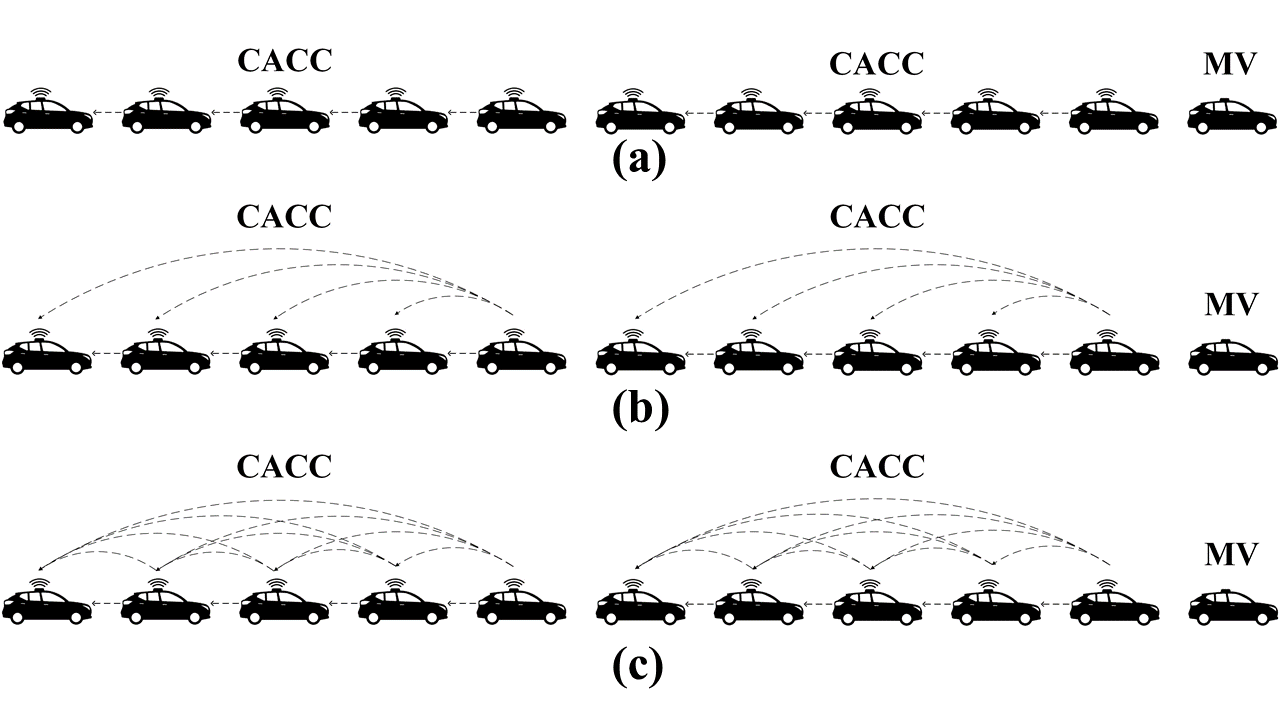
\includegraphics[width=9cm]{fig1.png}
  \caption{~Typical information flow topologies: (a) predecessor-following (PF), (b) predecessor-leader-following (PLF), (c) multiple-predecessor-leader-following (MPLF).}
  \label{Figure1}
\end{figure}


\subsection{Traffic Flow Configurations}

\begin{figure}
  \centering
  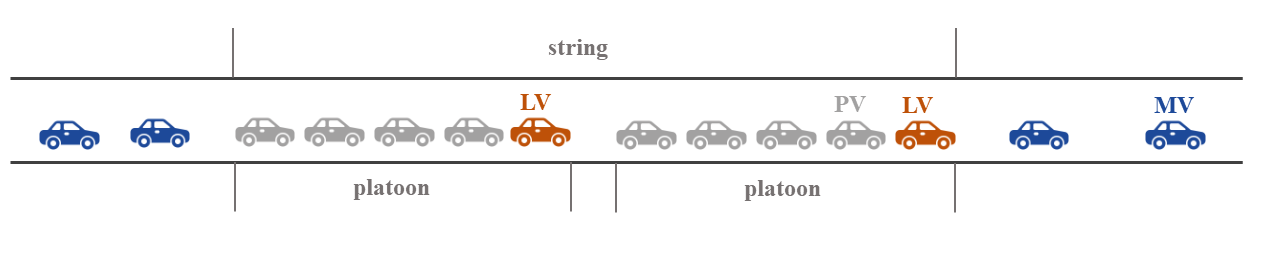
\includegraphics[width=9cm]{fig2.png}
  \caption{~The Traffic Flow Configurations.}
  \label{Figure2}
\end{figure}

As shown in Fig.~\ref{Figure2}, platoon management is expressed under the condition that when the CACC string reaches the maximum number of vehicles that C-V2X can maintain stable communication, the existing platoon is not included in the subsequent CACC, but a newly-formed platoon. The maximum platoon size $S$ is limited by the maximum C-V2X communication bandwidth. Assume that the traffic flow includes three types of vehicles:


\begin{enumerate}
  \item \emph{MV} (Manual Vehicle) - regular cars maneuvered by humans;
  \item \emph{LV} (Leader Vehicle) - the leader vehicle of the platoon following an MV and its control mechanism is similar to ACC, which cannot obtain the gain of communication and only sends information to its following vehicles \citep{zheng2014influence};
  \item \emph{PV} (Platoon Vehicle) - the vehicle inside the platoon which receives information from both preceding vehicle and platoon leader vehicle; The information flow topology of this type of vehicle can be Predecessor-Following (PF), Predecessor-Leader Following (PLF), or multiple-predecessor-leader-following (MPLF) \citep{zheng2014influence}.
\end{enumerate}


This paper mainly analyzes the linear string stability of the CACC platoon and designs controllers under different IFTs. The specific platoon consists of a \emph{LV} and $S-1$ \emph{PV}s.

\section{Car-Following Model}
\label{Section 3}
\subsection{Car-Following Model}

In previous studies, there are generally two methods for modeling the car-following behavior of CACCs: 1) simulating based on modified traffic flow models \citep{farah2014cooperative,yu2015effects,li2015stability}, and 2) modeling based on vehicle models or controllers with experimental data \citep{fernandes2014multiplatooning,milanes2014modeling,milanes2013cooperative}. From the practical application perspective, there is no doubt that the data model based on field tests is closer to the actual situation. However, the high cost and safety risks of CACC field tests make it impractical to conduct large-scale field tests at present. Furthermore, using the fitted model to model the longitudinal behavior abstracts the internal mechanism of the controller, which is not conducive to the design of the CACC controller. In summary, this paper is mainly based on simulations instead of field tests. Moreover, a general form is adopted to simulate longitudinal car-following for the sake of universality and suitability.

\subsubsection{ACC Model}
As for ACC, due to the lack of communication modules, the car-following decision is completely based on its perception of the surrounding situation. According to the existing models used to describe the ACC car-following behavior, its decision-making mainly depends on its velocity, the spacing from the preceding vehicle, and the velocity difference with the preceding vehicle. Therefore, the general form used in this paper is as follows:
\begin{equation}
  \frac{d v_{n}(t)}{d t}=g_{n}\left(v_{n}(t-\tau), s_{n}(t-\tau), \Delta v_{n}(t-\tau)\right),
  \label{Eq1}
\end{equation}
where $g_n (t)$ is the acceleration; $\tau$ is the time delay of decision; $v_n (t)$ is the velocity; $\Delta v_n (t)$ is the velocity difference between the subject vehicle and the preceding vehicle; $s_n (t)$ is the spacing between the subject vehicle and its predecessor.

\subsubsection{CACC Model}

The CACC system, which incorporates a V2V communication module, is an enhancement of the ACC system. With the gain of communication for system stability, CACC can maintain smaller time gaps and perception delays, thereby improving traffic capacity and safety. According to the definition of CACC \citep{dey2015review}, the essential component is the communication module, which receives information from other CACC-enabled vehicles through VANET. Instead of simply using a smaller time gap to represent communication gain, an additional component has been added to the longitudinal model to describe the communication gain, meaning the information obtained from preceding vehicles via the communication module.


For PF, the transmitted information only includes the position, velocity, and acceleration of the preceding vehicle, so the general form used to simulate CACCs based on PF is as follows:
\begin{equation}
  \begin{aligned}
    \frac{d v_{n}(t)}{d t}= & g_{n}\left(v_{n}(t-\tau), s_{n}(t-\tau), \Delta v_{n}(t-\tau)\right)                      \\
                            & +\gamma_{p} g_{n-1}\left(v_{n-1}(t-\tau), s_{n-1}(t-\tau), \Delta v_{n-1}(t-\tau)\right),
  \end{aligned}
  \label{Eq2}
\end{equation}
where $g_n (*)$ denotes the acceleration based on the general form of ACC system; $\gamma_p$ is the weighting coefficient of communication gain from the preceding vehicle.


As for PLF, the transmitted information includes the position, velocity, and acceleration of the platoon leader vehicle and preceding vehicle. In this case, the general form used to simulate CACCs based on PLF is as follows:
\begin{equation}
  \begin{aligned}
    \frac{d v_{n}(t)}{d t}= & g_{n}\left(v_{n}(t-\tau), s_{n}(t-\tau), \Delta v_{n}(t-\tau)\right)                     \\
                            & +\gamma_{p} g_{n-1}\left(v_{n-1}(t-\tau), s_{n-1}(t-\tau), \Delta v_{n-1}(t-\tau)\right) \\
                            & +\gamma_{l} g_{1}\left(v_{1}(t-\tau), s_{1}(t-\tau), \Delta v_{1}(t-\tau)\right),
  \end{aligned}
  \label{Eq3}
\end{equation}
where, $\gamma_p$ is the weighting coefficient of communication gain from preceding vehicle; $\gamma_l$ is the weighting coefficient of communication gain from leader vehicle.

When the problem comes to MPLF, the transmitted information includes the position, velocity, and acceleration of the platoon leader and all the preceding vehicles in the platoon. Therefore, the expression of the general form for CACC based on MPLF is as follows:
\begin{equation}
  \begin{aligned}
    \frac{d v_{n}(t)}{d t}  = & g_{n} \left(v_{n}(t-\tau), s_{n}(t-\tau), \Delta v_{n}(t-\tau)\right)                                      \\
                              & +\sum_{k=1}^{n-1} \gamma_{k} g_{n-k}\left(v_{n-k}(t-\tau), s_{n-k}(t-\tau), \Delta v_{n-k}(t-\tau)\right),
  \end{aligned}
  \label{Eq4}
\end{equation}
where $\gamma_1=\gamma_2=\cdots	=\gamma_{n-1}$ represent the information communicated from leader and preceding vehicle has identical importance.

\subsection{{Perception delays}}

Different types of vehicles have various reaction delays in the process of obtaining information about the surrounding environment \citep{ngoduy2013analytical,yao2021linear}. It is worth noting that reaction delays in this paper refer to the delays of this type. Based on existing research and difference of perceived variables, we can divide the reaction delay into two parts: the reaction delay to the car-following gap $\tau_n^s$, and the reaction delay to the velocity difference $\tau_n^{\Delta v}$, where the reaction delay to vehicle velocity is due to the driver is focusing on the velocity of the vehicle all the time.

\begin{enumerate}
  \item \emph{MVs}: Since the reaction performance of MVs cannot benefit from the intelligent and connected environment during driving, their time delays do not change. Set the time delay value to:
        $\tau_{mv}^{s}$=0.4s, $\tau_{mv}^{\Delta v}$=0.4s;
  \item \emph{LVs}: Since LVs are controlled by the Adaptive Cruise Control system, there is no response time delay and decision time delay. However, it cannot communicate, and sensing the state of the vehicle ahead depends entirely on the onboard radar, which has an inevitable sensing delay. Set the delay value to: $\tau_{lv}^{s}$=0.2s, $\tau_{lv}^{\Delta v}$=0.2s;
  \item \emph{PVs}: Due to the intelligent and connected environment, PVs receive the information of the vehicle ahead through the onboard communication system, so its communication delay is almost negligible compared with other delays. Set the delay value to: $\tau_{pv}^{s}$=0s, $\tau_{pv}^{\Delta v}$=0s.
\end{enumerate}


\section{Linear Stability analysis of CACC platoon controller}
\label{Section 4}
In this section, since most of the disturbances faced by drivers during normal driving are tiny disturbances, we apply the linear stability method for the extended intelligent driver model described by Equation (\ref{Eq2})-(\ref{Eq4}) to obtain the stability criterion of the CACC platoon \citep{jin2014dynamics,sun2018stability}. Since CACCs based on different IFTs use a similar general model, they can apply the framework of linear stability analysis to obtain the corresponding stability criteria in a similar process. Hence, the following content only takes CACC based on PLF as an example.
In the equilibrium state, the vehicle velocity in the traffic flow is equal to the equilibrium state velocity $v_e$; the velocity difference between adjacent vehicles is zero; the car-following gap between the vehicles maintains the desired gap $s_n^e$; and the acceleration of the vehicle is zero. So, we can get:
\begin{equation}
  \left\{\begin{array}{l}
    v_{n}=v_{n}^{e}, \\
    s_{n}=s_{n}^{e}, \\
    \Delta v_{n}=0,  \\
    g_{n}\left(v_{n}^{e}, s_{n}^{e}, 0\right)=0.
  \end{array}\right.
  \label{Eq5}
\end{equation}

Now let $\delta v_n$ and $\delta s_n$ denote the small deviation of the velocity and gap around the equilibrium state. The state after the disturbance can be expressed as:
\begin{equation}
  \left\{\begin{array}{l}
    v_{n}=v_{n}^{e}+\delta v_{n}, \\
    s_{n}=s_{n}^{e}+\delta s_{n}, \\
    \Delta v_{n}=0+\Delta\left(\delta v_{n}\right).
  \end{array}\right.
  \label{Eq6}
\end{equation}

By introducing the multiple reaction delays into the:
\begin{equation}
  \begin{aligned}
    \frac{d \delta v_{n}(t)}{d t} & =g_{n}\left(v_{n}^{e}, s_{n}^{e}, 0\right)+g_{n}\left(v_{n}(t), s_{n}\left(t-\tau_{n}^{s}\right), \Delta v_{n}\left(t-\tau_{n}^{\Delta v}\right)\right) \\
                                  & +\gamma_{p} g_{n-1}\left(v_{n-1}(t), s_{n-1}\left(t-\tau_{n-1}^{s}\right), \Delta v_{n-1}\left(t-\tau_{n-1}^{\Delta v}\right)\right)                    \\
                                  & +\gamma_{l} g_{1}\left(v_{1}(t), s_{1}\left(t-\tau_{1}^{s}\right), \Delta v_{1}\left(t-\tau_{1}^{\Delta v}\right)\right).
  \end{aligned}
  \label{Eq7}
\end{equation}

Substituting Equation (\ref{Eq5}) and (\ref{Eq6}) into (\ref{Eq7}), the acceleration expression under small disturbance is as follows:
\begin{equation}
  \begin{aligned}
    \frac{d \delta v_{n}(t)}{d t}= & g_{n}^{v} \delta v_{n}(t)+g_{n}^{s} \delta s_{n}\left(t-\tau_{n}^{s}\right)-g_{n}^{\Delta v} \Delta\left(\delta v_{n}\left(t-\tau_{n}^{\Delta v}\right)\right)                          \\
                                   & +\gamma_{p}\left[g_{n-1}^{v} \delta v_{n-1}(t)+g_{n-1}^{s} \delta s_{n-1}\left(t-\tau_{n-1}^{s}\right)\right.                                                                           \\
                                   & \quad\left.-g_{n-1}^{\Delta v} \Delta\left(\delta v_{n-1}\left(t-\tau_{n-1}^{\Delta v}\right)\right)\right]                                                                             \\
                                   & +\gamma_{l}\left[g_{1}^{v} \delta v_{1}(t)+g_{1}^{s} \delta s_{1}\left(t-\tau_{1}^{s}\right)-g_{1}^{\Delta v} \Delta\left(\delta v_{1}\left(t-\tau_{1}^{\Delta v}\right)\right)\right],
  \end{aligned}
  \label{Eq8}
\end{equation}
\begin{equation}
  \frac{d \delta s_{n}(t)}{d t}=\delta v_{n-1}(t)-\delta v_{n}(t),
  \label{Eq9}
\end{equation}
where $g_{n}^{v}=\left.\frac{\partial g_{n}}{\partial v_{n}}\right|_{\left(v_{n}^{e}, s_{n}^{e}, 0\right)}$, $g_{n}^{s}=\left.\frac{\partial g_{n}}{\partial s_{n}}\right|_{\left(v_{n}^{e}, s_{n}^{e}, 0\right)}$, and $g_{n}^{\Delta v}=\left.\frac{\partial g_{n}}{\partial \Delta v_{n}}\right|_{\left(v_{n}^{e}, s_{n}^{e}, 0\right)}$ are the partial differential equations at the equilibrium state (where the velocity is equilibrium velocity $v_{n}^{e}$, the gap is the equilibrium gap $s_{n}^{e}$ and the velocity difference is zero) for velocity, gap, velocity difference, respectively. To obtain the characteristic equation under the disturbance, a reasonable form hypothesis for the disturbance must be proposed. Fortunately, the disturbance propagation can be translated into a vibration and diffusion problem on a one-dimensional discrete medium, where disturbance and vehicle platoon are defined as vibration and one-dimensional discrete medium, respectively. Based on the translation above, the form of disturbances can be given as Fourier-ansatz. Moreover, considering that the disturbance from the preceding vehicle is not equal to zero, the traditional Fourier-ansatz $\delta v_{n}(t)=\hat{v} e^{\lambda t}$ and $\delta s_{n}(t)=\hat{s} e^{\lambda t}$ are not applicable. Based on the superposition principle of linear system, Fourier-ansatz can evolve into $\delta v_{n}(t)=\hat{\mathrm{v}} e^{i n \varphi+\lambda t}$ and $\delta s_{n}(t)=\hat{\mathrm{s}} e^{i n \varphi+\lambda t}$ to represent the disturbance from the preceding vehicle, where $\hat{\mathrm{v}}$ and $\hat{\mathrm{s}}$ are constants independent of $n$ and $t$, $\lambda$ is the eigenvalues of disturbances, and $\varphi$ is the phase of the disturbance propagation. Based on the Fourier-ansatz and difference equation Equation (\ref{Eq9}), we can obtain:
\begin{equation}
  s_{n}=\frac{v_{n-1}(t)-v_{n}(t)}{\lambda}.
  \label{Eq10}
\end{equation}

Take Fourier-ansatz and Equation (\ref{Eq10}) into (\ref{Eq8}):
\begin{equation}
  \left\{\begin{array}{c}
    \lambda^{2}V_{n}=\psi_{n}+\gamma_{p} \psi_{n-1} e^{-i \varphi}+\gamma_{l} \psi_{1} e^{-i(n-1) \varphi}, \\
    \psi_{n}=\left(g_{n}^{s} e^{-\lambda \tau_{n}^{s}}-g_{n}^{\Delta v} e^{-\lambda_{n}^{\Delta v}}\right)\left(e^{-i \varphi}V_{n-1}-V_{n}\right)+g_{n}^{v} \lambda V_{n}.
  \end{array}\right.
  \label{Eq11}
\end{equation}

The reaction delay term is exponentially expanded to the second order, $e^{-\lambda \tau}=1-\lambda \tau+ ({\lambda \tau})^2/2$, and the third-order characteristic equation of $\lambda$ is obtained:
\begin{small}
  \begin{equation}
    \begin{aligned}
      \psi_{n}\!= & \!\left[A_{n} \lambda^{3}\!+\!B_{n} \lambda^{2}\!+\!C_{n} \lambda^{1}\!+\!D_{n} \lambda^{0}\right] V_{n}                   \\
                  & +\!\left[H_{n} \lambda^{3}\!+\!I_{n} \lambda^{2}\!+\!J_{n} \lambda^{1}\!+\!K_{n} \lambda^{0}\right] e^{-i \varphi}V_{n-1},
      \label{Eq12}
    \end{aligned}
  \end{equation}
\end{small}
where,
\begin{equation}
  \left\{\begin{array}{l}
    A_{n}=0.5 g_{n}^{\Delta v}\left(\tau_{n}^{\Delta v}\right)^{2},                                      \\
    B_{n}=-\left(g_{n}^{\Delta v} \tau_{n}^{\Delta v}+0.5 g_{n}^{s}\left(\tau_{n}^{s}\right)^{2}\right), \\
    C_{n}=g_{n}^{v}+g_{n}^{\Delta v}+g_{n}^{s} \tau_{n}^{s},                                             \\
    D_{n}=-g_{n}^{s},                                                                                    \\
    H_{n}=-0.5 g_{n}^{\Delta v}\left(\tau_{n}^{\Delta v}\right)^{2},                                     \\
    I_{n}=g_{n}^{\Delta v} \tau_{n}^{\Delta v}+0.5g_{n}^{s}\left(\tau_{n}^{s}\right)^{2},                \\
    J_{n}=-\left(g_{n}^{\Delta v}+g_{n}^{s} \tau_{n}^{s}\right),                                         \\
    K_{n}=g_{n}^{s}.
  \end{array}\right.
  \label{Eq13}
\end{equation}

Substitute Equation (\ref{Eq13}) into (\ref{Eq11}), the third-order characteristic equation of CACC platoon is as follows:
\begin{equation}
  \begin{aligned}
    \lambda^{2}V_{n}\! & =\!\left[A_{n} \lambda^{3}\!+\!B_{n} \lambda^{2}\!+\!C_{n} \lambda^{1}\!+\!D_{n} \lambda^{0}\right]V_{n}\!                       \\
                       & +\!\left[H_{n} \lambda^{3}\!+\!I_{n} \lambda^{2}\!+\!J_{n} \lambda^{1}\!+\!K_{n} \lambda^{0}\right] e^{-i \varphi} V_{n-1}       \\
                       & +\gamma_{p}\left[A_{n-1} \lambda^{3}+B_{n-1} \lambda^{2}+C_{n-1} \lambda^{1}+D_{n-1} \lambda^{0}\right] e^{-i \varphi} V_{n-1}   \\
                       & +\gamma_{p}\left[H_{n-1} \lambda^{3}+I_{n-1} \lambda^{2}+J_{n-1} \lambda^{1}+K_{n-1} \lambda^{0}\right] e^{-i 2 \varphi} V_{n-2} \\
                       & +\gamma_{l}\left[A_{1} \lambda^{3}+B_{1} \lambda^{2}+C_{1} \lambda^{1}+D_{1} \lambda^{0}\right] e^{-i(n-1) \varphi} V_{1}        \\
                       & +\gamma_{l}\left[H_{1} \lambda^{3}+I_{1} \lambda^{2}+J_{1} \lambda^{1}+K_{1} \lambda^{0}\right] e^{-i n \varphi}V_{0}.
  \end{aligned}
  \label{Eq14}
\end{equation}

To maintain linear string stability of CACC platoons, the solutions of the third-order characteristic equation $\lambda$ satisfy Re($\lambda$)$\leq$0. The zero solution $\varphi=0$,$\lambda_0=0$ of the real number domain that satisfies the conditions can be easily obtained to analyze the changing trend of $\lambda$ with $\varphi$. Suppose $\lambda$ is the power series solution: Among them, $\lambda_1$ and $\lambda_2$ are real coefficients. At the same time, expand $e^{-i \varphi N}$ to a second-order power series: $e^{-i \varphi N}=1-i \varphi N-\frac{N^{2} \varphi^{2}}{2}$. By introducing the periodic traffic scenario and solving the algebraic formula, we can get:
\begin{small}
  \begin{equation}
    \begin{aligned}
      \Gamma(\varphi) & =\left[C_{n}+J_{n}\right.\left.+\gamma_{p}\left(C_{n-1}+J_{n-1}\right)+\gamma_{l}\left(C_{1}+J_{1}\right)\right] \lambda_{1}       \\
                      & \!-\!\left[K_{n}\!+\!\gamma_{p}\left(D_{n-1}\!+\!2 K_{n-1}\right)\!+\!\gamma_{l}\left((n-1) D_{1}\!+\!n K_{1}\right)\right]\!=\!0,
    \end{aligned}
    \label{Eq15}
  \end{equation}
\end{small}
\begin{small}
  \begin{equation}
    \begin{aligned}
      \Gamma\left(\varphi^{2}\right) & =\left[C_{n}+J_{n}\right.\left.+\gamma_{p}\left(C_{n-1}+J_{n-1}\right)+\gamma_{l}\left(C_{1}+J_{1}\right)\right] \lambda_{2}                               \\
                                     & \!-\!\left[\left(B_{n}\!+\!I_{n}-1\right)\!+\!\gamma_{p}\left(B_{n-1}\!+\!I_{n-1}\right)\!+\!\gamma_{l}\left(B_{1}\!+\!I_{1}\right)\right] \lambda_{1}^{2} \\
                                     & \!+\!\left[J_{n}\!+\!\gamma_{p}\left(C_{n-1}\!+\!2 J_{n-1}\right)\!+\!\gamma_{l}\left((n-1) C_{1}\!+\!\mathrm{n} J_{1}\right)\right] \lambda_{1}           \\
                                     & -\left[0.5 K_{n}+\gamma_{p}\left(0.5 D_{n-1}+2 K_{n-1}\right)\right.                                                                                       \\
                                     & \quad\left.+\gamma_{l}\left(0.5(n-1)^{2} D_{1}+0.5 n^{2} K_{1}\right)\right]=0.
    \end{aligned}
    \label{Eq16}
  \end{equation}
\end{small}

The expression of $\lambda_1$ and $\lambda_2$ can be obtained by solving the Equation (\ref{Eq15}) and (\ref{Eq16}):
\begin{equation}
  \begin{gathered}
    \lambda_{1}=\frac{\left[K_{n}+\gamma_{p}\left(D_{n\!-\!1}+2 K_{n\!-\!1}\right)+\gamma_{l}\left((n\!-\!1) D_{1}+n K_{1}\right)\right]}{\left[C_{n}+J_{n}+\gamma_{p}\left(C_{n\!-\!1}+J_{n\!-\!1}\right)+\gamma_{l}\left(C_{1}+J_{1}\right)\right]} \\
    =\frac{g_{n}^{s}+\gamma_{p} g_{n\!-\!1}^{s}+\gamma_{l} g_{1}^{s}}{g_{n}^{v}+\gamma_{p} g_{n\!-\!1}^{v}+\gamma_{l} g_{1}^{v}},
  \end{gathered}
  \label{Eq17}
\end{equation}
\begin{equation}
  \begin{gathered}
    \begin{aligned}
                   & {\left[\left(B_{n}\!+\!I_{n}\!-\!1\right)\!+\!\gamma_{p}\left(B_{n\!-\!1}\!+\!I_{n\!-\!1}\right)\!+\!\gamma_{l}\left(B_{1}\!+\!I_{1}\right)\right] \lambda_{1}^{2}}                                                                                                                                  \\
                   & \!-\!\left[J_{n}\!+\!\gamma_{p}\left(C_{n\!-\!1}\!+\!2 J_{n\!-\!1}\right)\!+\!\gamma_{l}\left(\left(n\!-\!1\right) C_{1}\!+\!n J_{1}\right)\right] \lambda_{1}                                                                                                                                       \\
      \lambda_{2}= & \frac{\!+\!\left[0.5 K_{n}\!+\!\gamma_{p}\left(0.5 D_{n\!-\!1}\!+\!2 K_{n\!-\!1}\right)\!+\!\gamma_{l}\left(0.5(n\!-\!1)^{2} D_{1}\!+\!0.5n^{2} K_{1}\right)\right]}{\left[C_{n}\!+\!J_{n}\!+\!\gamma_{p}\left(C_{n\!-\!1}\!+\!J_{n\!-\!1}\right)\!+\!\gamma_{l}\left(C_{1}\!+\!J_{1}\right)\right]} \\
      \\
    \end{aligned}
    \\
    \begin{aligned}
        & \!-\!\lambda_{1}^{2}\!+\!\left[\left(g_{n}^{\Delta v}\!+\!g_{n}^{s} \tau_{n}^{s}\right)\!+\!\gamma_{p}\left(g_{n\!-\!1}^{\Delta v}\!+\!g_{n\!-\!1}^{s} \tau_{n\!-\!1}^{s}\!-\!g_{n\!-\!1}^{v}\right)\right. \\
        & \left.+\gamma_{l}\left(g_{1}^{\Delta v}\!+\!g_{1}^{s} \tau_{1}^{s}\!-\!(n\!-\!1) g_{1}^{v}\right)\right] \lambda_{1}                                                                                        \\
      = & \frac{\!+\!\left[0.5 g_{n}^{s}\!+\!\gamma_{p} 1.5 g_{n\!-\!1}^{s}\!+\!0.5(2 n\!-\!1) \gamma_{1} g_{1}^{s}\right]}{g_{n}^{v}\!+\!\gamma_{p} g_{n\!-\!1}^{v}\!+\!\gamma_{l} g_{1}^{v}}.
    \end{aligned}
  \end{gathered}
  \label{Eq18}
\end{equation}




From the conditions of $g_n^s>0$,$g_n^v<0$, it can be known that $\lambda_1$ always satisfies the stability condition, then the criterion of string stability becomes $\lambda_2\leq0$:
\begin{equation}
  \begin{gathered}
    \begin{aligned}
       & \!-\!\lambda_{1}^{2}\!+\!\left[\left(g_{n}^{\Delta v}\!+\!g_{n}^{s} \tau_{n}^{s}\right)\!+\!\gamma_{p}\left(g_{n\!-\!1}^{\Delta v}\!+\!g_{n\!-\!1}^{s} \tau_{n\!-\!1}^{s}\!-\!g_{n\!-\!1}^{v}\right)\right. \\
       & \left.+\gamma_{l}\left(g_{1}^{\Delta v}\!+\!g_{1}^{s} \tau_{1}^{s}\!-\!(n\!-\!1) g_{1}^{v}\right)\right] \lambda_{1}                                                                                        \\
       & \frac{+\left[0.5 g_{n}^{s}\!+\!\gamma_{p} 1.5 g_{n\!-\!1}^{s}\!+\!0.5(2 n\!-\!1) \gamma_{1} g_{1}^{s}\right]}{g_{n}^{v}\!+\!\gamma_{p} g_{n\!-\!1}^{v}\!+\!\gamma_{l} g_{1}^{v}} \leq 0.
    \end{aligned}
  \end{gathered}
  \label{Eq19}
\end{equation}


For the CACC platoon, $g_n^s=g_{n-1}^s=g_1^s$, $g_n^{\Delta v}=g_{n-1}^{\Delta v}=g_1^{\Delta v}$, $g_n^v=g_{n-1}^v=g_1^v$ should be satisfied, which means Equation (\ref{Eq19}) can be simplified as:
\begin{small}
  \begin{equation}
    \begin{aligned}
      F_{PLF} & =\left[g_{n}^{\Delta v}\left(1\!+\!\gamma_{p}\!+\!\gamma_{l}\right)\!+\!g_{n}^{s}\left(\tau_{n}^{s}\!+\!\gamma_{p} \tau_{n\!-\!1}^{s}\!+\!\gamma_{l} \tau_{1}^{s}\right)\!+\!\left(\gamma_{p}\!+\!(n\!\!-\!\!1) \gamma_{l}\right) g_{n}^{v}\right] g_{n}^{v} \\
              & \quad+\!\left(g_{n}^{v}\right)^{2}\left[0.5\!+\!1.5 \gamma_{p}\!+\!0.5(2 n\!-\!1) \gamma_{l}\right]\!\!-\!g_{n}^{s}\!                                                                                                                                        \\
              & =g_{n}^{v} g_{n}^{s}\left(\tau_{n}^{s}\!+\!\gamma_{p} \tau_{n\!-\!1}^{s}\!+\!\gamma_{l} \tau_{1}^{s}\right)\!+\!g_{n}^{v} g_{n}^{\Delta v}\left(1\!+\!\gamma_{p}\!+\!\gamma_{l}\right)                                                                       \\
              & \quad \!+\!0.5\left(g_{n}^{v}\right)^{2}\left(1\!+\!\gamma_{p}\!+\!\gamma_{l}\right)\!-\!g_{n}^{s}                                                                                                                                                           \\
              & \geq 0.
    \end{aligned}
    \label{Eq70}
  \end{equation}
\end{small}

For the sake of brevity of the paper, the specific stability criterion derivation process is omitted. Applying the above similar linear stability analysis method, the corresponding string stability criterions of PF and MPLF are as follows:
\begin{equation}
  \begin{aligned}
    F_{PF}
     & = g_{n}^{v} g_{n}^{s}\left(\tau_{n}^{s}\!+\!\gamma_{p} \tau_{n\!-\!1}^{s}\right)\!+\!g_{n}^{v} g_{n}^{\Delta v}\left(1\!+\!\gamma_{p}\right)\! \\
     & \quad +\!0.5\left(g_{n}^{v}\right)^{2}\left(1\!+\!\gamma_{p}\right)\!-\!g_{n}^{s} \geq 0,
  \end{aligned}
  \label{Eq21}
\end{equation}
\begin{equation}
  \begin{aligned}
    F_{MPLF}= & g_{n}^{v} g_{n}^{s}\left(\tau_{n}^{s}\!+\!\sum_{k=1}^{n\!-\!1} \gamma_{k} \tau_{n\!-\!k}^{s}\right)\!+\!g_{n}^{v} g_{n}^{\Delta v}\left(1\!+\!\sum_{k=1}^{n\!-\!1} \gamma_{k}\right) \\
              & \quad\!+\!0.5\left(g_{n}^{v}\right)^{2}\left(1\!+\!\sum_{k=1}^{n\!-\!1} \gamma_{k}\right)\!-\!g_{n}^{s} \geq 0.
  \end{aligned}
  \label{Eq22}
\end{equation}


Moreover, based on Equation (\ref{Eq70})-(\ref{Eq22}), a corresponding head-to-tail string stability criterion has also been proposed for three different IFTs \citep{ngoduy2013analytical,2009Heterogeneity}, since we are comparing the impact of different IFTs applied to CACC platoons. The expression is as follows:
\begin{equation}
  \begin{aligned}
    Q_{PF}= & \left[ g_{n}^{v} g_{n}^{s} \tau_{n}^{s} \!+\!g_{n}^{v} g_{n}^{\Delta v}+0.5\left(g_{n}^{v}\right)^{2}\!-\!g_{n}^{s} \right]                                                      \\
            & +\left(S\!-\!1\right) \left[g_{n}^{v} g_{n}^{s}\left(\tau_{n}^{s}\!+\!\gamma_{p} \tau_{n\!-\!1}^{s}\right)\!+\!g_{n}^{v} g_{n}^{\Delta v}\left(1\!+\!\gamma_{p}\right)\! \right. \\
            & \left. +0.5\left(g_{n}^{v}\right)^{2}\left(1\!+\!\gamma_{p}\right)\!-\!g_{n}^{s}\right]                                                                                          \\
            & \geq 0,
  \end{aligned}
  \label{Eq71}
\end{equation}
\begin{equation}
  \begin{aligned}
    Q_{PLF}= & \left[ g_{n}^{v} g_{n}^{s} \tau_{n}^{s} \!+\!g_{n}^{v} g_{n}^{\Delta v}+0.5\left(g_{n}^{v}\right)^{2}\!-\!g_{n}^{s} \right]                                                                                              \\
             & +\left(S\!-\!1\right)\left[g_{n}^{v} g_{n}^{s}\left(\tau_{n}^{s}\!+\!\gamma_{p} \tau_{n\!-\!1}^{s}\!+\!\gamma_{l} \tau_{1}^{s}\right)\!+\!g_{n}^{v} g_{n}^{\Delta v}\left(1\!+\!\gamma_{p}\!+\!\gamma_{l}\right) \right. \\
             & \left.+0.5\left(g_{n}^{v}\right)^{2}\left(1\!+\!\gamma_{p}\!+\!\gamma_{l}\right)\!-\!g_{n}^{s} \right]                                                                                                                   \\
             & \geq 0,
  \end{aligned}
  \label{Eq72}
\end{equation}
\begin{equation}
  \begin{aligned}
    Q_{MPLF}= & \left[ g_{n}^{v} g_{n}^{s} \tau_{n}^{s} \!+\!g_{n}^{v} g_{n}^{\Delta v}+0.5\left(g_{n}^{v}\right)^{2}\!-\!g_{n}^{s} \right]                                                                                       \\
              & +\sum_{n=2}^{S} \left[g_{n}^{v} g_{n}^{s}\left(\tau_{n}^{s}\!+\!\sum_{k=1}^{n\!-\!1} \gamma_{k} \tau_{n\!-\!k}^{s}\right)\!+\!g_{n}^{v} g_{n}^{\Delta v}\left(1\!+\!\sum_{k=1}^{n\!-\!1} \gamma_{k}\right)\right. \\
              & +\left.0.5\left(g_{n}^{v}\right)^{2}\left(1\!+\!\sum_{k=1}^{n\!-\!1} \gamma_{k}\right)\!-\!g_{n}^{s} \right]                                                                                                      \\
              & \geq 0.
  \end{aligned}
  \label{Eq73}
\end{equation}


\section{Comparisons between different IFTs}
\label{Section 5}
In order to explore the differences of different IFTs in stability region, robustness, safety, and emission, several numerical analyses and simulations were adopted in this section. For the stability region, based on the stability criterion of the CACC platoon controller in Equation (\ref{Eq70})-(\ref{Eq22}) obtained in Section~\ref{Section 4}, numerical analysis on the stability region related to desire time gap and velocity, and a comparison with the traditional ACC controller is conducted. The corresponding simulation verification is carried out under specific parameters. Moreover, we explored the difference of stability region under different controller designs for platoon CACCs, including PF-based, PLF-based, and MPLF-based. As for robustness, safety, and emission, which are difficult to reflect in the numerical analysis. Several related indicators in previous research were proposed to evaluate each aspect of different IFTs. Furthermore, numerical simulations were carried out for each aspect to make comparisons between different IFTs.


To conduct a specific comparative analysis of the differences between different IFTs, a specific model needs to be selected to represent the general form used above. The Intelligent Driver Model (IDM) is chosen for the following reasons. In addition, the general model can be represented by any model that can be used as the ACC control strategy. Firstly, the IDM, having only six parameters with concrete meanings, has been proven to precisely model car-following behaviors. Secondly, many studies used the IDM to model ACC and CACC vehicles \citep{chang2020analysis,li2017evaluation}, which also indicates the ability of the model to reflect operations of driving-assistant systems. The model is expressed as:
\begin{equation}
  g_{n}(t)=A\left[1-\left(\frac{v_{n}(t)}{v_{f}}\right)^{\delta}-\left(\frac{s_{0}+T_{n} v_{n}(t)+\frac{v_{n}(t) \Delta v_{n}(t)}{2 \sqrt{A b}}}{s_{n}(t)-l_{n}}\right)^{2}\right],
  \label{Eq23}
\end{equation}
where $g_n (t)$ is the acceleration; A denotes the maximum desired acceleration; $v_n (t)$ is the velocity; $v_f$ is the free-flow velocity; $\delta$ is the acceleration component ($\delta>0$); $s_0$ is the minimum safety distance; $T_n$ is the safety time headway; $\Delta v_n (t)$ is the velocity difference between the subject vehicle and the preceding vehicle; $b_i$ is the absolute maximum desired deceleration; $s_n (t)$ is the spacing between the preceding and the subject vehicle; and $l_n$ is the length of the vehicle. The parameters are shown in Table.\ref{Table1} \citep{kesting2008adaptive,kesting2007jam}, which are based on previous studies.

Moreover, the corresponding stability conditions under the IDM can be derived by substituting the partial differential equations of Equation (\ref{Eq23}): ${g_{IDM}^v =  - \frac{{4A{v^3}}}{{v_f^4}} - \frac{{2A{T_n}\left[ {1 - {{\left( {v/{v_f}} \right)}^4}} \right]}}{{{s^0} + v{T_n}}}}$, ${g_{IDM}^{\Delta v} = \sqrt {\frac{A}{b}} \frac{{v\left[ {1 - {{\left( {v/{v_f}} \right)}^4}} \right]}}{{{s^0} + v{T_n}}}}$, and ${g_{IDM}^s = 2A\frac{{{{\left[ {1 - {{\left( {v/{v_f}} \right)}^4}} \right]}^{\frac{3}{2}}}}}{{{s^0} + v{T_n}}}}$ into Equation (\ref{Eq71})-(\ref{Eq73}).

\begin{table}
  \centering
  \setlength{\abovecaptionskip}{0pt}
  \setlength{\belowcaptionskip}{10pt}%设置标题与表格的距离
  \caption{Parameters chosen for IDM.}
  \resizebox{0.5\textwidth}{!}{
    {\begin{tabular}{lcccccc} \toprule
          Parameter & \text A & $v_{f}$ & $\delta$ & $s_{0}$ & $b$ & $l$ \\ \midrule Value & $1\mathrm{~m}/\mathrm{s}^{2}$ & $33.3\mathrm{~m}/\mathrm{s}$ & 4 & $2\mathrm{~m}$  & $2\mathrm{~m}/\mathrm{s}^{2}$ & $5\mathrm{~m}$ \\ \bottomrule
        \end{tabular}}
  }
  \label{Table1}
\end{table}

\subsection{Simulation scenario}
\label{Section 5.1}
According to many existing studies \citep{gong2016constrained,li2014stop}, using traffic oscillation scenarios to compare the performance of different vehicle types is highly effective. Therefore, we continue to use this method for evaluating the performance of different IFTs on stability region, robustness, safety, and emission. The simulation scenario is as follows:

\textit{CACC platoon composition}: The simulation platoon includes an MV as the leader vehicle and five CACCs (the maximum platoon size S is assumed to be 5). The CACC following the MV degenerates to ACC, and other vehicles use the car-following model with general form as the longitudinal control model.

\textit{Simulation scheme}: At first, all vehicles maintain the same initial velocity and the desire time gap. In order to simulate most traffic scenarios, the disturbance is applied to the leader vehicle. Besides, the most common three disturbances are adopted, including:

\begin{enumerate}
  % \item \textit{Type \uppercase\expandafter{\romannumeral1} Traffic oscillation}: The acceleration of leader vehicle MV shows a sine wave with a period of 9s and a value of 0.7 $m/s^2$ in 5s$-$41s and the initial velocity is 10 $m/s^2$.
  % \item \textit{Type \uppercase\expandafter{\romannumeral2} equilibrium state}: The acceleration of leader vehicle MV remains at 0 and receives a small disturbance with a value of 0.7 $m/s^2$ in 1s at 20s and another disturban with a value of -0.4 $m/s^2$ in 1s at 40s.
  % \item \textit{Type \uppercase\expandafter{\romannumeral3} Stop and go}: The acceleration of leader vehicle MV  is the same as the \textit{Type \uppercase\expandafter{\romannumeral1}} but the initial velocity is 0 $m/s^2$.
  % \end{enumerate}
  \item \textit{Type \uppercase\expandafter{\romannumeral1} Sine disturbance}: The acceleration of leader vehicle MV shows a sine wave with a period of 9s and a magnitude of 0.16 $m/s^2$ in 5s$-$41s.
  \item \textit{Type \uppercase\expandafter{\romannumeral2} Custom disturbance}: The leader vehicle suddenly accelerates to 11.8m/s in 5s and keeps the velocity for 15s. The leader vehicle then decelerates to 8.2m/s and accelerates to 10m/s, while the following vehicles respond to this traffic oscillation scenario.
  \item \textit{Type \uppercase\expandafter{\romannumeral3} Impulse disturbance}: The form of disturbance is that the acceleration of the leader vehicle suddenly rose to 0.9 $m/s^2$ and -0.9 $m/s^2$ at 4s and 40s, respectively.
\end{enumerate}

The specific speed and acceleration curve figures of the leader vehicle under different disturbances are shown in Fig.~\ref{Figure5.2}. Moreover, each simulation for evaluating indicators is conducted ten times to avoid random error.

\begin{figure}
  \centering
  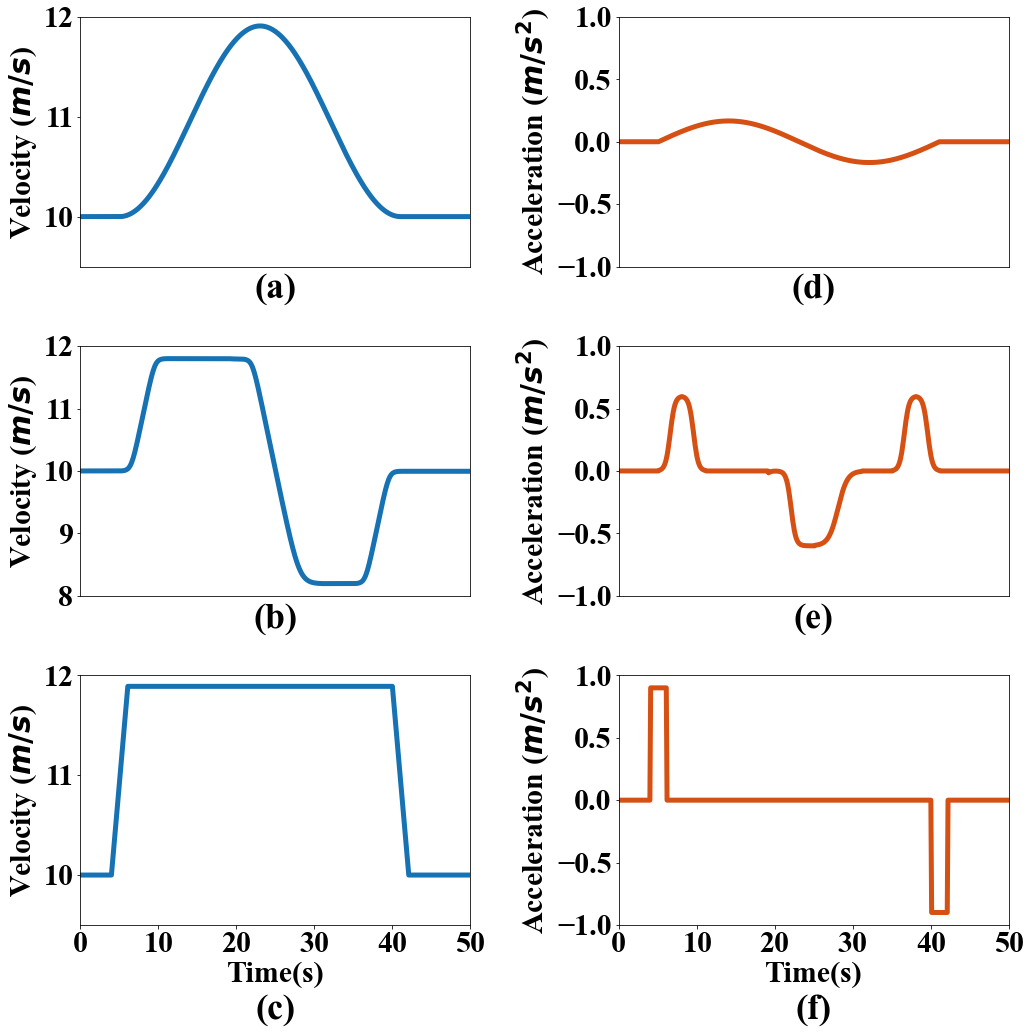
\includegraphics[width=9cm]{fig_S5.2.png}
  \caption{~The specific speed and acceleration curve figures of the leader vehicle under different disturbances. (a)-(c) the speed curve of {Type \uppercase\expandafter{\romannumeral1}}, {Type \uppercase\expandafter{\romannumeral2}}, and {Type \uppercase\expandafter{\romannumeral3}}; (d)-(f) the acceleration curve of {Type \uppercase\expandafter{\romannumeral1}}, {Type \uppercase\expandafter{\romannumeral2}}, and {Type \uppercase\expandafter{\romannumeral3}}}
  \label{Figure5.2}
\end{figure}


\subsection{Comparison of stability region}
\label{Section 5.2}
As an essential basis for the design of a controller, string stability must be ensured to avoid the disturbance from the upstream being amplified in the downstream traffic flow. So, the first item of comparison is the stability region of different IFTs.

\subsubsection{Margin stable curves of different IFTs}
\label{Section 5.2.1}
The basic principle of controller design is that a controller can keep string stable, so it is necessary to compare the margin stable curves of the three IFTs that can keep the string stable to get the margin stable time gap directly related to the traffic capacity.

Assuming the information from the leader and preceding vehicle is of equal importance, the $\gamma_p$ is set equal to $\gamma_l$ in this study. In addition, the weighting coefficient of communication gain of different IFTs is set to 0.3 to make them comparable. Based on the head-to-tail string stability criterion of different IFTs in Equation (\ref{Eq71})-(\ref{Eq73}), the heatmaps in the control space (velocity-desire time gap) are expressed in Fig.~\ref{Figure3}, and the black curve in each subfigure represents the margin stable curve. When the traffic flow environment and desire time gap setting is above the margin stable curve, it is string stable at equilibrium state, while the opposite represents the unstable traffic flow.

\begin{figure}
  \centering
  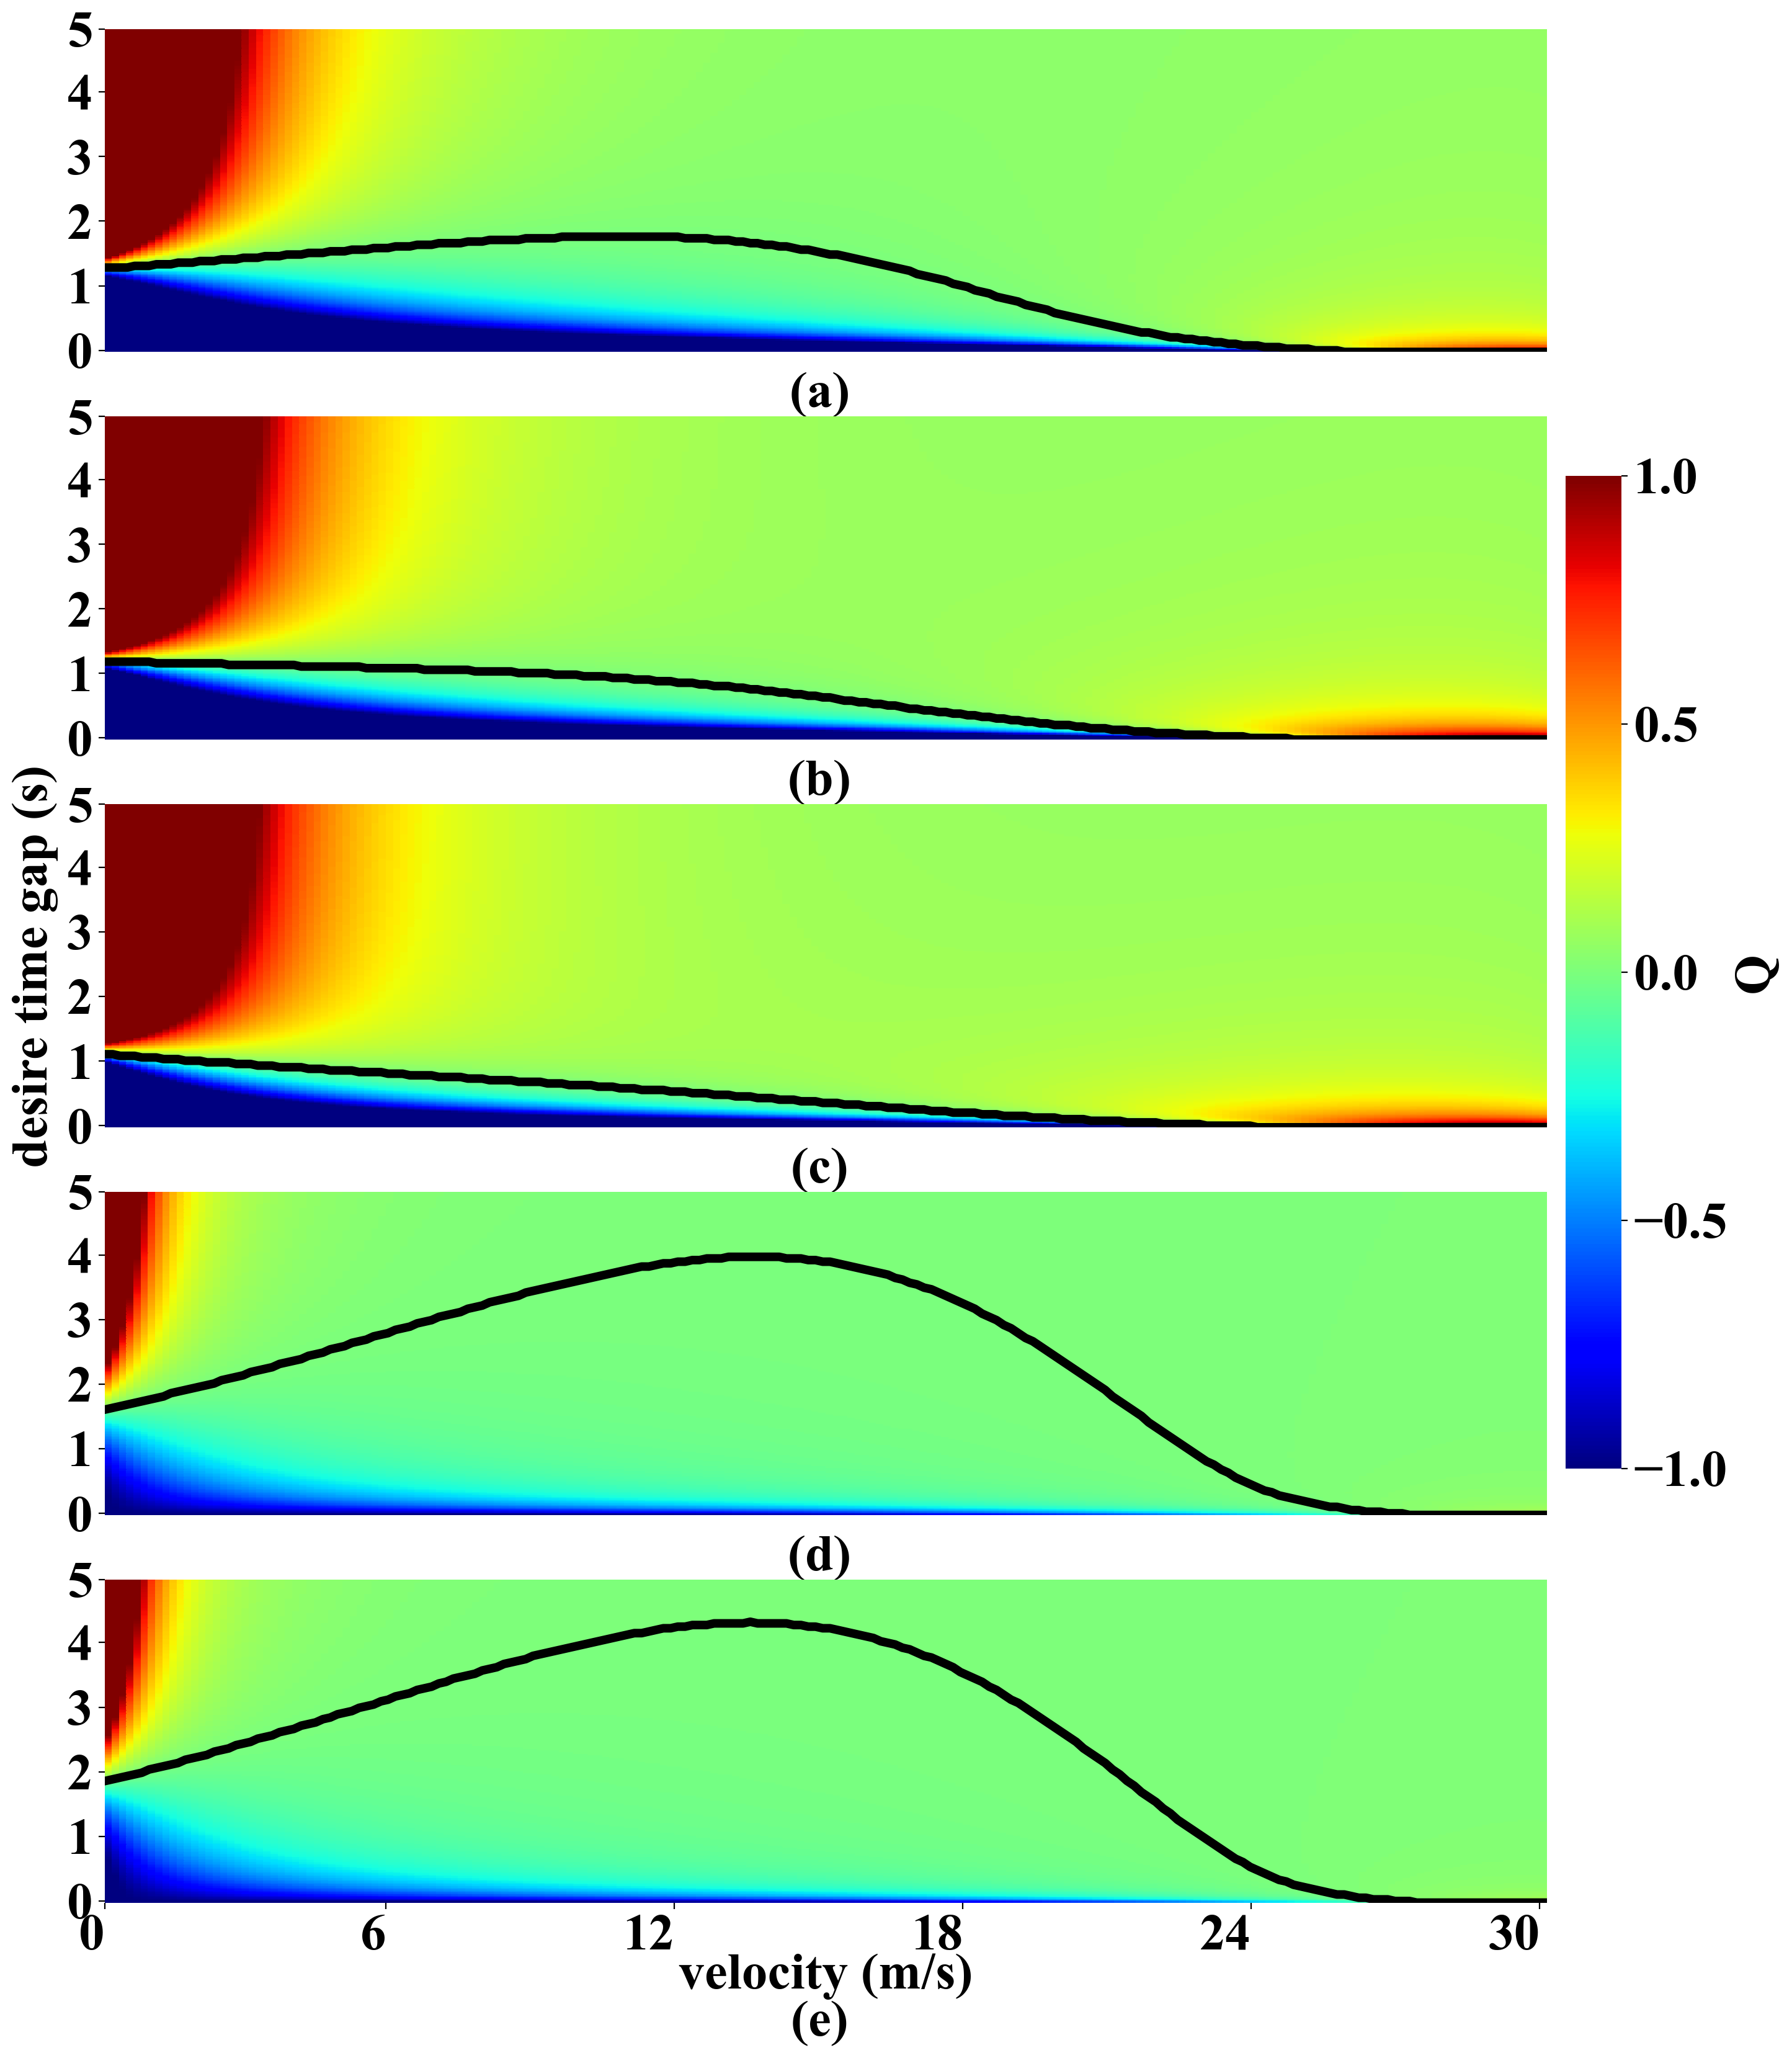
\includegraphics[width=9cm]{fig3.png}
  \caption{~The heatmaps in the velocity-desire time gap of different IFTs. (a) the case of PF; (b) the case of PLF; (c) the case of MPLF; (d) the case of ACC; (e) the case of MV.}
  \label{Figure3}
\end{figure}

Firstly, we focused on the head-to-tail string stability of different IFTs in the control space (velocity-desire time gap). It can be quickly noticed that there is a significant unstable peak in the cases of PF, ACC, and MV. Furthermore, this peak means that the head-to-tail string stability deteriorates over a specific velocity interval, adversely affecting traffic flow. Moreover, the head-to-tail string stability is sensitive to the desire time gap under low velocity but is insensitive under high velocity. In addition, all subfigures show the tendency that the margin stable curve is close to 0s under high velocity, which may be due to head-to-tail string stability being easier to maintain when the velocity is increased. From another perspective, both the heatmaps and margin stable curves of ACC and MV are similar, which is consistent with the conclusions reached in other studies.


Secondly, the difference between (a), (b), and (c) is worth noticing. It can be seen from Fig.~\ref{Figure3} that the margin stable curves of ACC and IDM are of distinct orders of magnitude compared with those of PF, PLF, and MPLF under different parameter settings, which means the adoption of CACC can significantly improve the traffic capacity by reducing desire time gap. For the CACC platoon controllers, it can be found that the margin stable curves are significantly lower than the ACC curve and are lower as parameters increase, which means obtaining the information from the preceding vehicle via communication can significantly improve the long-wave stability of traffic flow. Moreover, the curve of PF has a significantly unstable peak which is similar to the curves of ACC and MV. In contrast, the curves of PLF and MPLF can efficiently suppress the appearance of this peak under similar parameter settings to maintain a lower desire time gap in the entire velocity range. In addition, the curve of PLF is significantly lower than the curve of PF, and the critical desire time gap is only $39.53\%$ of PF when velocity = $10m/s$. This indicates that the controller based on PLF and MPLF can significantly improve traffic flow stability compared with PF on enhancing traffic flow capacity and safety. As for the difference between the margin stable curves of PLF and MPLF, the curve of MPLF is lower than the curve of PLF, and the reduced proportion is 41.18\% when velocity = $10m/s$, which means that obtaining more information from the further preceding vehicles can improve the stability of traffic flow. However, the reduced proportion of MPLF in the entire velocity range is only 30.41\%.

Based on the above analysis, one conclusion can be drawn that MPLF can keep the desire time gap to a minimum without losing head-to-tailing stability among IFTs. Both PLF and MPLF are able to suppress deterioration of stability due to increased velocity, whereas PF is not.



\subsubsection{Margin stable curves of IFTs under different parameters}
\label{Section 5.2.2}
In Section~\ref{Section 5.2.1}, the weighting coefficient of communication gain of different IFTs is all set to 0.3 to make them comparable. However, another problem arises with setting the weighting coefficient of communication gain. For this purpose, the numerical analysis of the different parameter settings is also carried out. Derived from Equation (\ref{Eq71})-(\ref{Eq73}), the heatmaps in the control space (velocity-desire time gap) under different parameter settings are expressed in Fig.~\ref{Figure4}, and the black curve in each subfigure represents the margin stable curve.

\begin{figure}
  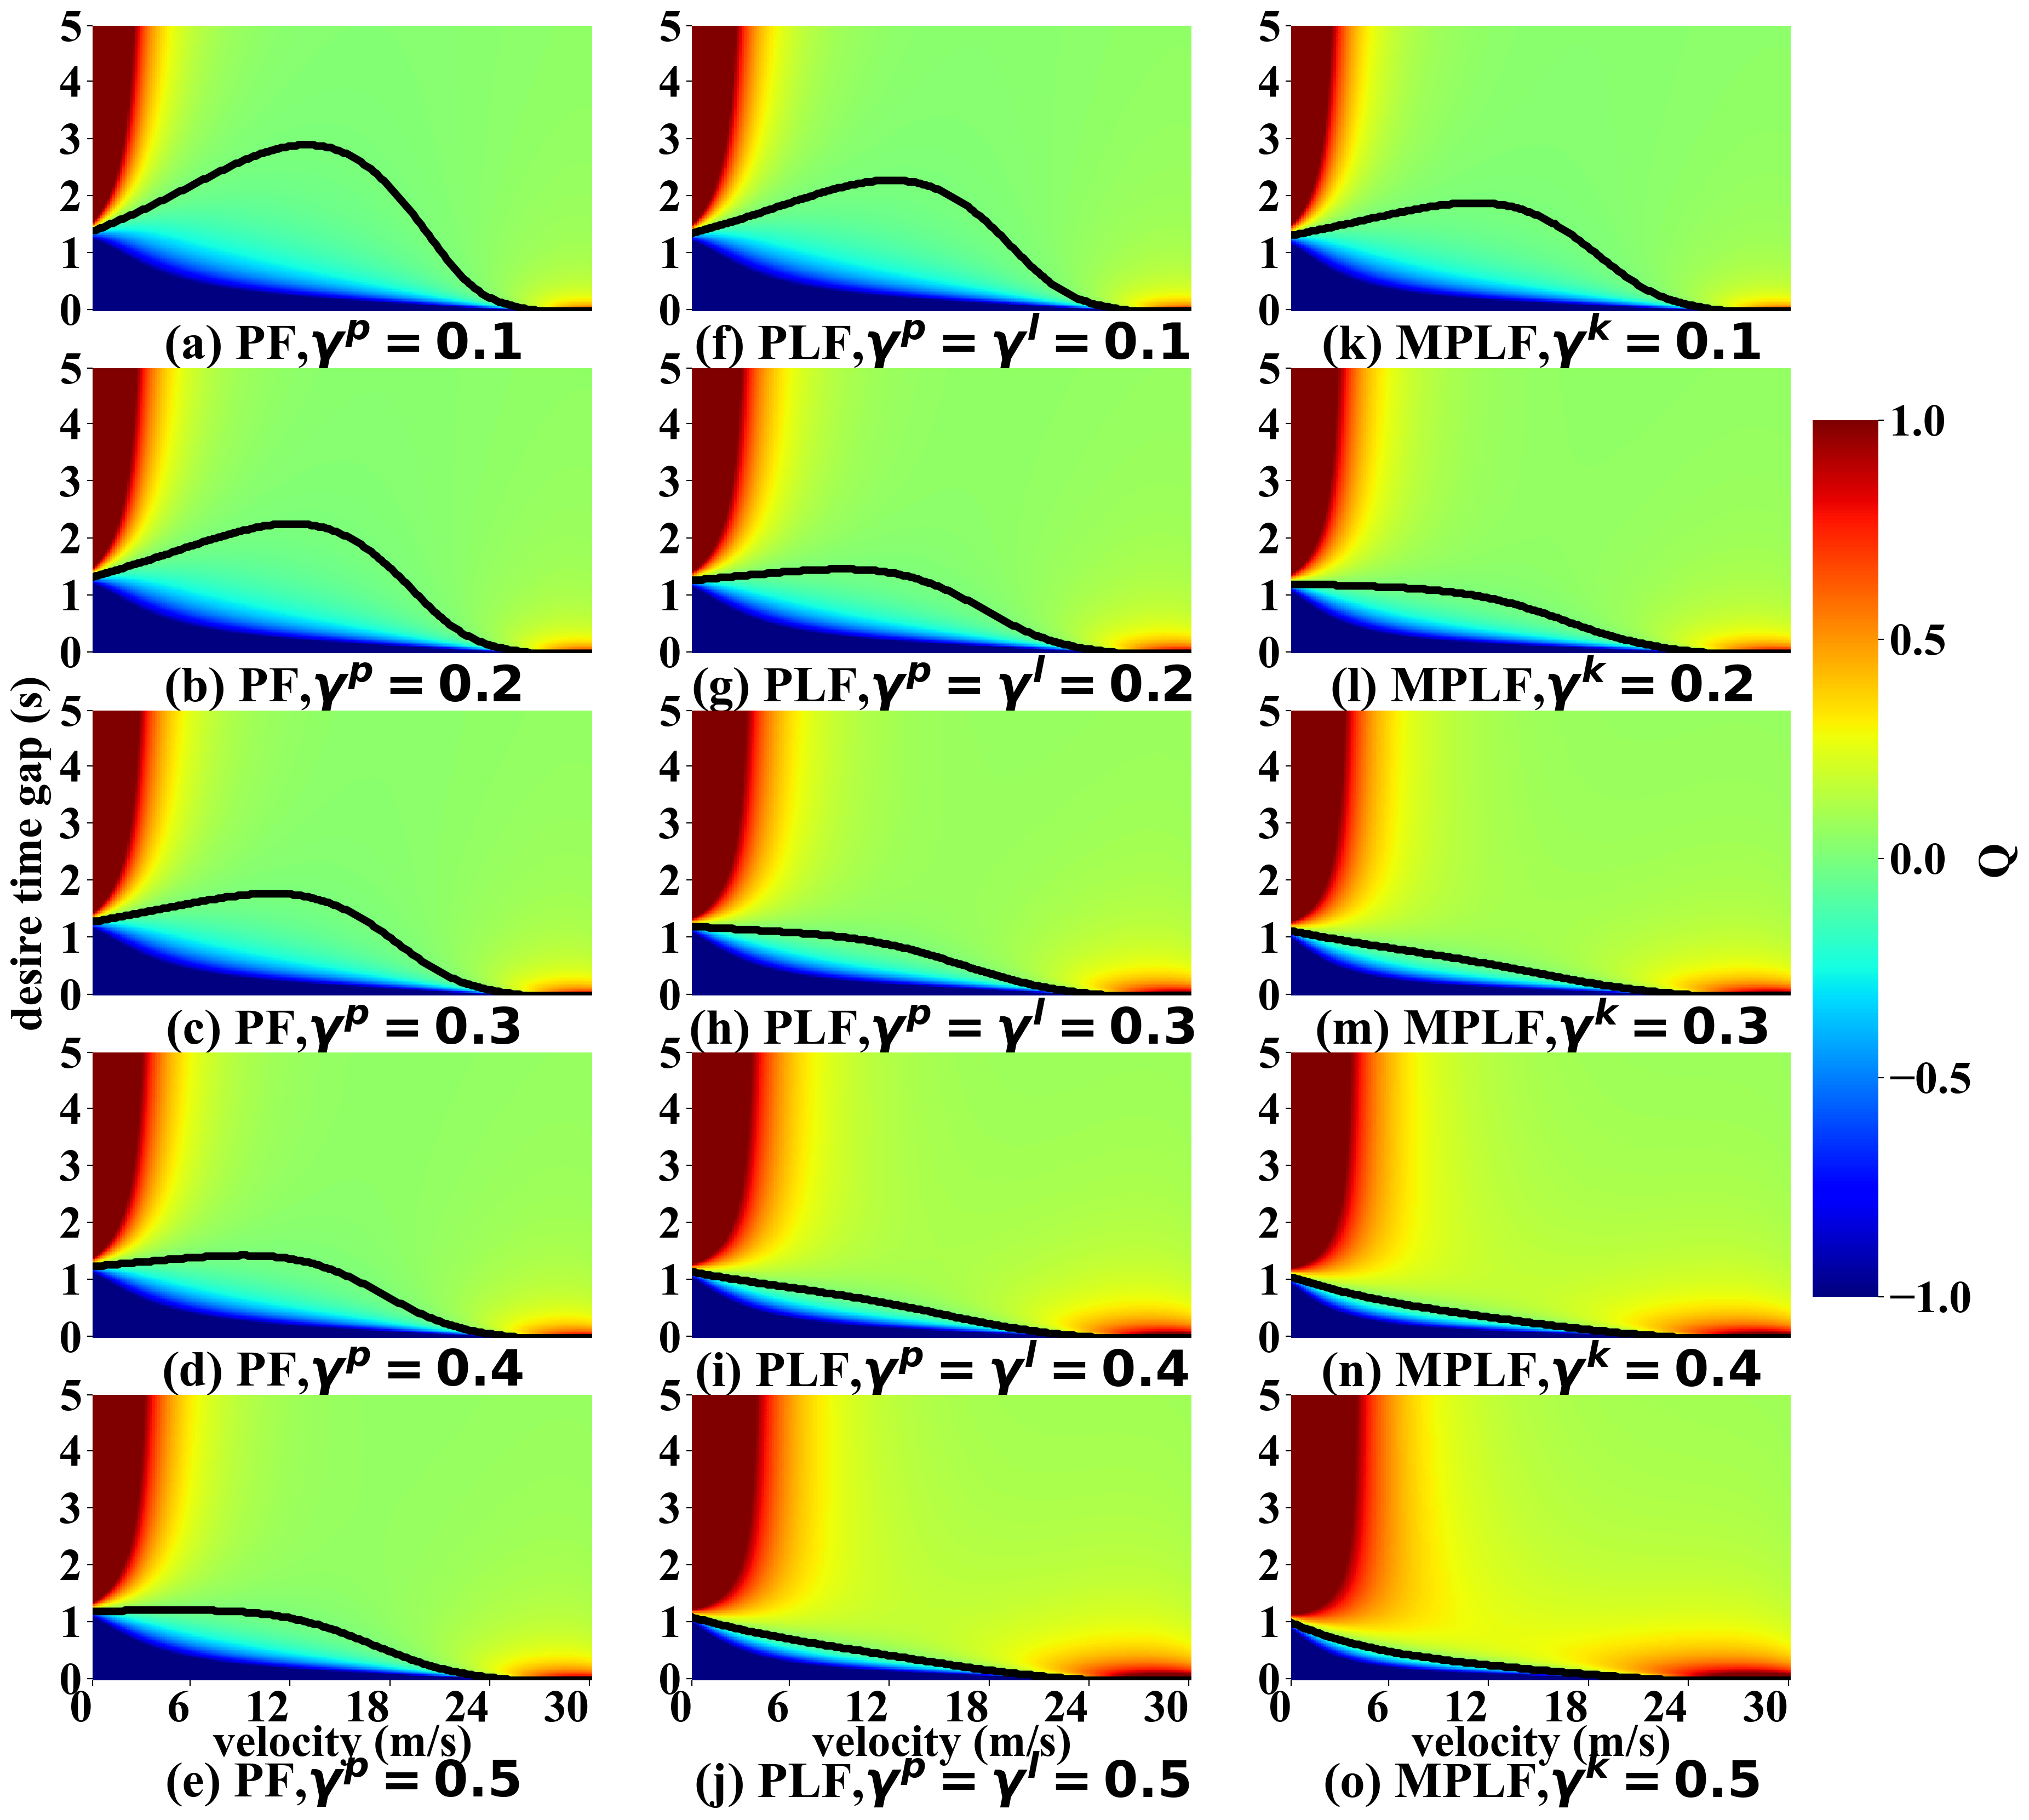
\includegraphics[width=9cm]{fig4.png}
  \caption{~The heatmaps in the velocity-desire time gap of different IFTs under different parameters setting. (a)-(e) the case of PF; (f)-(j) the case of PLF; (k)-(o) the case of MPLF.}
  \label{Figure4}
\end{figure}

% \textcolor[rgb]{1,0,0}{\textbf{resubmit the heatmaps of three IFTs under different parameters.}}

It can be clearly found in Fig.~\ref{Figure4}, margin stable curves of all IFTs decline as parameters setting increases, which means that an appropriate increase in weighting coefficient of communication gain can help reduce desire time gap without losing head-to-tail string stability. From another perspective, the curve of all IFTs with lower parameter settings will have a significant peak as the velocity increases. However, as for PF, this peak is not disappeared even if the parameter is set to 0.5, while the PLF and MPLF only need 0.3 to suppress. As for the differences between different parameters, the curves show a trend of getting closer with the parameters increasing. Moreover, the control of the vehicle will tend to follow the control strategy of the preceding vehicle rather than use its own, which means that the controller relies more on communication. However, the communication environment is not reliable enough to make decisions only based on the information communicated yet since the illegal channel occupation and obstacle interference are everywhere. For the reasons above, a more significant parameter value is not necessary to improve string stability, so we choose $\gamma_p=\gamma_l=\gamma_k=0.3$ in the following simulations.


\subsubsection{Simulation validation of theoretical results}
\label{Section 5.2.3}

% To verify the results of theoretical numerical analysis from the perspective of short-wave stability of traffic flow, two validation scheme was adopted as: 1.the stability region validation, 2.the specific response of the CACC platoon under disturbance under open boundary conditions. 

To verify the results of theoretical numerical analysis from the perspective of short-wave stability of traffic flow, the stability region validation is conducted in the disturbance \textit{Type \uppercase\expandafter{\romannumeral1}}.


\textit{stability region validation}: To validate the stability region of different IFTs obtained in Section~\ref{Section 5.2.1}, simulations under traffic settings with different values of desire time gap and velocity are conducted. Here we divided the velocity range ($0-30 m/s$) by an interval of $0.3 m/s$ where a break of 0.02s separated the desire time gap (0-2s). Note that the validation of the stability region is only conducted at 0-2s desire time gap since the margin curves of three IFTs are lower than 2s at the entire velocity range, and only disturbance \textit{Type \uppercase\expandafter{\romannumeral1}} is adopted to avoid too much computational burden. The stability region obtained by simulations is shown in Fig.~\ref{Figure5.2.3}, where the black curve shows the margin stable curve in the theoretical results, and the blue region depicts the stability region in simulation while the orange region depicts the instability region.

% \textcolor[rgb]{1,0,0}{\textbf{add stability region figure (desire time gap against speed) based on the simulation result, waiting results/new figure}}

\begin{figure}
  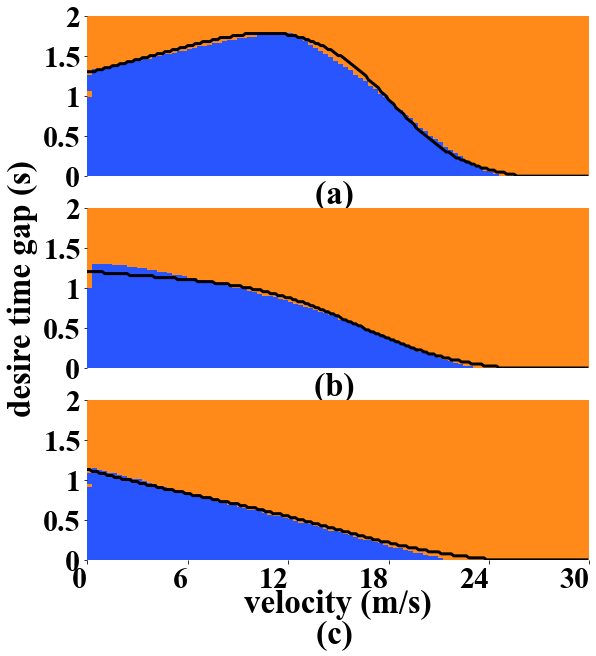
\includegraphics[width=9cm]{figextend1.png}
  \caption{~The heatmaps of simulation results in the velocity-desire time gap under different IFTs. (a) the case of PF; (b) the case of PLF; (c) the case of MPLF.}
  \label{Figure5.2.3}
\end{figure}

From Fig.~\ref{Figure5.2.3}, one conclusion that can be drawn is that the simulation results and theoretical results remain highly consistent since the margin stable curve almost coincides with the dividing line on the heatmaps. In addition, it is easier to ensure string stability that the desire time gap increases, both in theoretical and simulation results. It is important to note that when the velocity is in the interval close to 0 $m/s$, the desire time gap corresponding to the margin stable in the simulation result is lower than the margin stable curve. One reason for speculation is that the disturbance \textit{Type \uppercase\expandafter{\romannumeral1}} we applied is a pure acceleration disturbance causing its actual average velocity to deviate from 0 $m/s$ as the equilibrium velocity and is quite different from the equilibrium velocity. In general, the above results show that the theoretical results of linear stability analysis agree with those of the simulation of short-wave stability.


% \textit{specific response of the CACC platoon under disturbance}:


% \textcolor[rgb]{1,0,0}{\textbf{not Done}}

% Fig.~\ref{Figure5}-\ref{Figure6} show the time evolutions of the velocity and acceleration of the simulation platoon for the parameter $t_a=0.1,0.3,0.4,0.6s$.

% \textcolor[rgb]{1,0,0}{\textbf{Here all desire time gap can be added}}

% \begin{figure}
% 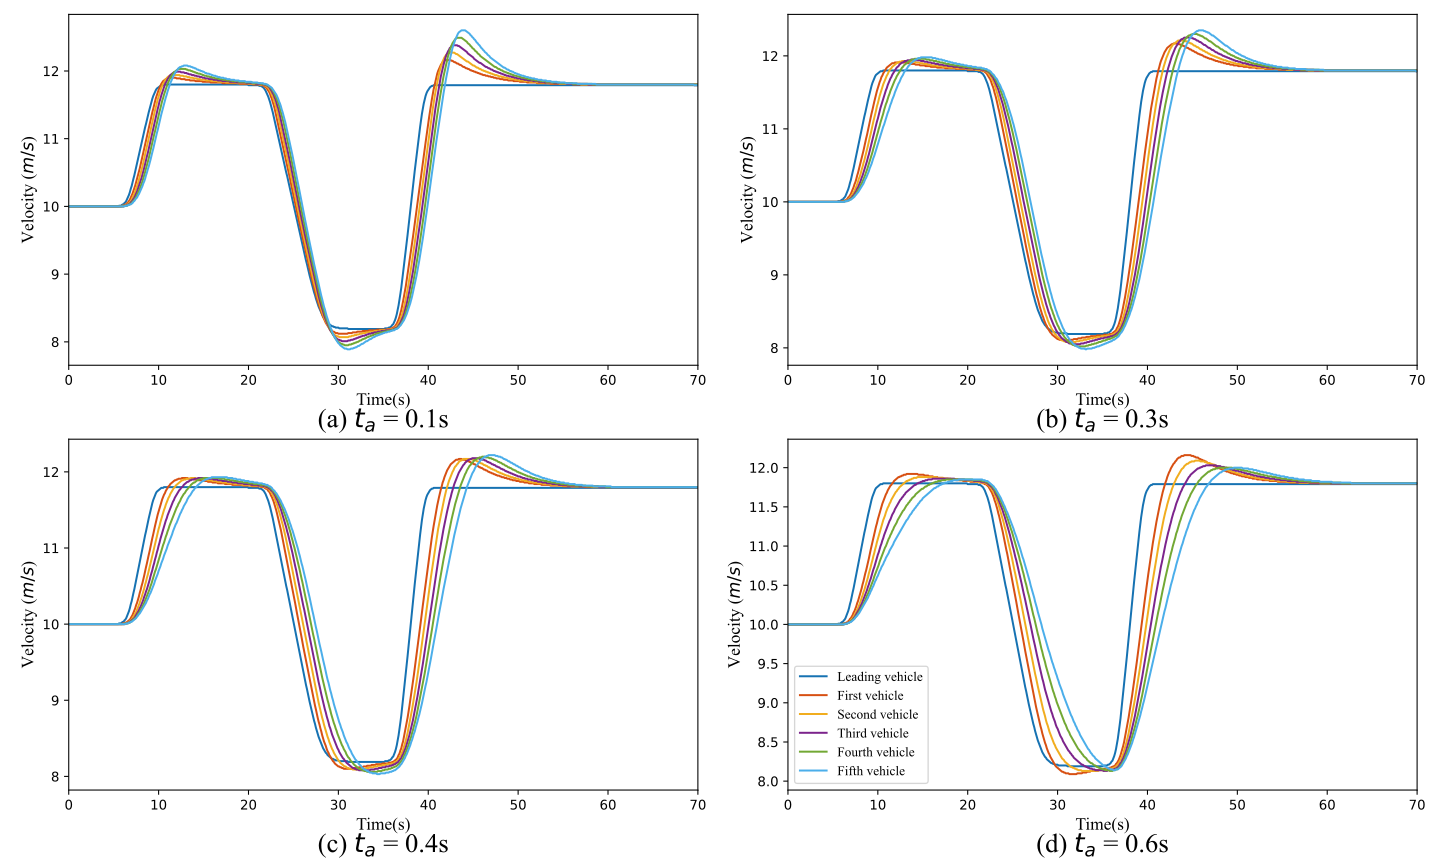
\includegraphics[width=9cm]{fig5.png}
% \caption{~Time evolutions of the velocity of the simulation platoon for the parameter $t_a=0.1,0.3,0.4,0.6s$.} 
% \label{Figure5}
% \end{figure}

% \begin{figure}
% 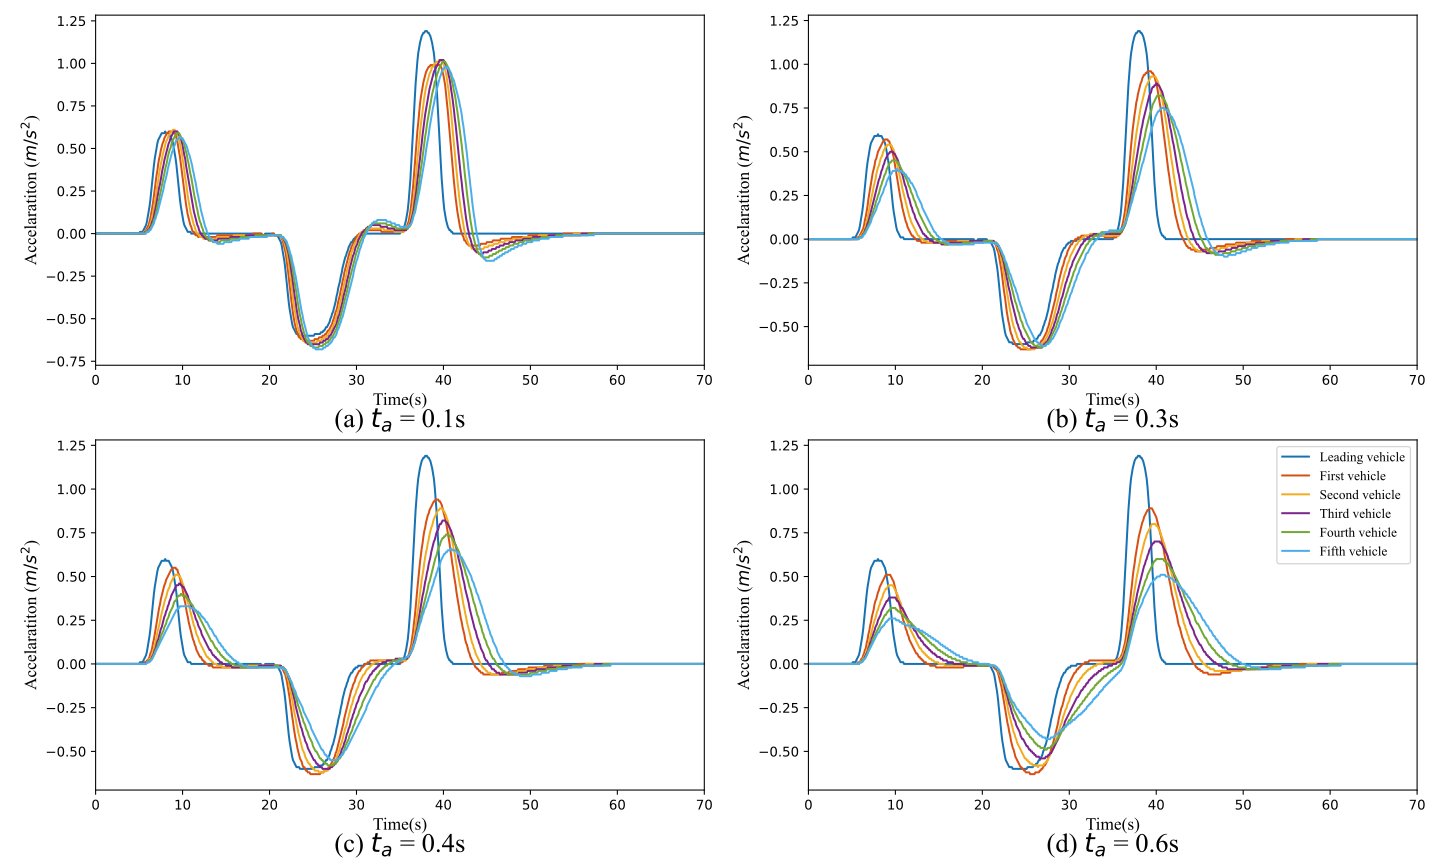
\includegraphics[width=9cm]{fig6.png}
% \caption{~Time evolutions of the acceleration of the simulation platoon for the parameter $t_a=0.1,0.3,0.4,0.6s$.} 
% \label{Figure6}
% \end{figure}

% From Fig.~\ref{Figure5}-\ref{Figure6}, we can clearly find that with the increase of the desire time gap $t_a$, the traffic oscillation generated by the sudden accelerating and decelerating of the leader vehicle MV gradually weakened in the CACC platoon. When $t_a=0.1,0.3,0.4s$, the disturbance increase propagates downstream with time as shown in Fig.~\ref{Figure5}-\ref{Figure6}, which indicates the CACC platoon is string instability, while the disturbance is gradually suppressed as it propagates downstream for $t_a=0.6s$. The above results show that the theoretical results of linear stability analysis agree with those of the simulation of short-wave stability.


\subsection{Comparison of robustness}
\label{Section 5.3}
In practical application, channel occupancy and the obstacle within the communication range make the communication environment not absolutely ideal, making it necessary to ensure the robustness of the corresponding IFTs. Notice that the unreliable communication environment mentioned here refers to interference on the effect of communication, and cyber-attacks are not considered since the corresponding network security strategy should be activated. There are many indicators that characterize unreliable communication environments, such as Channel Busy Ratio (CBR), delay, Packet Error Ratio (PER), and Inter-Transmit Time (ITT). As for CBR and ITT, the effect on communication is reflected in PER. According to the report on the fourteenth meeting of IMT-2020 (5G) Promotion Group Cellular-Vehicle-to-everything Working Group, delays remain stable and below 61.5ms with 110 On-Board Units (OBUs) within a 100m radius. Therefore, PER is selected as the indicator to represent the unreliable communication environment. To verify the robustness of different IFTs, we simulated the CACC platoon equipped with different IFTs in a non-ideal communication environment with several PER (5\%, 10\%, 20\%) and 10Hz communication frequencies. Here we divided the velocity range ($0-30 m/s$) by an interval of $0.75 m/s$ where a break of 0.05s separated desire time gap (0-2s). IFT parameter settings similar to those in Section~\ref{Section 5.1} are adopted in the simulation, with three types of disturbances applied. In addition, to quantify the effects of unreliable communication, we choose the PER of 0\% as the benchmark for comparison and the absolute value of the velocity difference as the indicator to represent the impact, which a higher value indicates a larger impact. The simulation results are shown in Fig.~\ref{fig_5.3.1}, Fig.~\ref{fig_5.3.2}, and Fig.~\ref{fig_5.3.3}.

\begin{figure}
  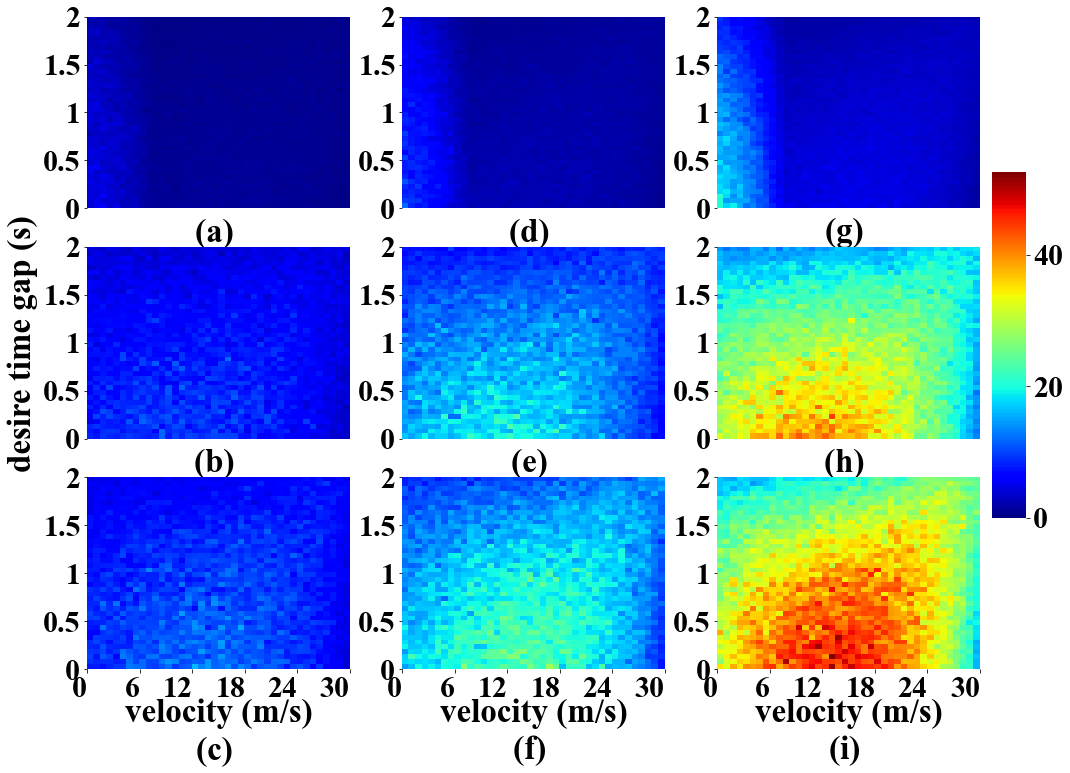
\includegraphics[width=9cm]{fig_5.3.1.png}
  \caption{~The heatmaps of the velocity difference against ideal communication among three IFTs with different PER under disturbance \textit{Type \uppercase\expandafter{\romannumeral1}}. (a)-(c) the case with 5\% PER; (d)-(f) the case with 10\% PER; (g)-(i) the case with 20\% PER. (a),(d),(g) The case of PF; (b),(e),(h) The case of PLF; (c),(f),(i) The case of MPLF.}
  \label{fig_5.3.1}
\end{figure}
\begin{figure}
  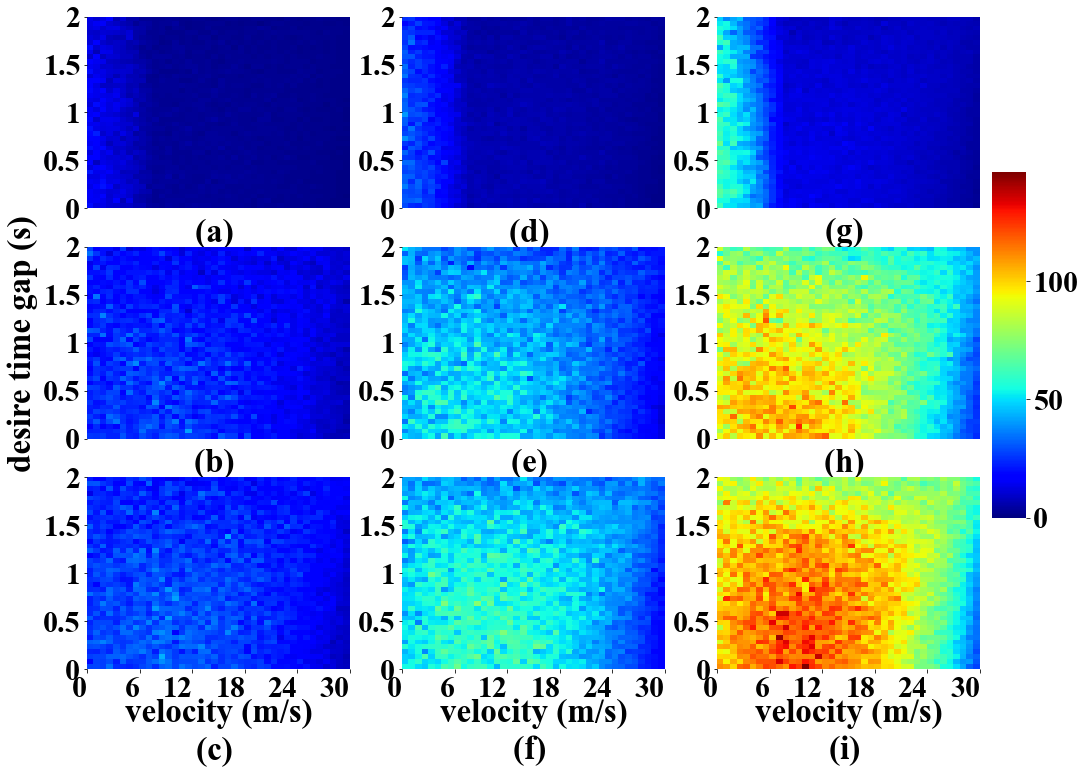
\includegraphics[width=9cm]{fig_5.3.2.png}
  \caption{~The heatmaps of the velocity difference against ideal communication among three IFTs with different PER under disturbance \textit{Type \uppercase\expandafter{\romannumeral2}}. (a)-(c) the case with 5\% PER; (d)-(f) the case with 10\% PER; (g)-(i) the case with 20\% PER. (a),(d),(g) The case of PF; (b),(e),(h) The case of PLF; (c),(f),(i) The case of MPLF.}
  \label{fig_5.3.2}
\end{figure}
\begin{figure}
  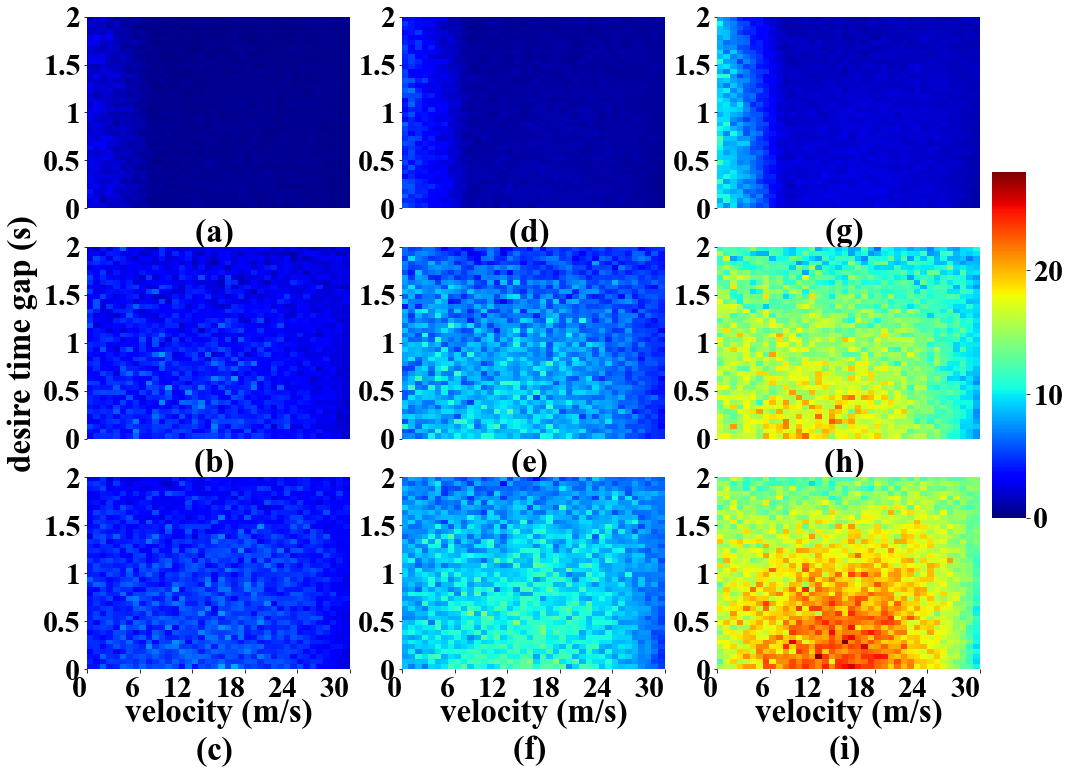
\includegraphics[width=9cm]{fig_5.3.3.png}
  \caption{~The heatmaps of the velocity difference against ideal communication among three IFTs with different PER under disturbance \textit{Type \uppercase\expandafter{\romannumeral3}}. (a)-(c) the case with 5\% PER; (d)-(f) the case with 10\% PER; (g)-(i) the case with 20\% PER. (a),(d),(g) The case of PF; (b),(e),(h) The case of PLF; (c),(f),(i) The case of MPLF.}
  \label{fig_5.3.3}
\end{figure}



First of all, the influence of equivalent PERs on different IFTs is analyzed. We can sum up from Fig.~\ref{fig_5.3.1} - \ref{fig_5.3.3} that PER has the minor impact on PF, while MPLF has the biggest. At a PER of 20\%, PFs can maintain the same state as the one with ideal communication in most of the control space. On the contrary, PLF and MPLF have noteworthy differences. This phenomenon is quite understandable because more communication demand leads to more communication failures under the same PERs, which further seriously impacts car-following behaviors. As for the influence of different PERs, a reasonable conclusion can be drawn that its impact greatly increases with the rise of PER. Considering the impact of different disturbance types, we can find that \textit{Type \uppercase\expandafter{\romannumeral2}} has far more impact than \textit{Type \uppercase\expandafter{\romannumeral1}} and \textit{Type \uppercase\expandafter{\romannumeral3}}. The phenomenon can be interpreted that \textit{Type \uppercase\expandafter{\romannumeral2}} has the greatest scale of duration and magnitude than the other two, which brings the most significant advantage with ideal communication. However, this advantage will be weakened when the communication is unreliable. Moreover, the larger the weakening, the bigger the influence.

As for the specific impact of PER, we have selected the case with velocity at $10 m/s$, PER at 20\%, and desire time gap at $1.2 s$ as an example for analysis, the curves of velocities and accelerations are shown in Fig.~\ref{Figure7}.


\begin{figure*}
  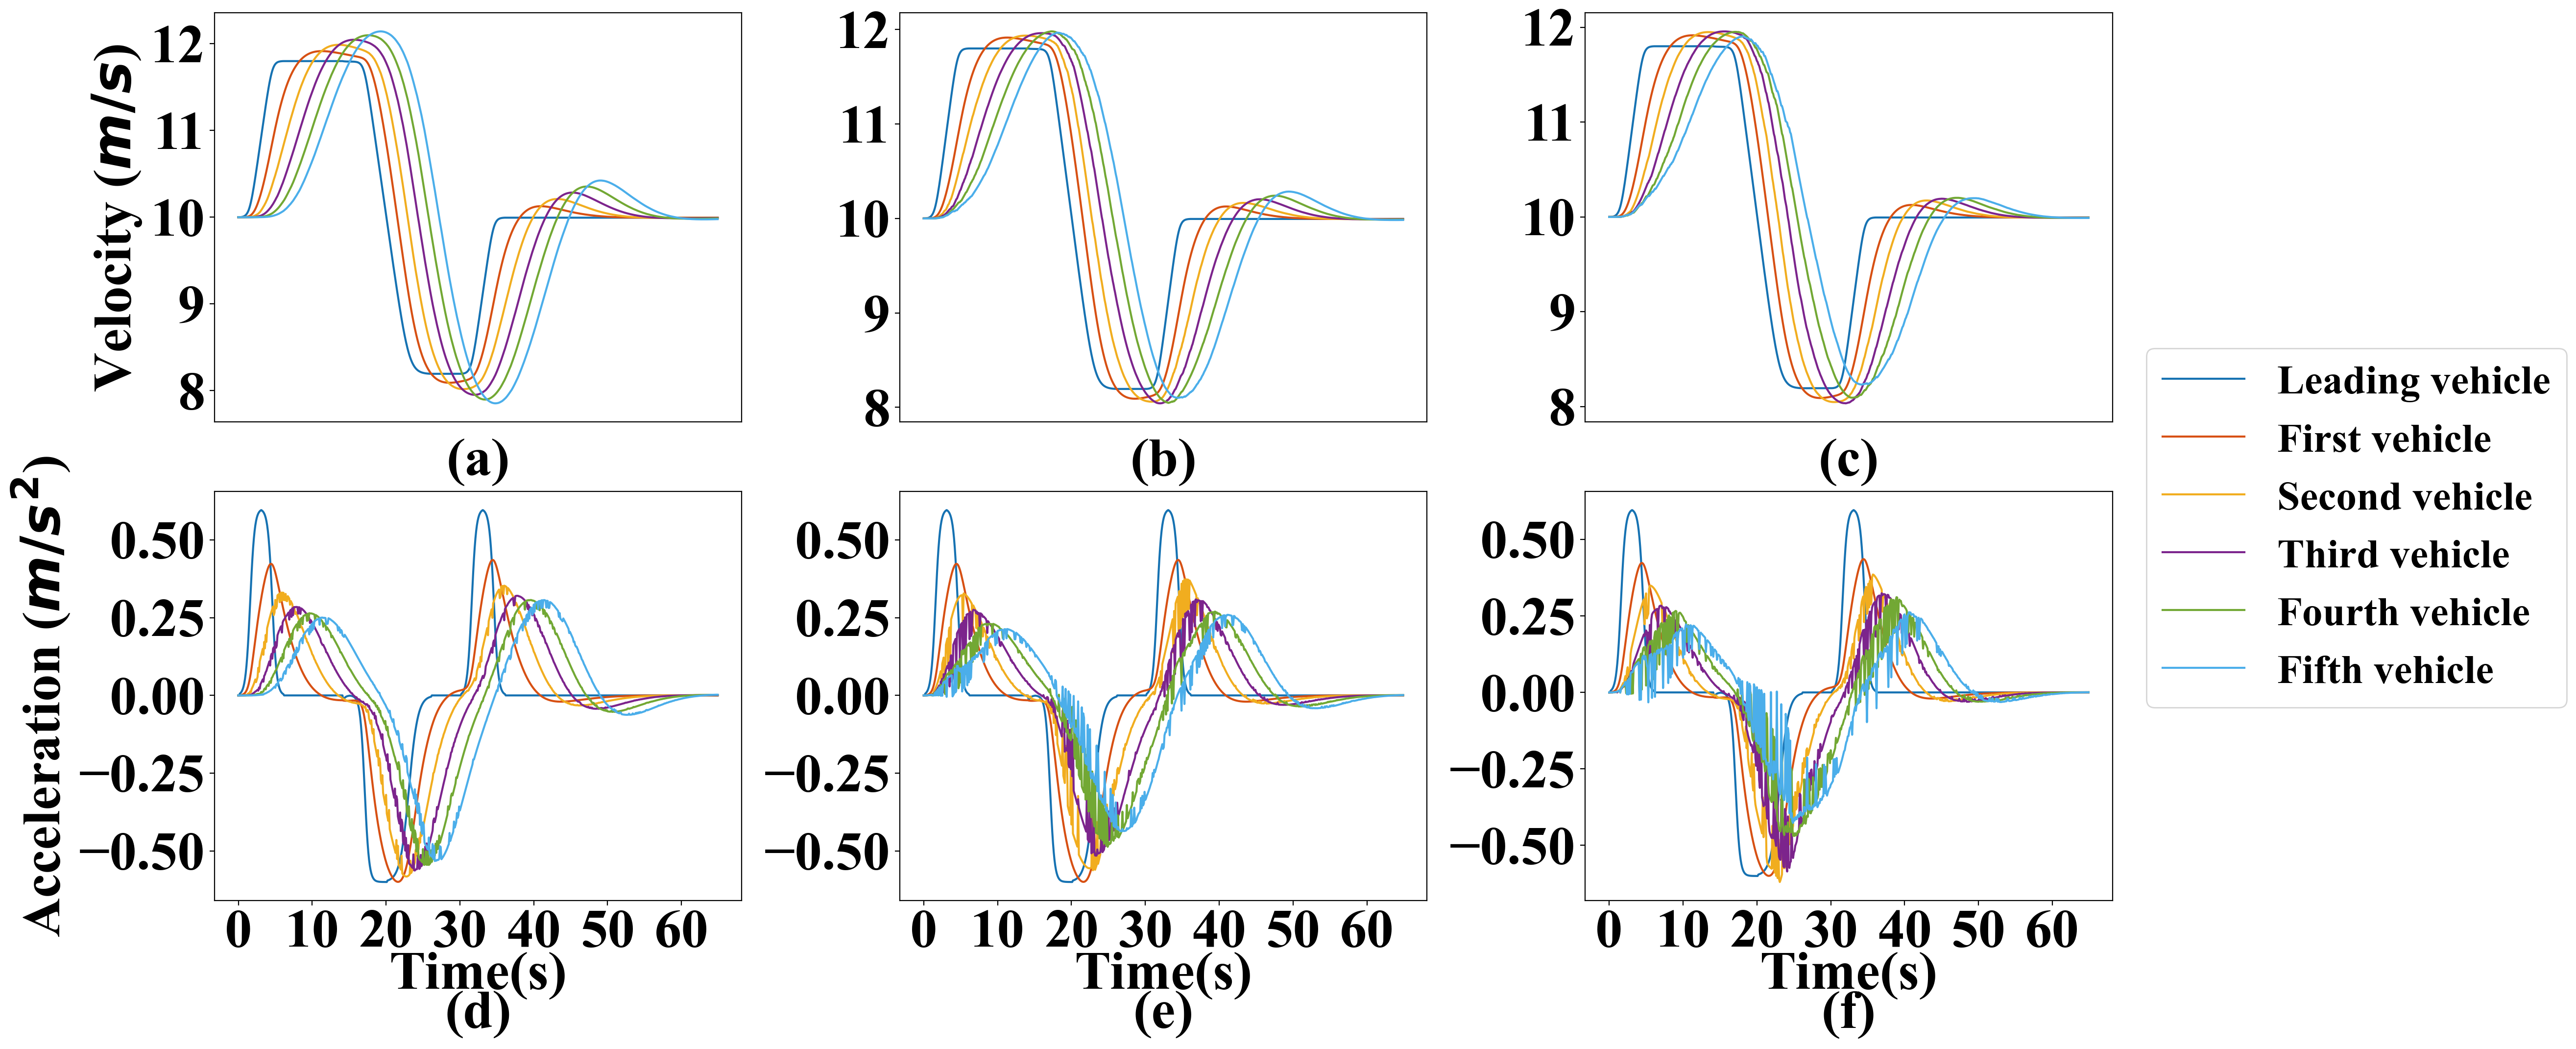
\includegraphics[width=18cm]{fig_5.3.4.png}
  \caption{~Time evolutions of the velocity and acceleration of simulation platoon for different IFTs with the velocity at $10 m/s$, PER at 20\%, and desire time gap at $1.2 s$. (a)-(c) the subplots of the velocity curves; (d)-(f) the subplots of the velocity curves; (a),(d) the case of PF; (b),(e) the case of PLF; (c),(f) the case of MPLF.}
  \label{Figure7}
\end{figure*}

PER appears as a sudden increase or decrease of the acceleration in Fig.~\ref{Figure7}. Admittedly, poor communication quality can significantly affect the stability of the CACC platoon, especially in continuous packet error. However, due to high communication frequency, the velocity curves of PF and PLF remain steady. At the same time, few disturbances on accelerations show that platoon controllers designed based on PF and PLF are robust against such communication failures. They can still guarantee smooth driving even under poor communication quality. On the other hand, platoon controllers designed based on MPLF are not robust against such communication failures and cannot maintain an appropriate time gap due to their dependence on ideal communication. Moreover, more communication requirements are needed for MPLF to achieve a smaller desire time gap, but the reduction in the desire time gap will bring a surge in communication requirements that is difficult to achieve. According to corresponding research \citep{hafeez2013performance}, the failure rate of communication is $16\%$ when the communication frequency is 2 packet/s, and when the communication frequency is 5 packet/s, the failure rate is $38\%$. This indicates that as the communication demand in the same channel approaches the channel bandwidth, the communication failures will significantly increase. Therefore, the gain on the margin stable curve and its negative impact on communication instability should be considered balanced.
To summarize, PF and PLF are more suitable IFTs in terms of robustness.

\subsection{Comparison of traffic safety}
\label{Section 5.4}

In addition to stability, safety is another essential reference factor for controller design. Two indicators, such as Maximum Time To Collision (MTTC) and Deceleration Rate to Avoid the Crash (DRAC), are selected to compare the security performance of platoon controllers based on different IFTs. The corresponding indicators are calculated as follows:
\begin{equation}
  MTTC_{t}=\frac{v_{F, t}-v_{L, t} \pm \sqrt{\left(v_{F, t}-v_{L, t}\right)^{2}+2 \Delta a_{t}\left(x_{L, t}-x_{F, t}-D_{L}\right)}}{\Delta a_{t}},
\end{equation}
\begin{equation}
  DRAC_{F, t}=\frac{\left(v_{F, t}-v_{L, t}\right)^{2}}{2\left(x_{L, t}-x_{F, t}-D_{L}\right)},
\end{equation}
where $x_{L,t}$ and $x_{F,t}$ denotes the positions of the leading vehicle and the following vehicle at time t, respectively; $v_{F,t}$ and $v_{L,t}$ are their velocities at time t; $D_L$ is the length of the leading vehicle; $\Delta a_t$ is the relative acceleration of conflicting vehicles at time t; $t_{F,t}$ and $t_{L,t}$ are the time of following vehicle arrives and leading vehicle leaves encroachment time. Simulation is implemented based on similar IFT parameter settings in Section~\ref{Section 5.1}, and all disturbance types are adopted in simulation. Fig.~\ref{Figure3_1} and Fig.~\ref{Figure3_2} show the heatmap of different IFTs compared with pure MV environment as the baseline on various indicators under three disturbances in the control space (velocity-desire time gap). It should be noted that the MTTC is the larger, the safer, while the DRAC is the smaller, the safer. Therefore, the improvement rate mentioned here refers to the increased proportion of IFT compared to MV for MTTC, representing the reduced proportion for DRAC. Moreover, the black curve in each subfigure represents the margin stable curve of the corresponding IFT.

% \begin{table}\large
%     \centering
%     \setlength{\abovecaptionskip}{0pt}
%     \setlength{\belowcaptionskip}{10pt}%设置标题与表格的距离
%     \caption{~Definitions and formulas of indicators used to evaluate safety.}
%     \resizebox{0.5\textwidth}{!}{
%     \renewcommand\arraystretch{1.5}
%         \begin{tabular}{|c|c|c|}
%         \hline  & Definition & Calculation formulas \\
%         \hline \multirow{2}{*}{MTTC} & \multirow{2}{*}{Maximum Time To Collision} & 
%         \multicolumn{1}{|l|}{$MTTC_{t}=$}\\
%         &&\multicolumn{1}{|c|}{$\frac{v_{F, t}-v_{L, t} \pm \sqrt{\left(v_{F, t}-v_{L, t}\right)^{2}+2 \Delta a_{t}\left(x_{L, t}-x_{F, t}-D_{L}\right)}}{\Delta a_{t}}$}\\
%         \hline DRAC & Deceleration Rate to Avoid the Crash & 
%         \multicolumn{1}{|l|}{$DRAC_{F, t}=\frac{\left(v_{F, t}-v_{L, t}\right)^{2}}{2\left(x_{L, t}-x_{F, t}-D_{L}\right)}$}\\
%         \hline
%         \end{tabular}
%     }
% \label{Table2}
% \end{table}

% \begin{table}\large
%   \centering
%   \setlength{\abovecaptionskip}{0pt}
%   \setlength{\belowcaptionskip}{10pt}%设置标题与表格的距离
%   \caption{~Definitions and formulas of indicators used to evaluate safety.}
%   \resizebox{0.5\textwidth}{!}{
%   \renewcommand\arraystretch{1.5}
%       \begin{tabular}{|c|c|c|}
%       \hline  & Definition & Calculation formulas \\
%       \hline TTC  & Time To Collision &  $T T C_{t}=\frac{x_{L, t}-x_{F, t}-D_{L}}{v_{F, t}-v_{L, t}} ; \forall\left(v_{F, t}-v_{L, t}\right)>0$\\
%       \hline \multirow{2}{*}{MTTC} & \multirow{2}{*}{Maximum Time To Collision} & 
%       \multicolumn{1}{|l|}{$MTTC_{t}=$}\\
%       &&\multicolumn{1}{|c|}{$\frac{v_{F, t}-v_{L, t} \pm \sqrt{\left(v_{F, t}-v_{L, t}\right)^{2}+2 \Delta a_{t}\left(x_{L, t}-x_{F, t}-D_{L}\right)}}{\Delta a_{t}}$}\\
%       \hline DRAC & Deceleration Rate to Avoid the Crash & 
%       \multicolumn{1}{|l|}{$DRAC_{F, t}=\frac{\left(v_{F, t}-v_{L, t}\right)^{2}}{2\left(x_{L, t}-x_{F, t}-D_{L}\right)}$}\\
%       \hline
%       \end{tabular}
%   }
% \label{Table2}
% \end{table}

\begin{figure}
  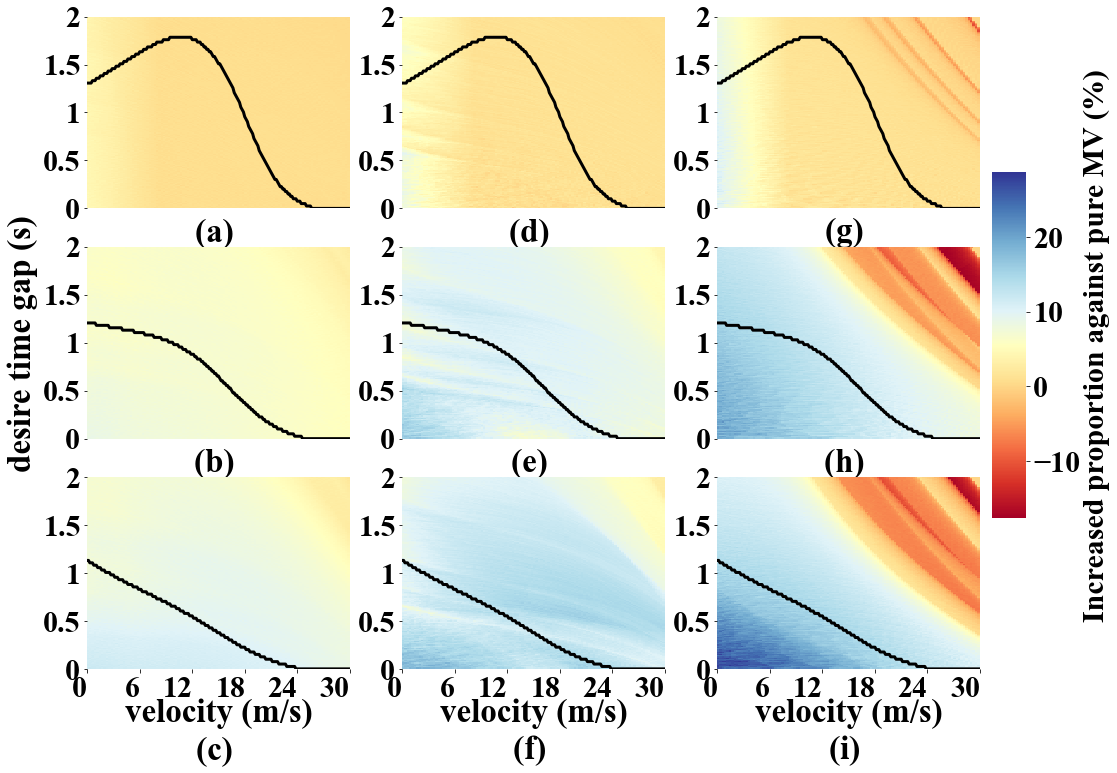
\includegraphics[width=9cm]{fig5.3_1.png}
  \caption{~Increased proportion heatmaps of MTTC among three IFTs against pure MV under three disturbances. (a)-(c) the case under disturbance \textit{Type \uppercase\expandafter{\romannumeral1}}; (d)-(f) the case under disturbance \textit{Type \uppercase\expandafter{\romannumeral2}}; (g)-(i) the case under disturbance \textit{Type \uppercase\expandafter{\romannumeral3}}. (a),(d),(g) The case of PF; (b),(e),(h) The case of PLF; (c),(f),(i) The case of MPLF.}
  \label{Figure3_1}
\end{figure}

\begin{figure}
  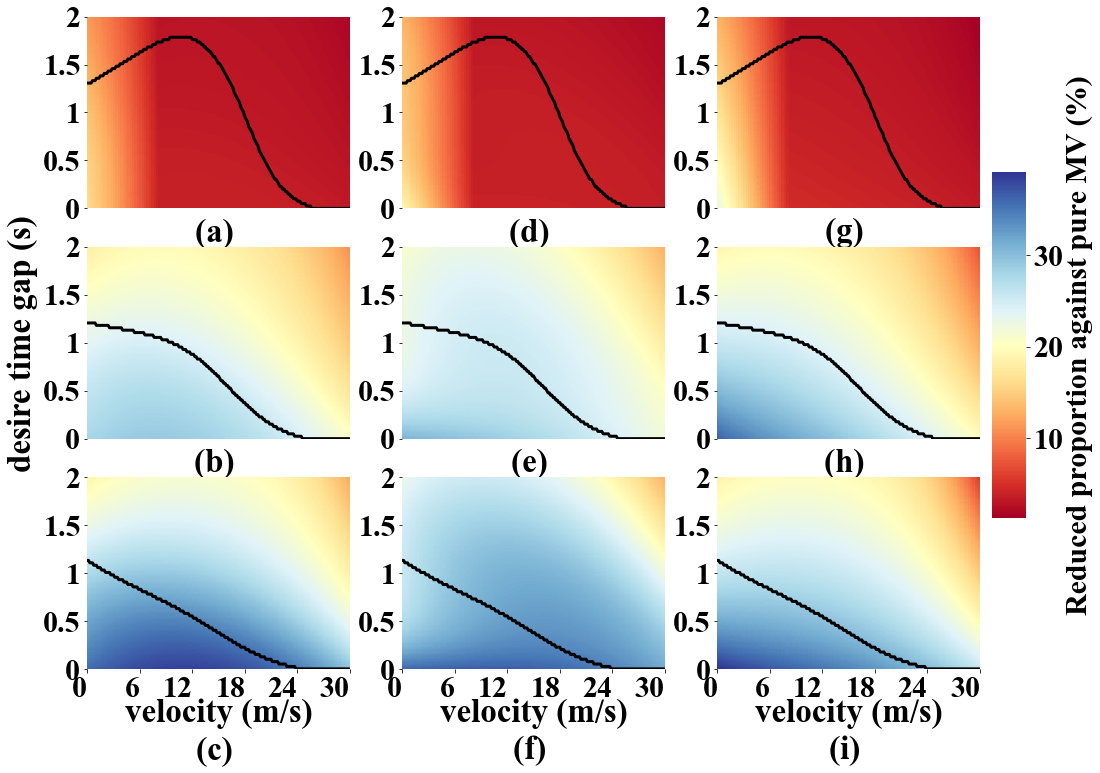
\includegraphics[width=9cm]{fig5.3_2.png}
  \caption{~Reduced proportion heatmaps of DRAC among three IFTs against pure MV under three disturbances. (a)-(c) the case under disturbance \textit{Type \uppercase\expandafter{\romannumeral1}}; (d)-(f) the case under disturbance \textit{Type \uppercase\expandafter{\romannumeral2}}; (g)-(i) the case under disturbance \textit{Type \uppercase\expandafter{\romannumeral3}}. (a),(d),(g) The case of PF; (b),(e),(h) The case of PLF; (c),(f),(i) The case of MPLF.}
  \label{Figure3_2}
\end{figure}

First, we focus on the distribution of heatmaps in each subplot. No matter what kind of disturbances and what kind of IFTs, heatmaps all show a trend that the increased proportion decreases as the velocity and desire time gap increase in the control space (velocity-desire time gap). Notices that for DRAC, all IFTs are able to maintain better safety conditions against MVs, while some areas are not as good as MVs for MTTC, which may be due to significantly increased string stability of MVs at the high desire time gap and velocity.

The second thing to note is the difference in heatmaps between different IFTs under the same disturbance. From Fig.~\ref{Figure3_1} and \ref{Figure3_2}, a phenomenon can find that IFTs with more communication information can maintain better safety conditions that are significantly larger than the case of PF when velocity and desire time gap is low. However, from the point of view of the whole control space, IFTs with more communication information are greatly affected by the change of velocity and desire time gap, while PF has little difference.

As for the differences between different disturbances in the same IFT, most groups of subplots in Fig.~\ref{Figure3_1} and Fig.~\ref{Figure3_2} show that the degree of impact on MTTC gradually increases from \textit{Type \uppercase\expandafter{\romannumeral1}} to \textit{Type \uppercase\expandafter{\romannumeral3}}. This phenomenon is easy to understand because the three disturbances change more and more dramatically on the acceleration, which is not conducive to traffic safety. However, the law above does not apply to DRAC for MPLF. Better safety conditions can be provided under disturbance \textit{Type \uppercase\expandafter{\romannumeral1}} than under the \textit{Type \uppercase\expandafter{\romannumeral2}} or \textit{Type \uppercase\expandafter{\romannumeral3}} disturbance for MPLF.

Given the above, using PLF and MPLF can improve traffic safety compared to MV and PF in most scenarios. In addition, having more communication information helps maintain better security conditions at low velocity but worsens at high velocity. PLF and MPLF are therefore more inclined to adopt than PF from the point of view of traffic safety.
% It can be found from Fig.~\ref{Figure8} that the application of CACC can significantly improve safety compared to purely manual driving no matter what IFT is used. However, the impact of different IFTs on safety indicators is distinct. For example, adopting PLF or MPLF can cause nearly twice the optimization effect compared to PF, while the difference between PLF and MPLF is tiny. When we pay attention to the difference between PLF and MPLF, we can find that PLF can still maintain a certain advantage compared to MPLF which may be due to the excessive dependence of MPLF on the information from the preceding vehicle. In general, PLF is the best among the three IFTs from the perspective of safety.


% A simulation experiment is also carried out with different velocities and desire time gaps to explore the change of the safety indicators in the region of velocity-desire time gap (for simplicity, here, only the DRAC is selected as the comparison indicator). Based on the safety indicator DRAC, optimization heatmaps of three IFTs relative to MV are shown in Fig.~\ref{Figure9} where value is expressed as a percentage.

% \begin{figure}
% 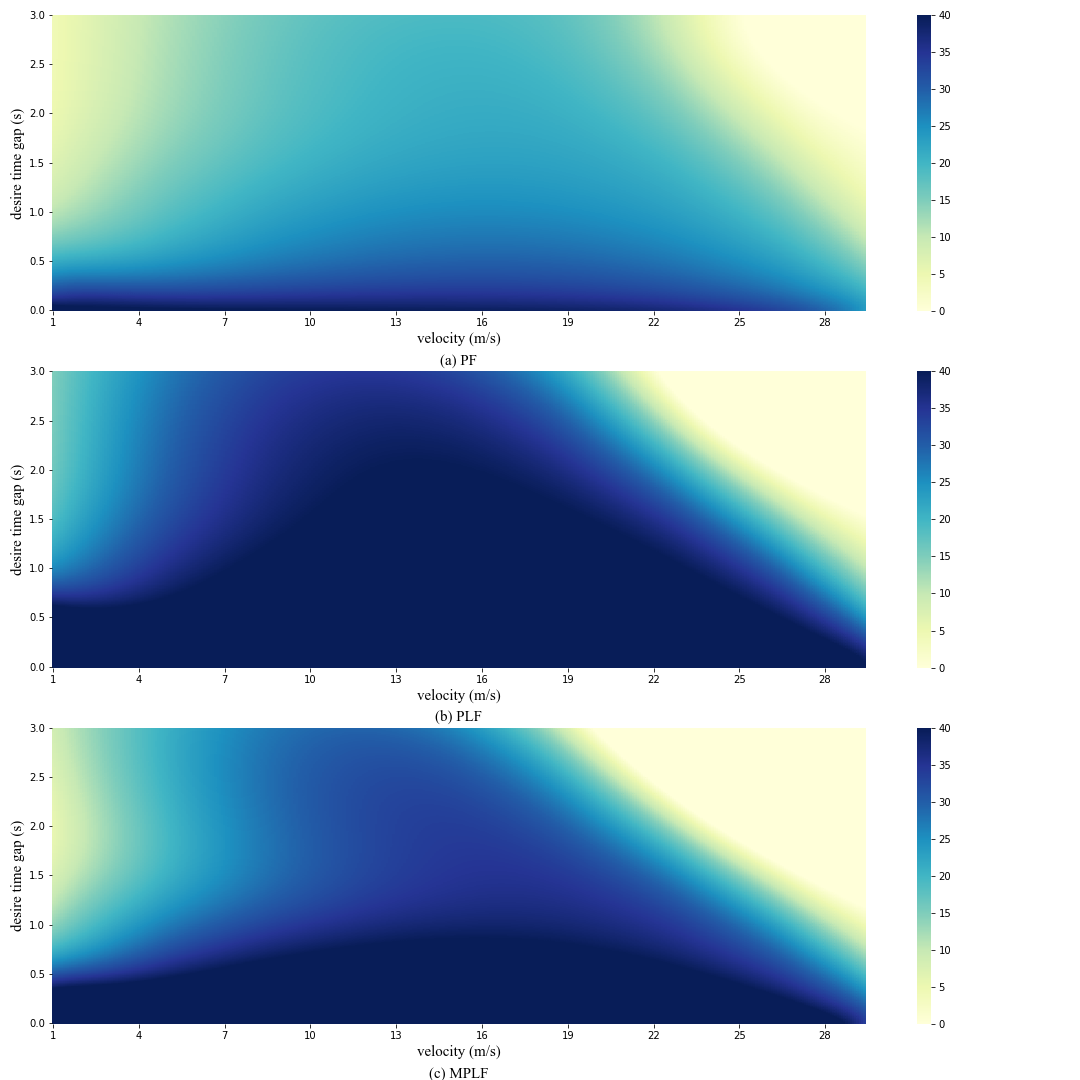
\includegraphics[width=9cm]{fig9.png}
% \caption{~Improvement rate heatmap of DRAC among three IFTs against pure MV.} 
% \label{Figure9}
% \end{figure}

% The improvement rate heatmaps of the three IFTs all show a trend that the improvement rate first increases and then decreases as the velocity increases. If PLF is adopted, the improvement rate can reach 40\% and above regardless of desired time gap. From the perspective of the desire time gap, it is found that the improvement rate decreases with the increase of the desire time gap. The phenomenon may be explained by that pure MV vehicles tend to be more and more stable with the improvement of the desire time gap. At the same time, CACCs remain stable so that the relative improvement rate is getting smaller and smaller. In addition, when we focus on the differences between the three IFTs, we find that adopting PLF or MPLF can maintain a significant gain compared to PF, and PLF is better than MPLF, which is similar to the conclusion in Fig.~\ref{Figure8}.

\subsection{Comparison of Eco-driving}
\label{Section 5.5}
With the substantial increase in the number of vehicles, CACCs are also considered a solution, so it is necessary to incorporate pollutant emissions into comparing different IFTs. Panis et al. \citep{panis2006modelling} established an emission model using a non-linear multivariate regression based on field measurement. The expression for calculation instantaneous traffic emission of a specific vehicle is:
\begin{small}
  \begin{equation}
    E_{i}(t)=\max \left[0, f_{1}\!+\!f_{2} v_{i}(t)\!+\!f_{3} v_{i}(t)^{2}\!+\!f_{4} a_{i}(t)\!+\!f_{5} a_{i}(t)^{2}\!+\!f_{6} v_{i}(t) a_{i}(t)\right],
  \end{equation}
\end{small}
where $E_i (t)$ is the pollutant emission for the vehicle in unit time (g/s); $f_1$ to $f_6$ are emission parameters for each type of pollutant; $v_i (t)$ is the velocity of the subject vehicle; and $a_i (t)$ is the acceleration of the subject vehicle. Values of emission parameters are provided in Table.\ref{Table3}. The simulation scenario is the same as Section~\ref{Section 5.1} with all three disturbances. The heatmaps of different IFTs under three disturbance types with pure MV setting as the baseline on three pollutant emissions are shown in Fig.~\ref{fig5.4_1}, Fig.~\ref{fig5.4_2}, and Fig.~\ref{fig5.4_3} with a black curve in each subplot representing the margin stable curve of the corresponding IFT.

\begin{table}
  \centering
  \setlength{\abovecaptionskip}{0pt}
  \setlength{\belowcaptionskip}{10pt}%设置标题与表格的距离
  \caption{~Parameters for Emission Model of Petrol Car.}
  \resizebox{0.5\textwidth}{!}{

    {\begin{tabular}{cccccccc} \toprule
          \multicolumn{2}{c}{Pollutant} & $f_{1}$                                 & $f_{2}$  & $f_{3}$   & $f_{4}$   & $f_{5}$   & $f_{6}$             \\ \midrule
          \multicolumn{2}{c}{$CO_{2}$}  & 5.53e-01                                & 1.61e-01 & -2.89e-03 & 2.66e-01  & 5.11e-01  & 1.83e-01            \\ \midrule
          \multirow{2}*{$NO_{x}$}       & $a \geq-0.5 \mathrm{~m}/\mathrm{s}^{2}$ & 6.19e-04 & 8.00e-05  & -4.03e-06 & -4.13e-04 & 3.80e-04 & 1.77e-04 \\ \cmidrule{2-8} & $a<-0.5 \mathrm{~m}/\mathrm{s}^{2}$ & 2.17 e-04 & 0 & 0 & 0 & 0 & 0 \\ \midrule
          \multirow{2}*{$VOC$}          & $a \geq-0.5 \mathrm{~m}/\mathrm{s}^{2}$ & 4.47e-03 & 7.32e-07  & -2.87e-08 & -3.41e-06 & 4.94e-06 & 1.66e-06 \\ \cmidrule{2-8} & $a<-0.5 \mathrm{~m}/\mathrm{s}^{2}$ & 2.63e-03 & 0 & 0 & 0 & 0 & 0 \\  \bottomrule
        \end{tabular}}
  }
  \label{Table3}
\end{table}

\begin{figure}
  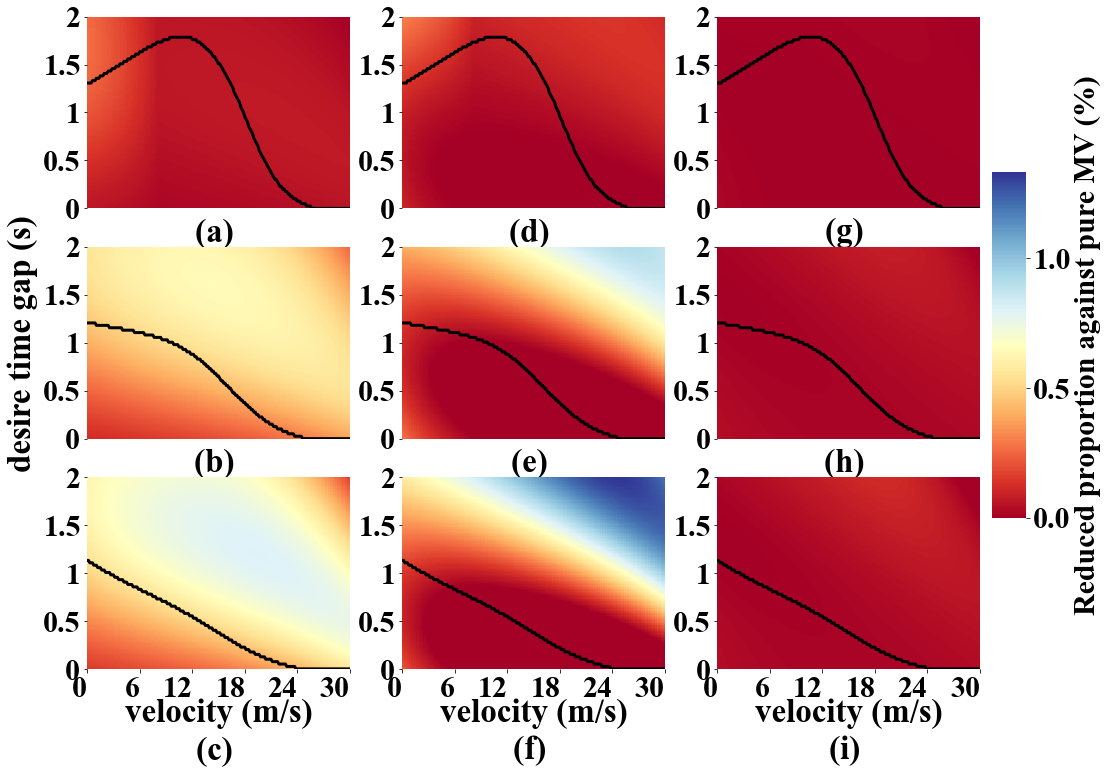
\includegraphics[width=9cm]{fig5.4_1.png}
  \caption{~Reduced proportion heatmaps of $CO_2$ among three IFTs against pure MV under three disturbances. (a)-(c) the case under disturbance \textit{Type \uppercase\expandafter{\romannumeral1}}; (d)-(f) the case under disturbance \textit{Type \uppercase\expandafter{\romannumeral2}}; (g)-(i) the case under disturbance \textit{Type \uppercase\expandafter{\romannumeral3}}. (a),(d),(g) The case of PF; (b),(e),(h) The case of PLF; (c),(f),(i) The case of MPLF.}
  \label{fig5.4_1}
\end{figure}

\begin{figure}
  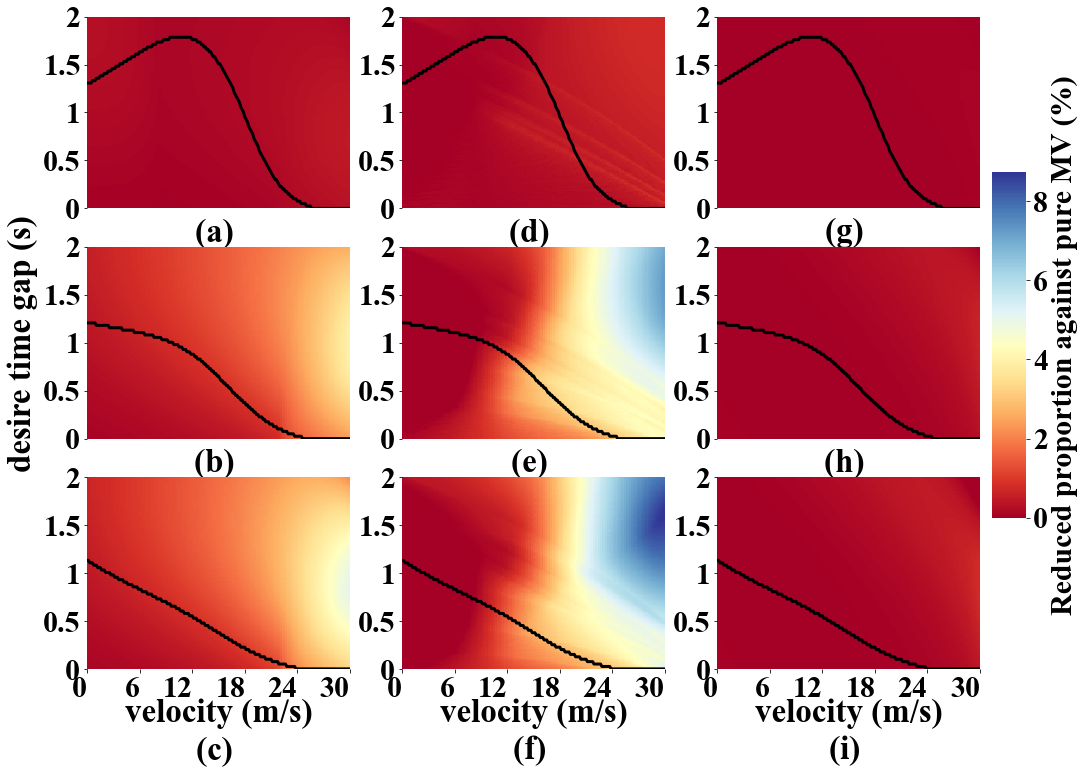
\includegraphics[width=9cm]{fig5.4_2.png}
  \caption{~Reduced proportion heatmaps of $NO_x$ among three IFTs against pure MV under three disturbances. (a)-(c) the case under disturbance \textit{Type \uppercase\expandafter{\romannumeral1}}; (d)-(f) the case under disturbance \textit{Type \uppercase\expandafter{\romannumeral2}}; (g)-(i) the case under disturbance \textit{Type \uppercase\expandafter{\romannumeral3}}. (a),(d),(g) The case of PF; (b),(e),(h) The case of PLF; (c),(f),(i) The case of MPLF.}
  \label{fig5.4_2}
\end{figure}

\begin{figure}
  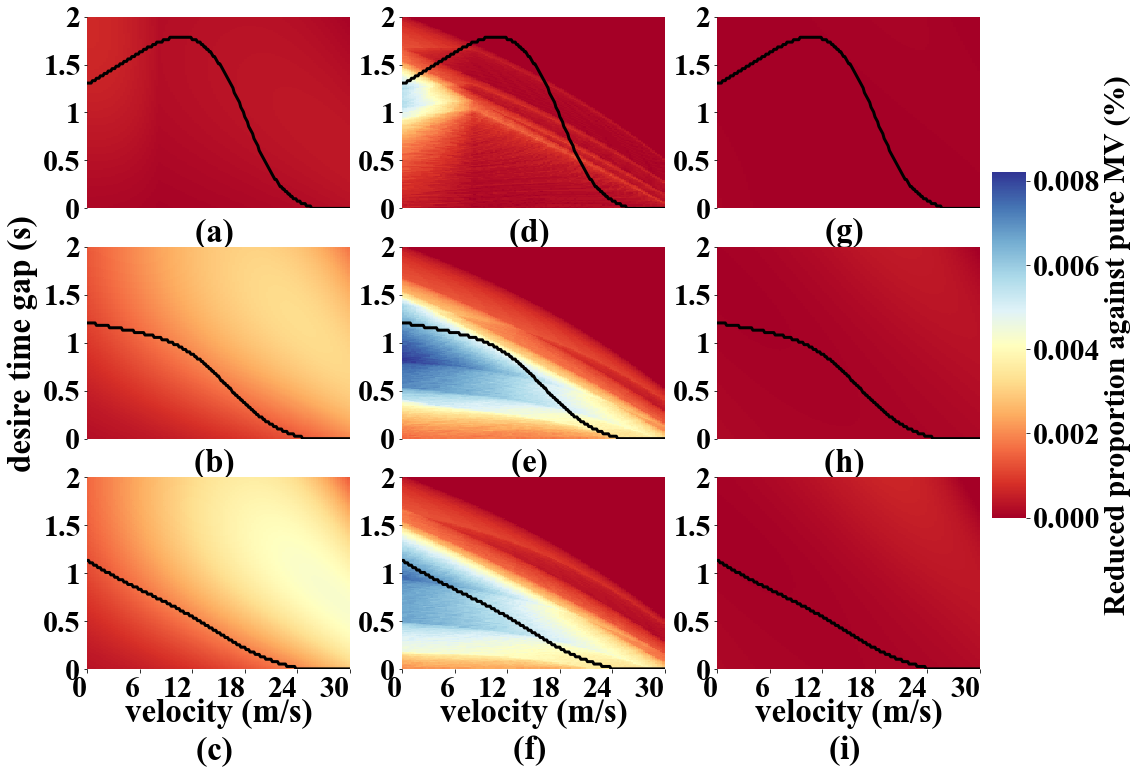
\includegraphics[width=9cm]{fig5.4_3.png}
  \caption{~Reduced proportion heatmaps of VOC among three IFTs against pure MV under three disturbances. (a)-(c) the case under disturbance \textit{Type \uppercase\expandafter{\romannumeral1}}; (d)-(f) the case under disturbance \textit{Type \uppercase\expandafter{\romannumeral2}}; (g)-(i) the case under disturbance \textit{Type \uppercase\expandafter{\romannumeral3}}. (a),(d),(g) The case of PF; (b),(e),(h) The case of PLF; (c),(f),(i) The case of MPLF.}
  \label{fig5.4_3}
\end{figure}




% From Fig.~\ref{Figure10} we can find that the CACCs can effectively reduce the emissions of various pollutants, and the magnitude of emission reduction of different emissions are also different. And different IFTs for the same pollutant can also cause significant differences. PLF and MPLF can cause a nearly 5-fold decrease in VOC relative to PF, while the impact of the three IFTs on reducing $CO_2$, PM, and $NO_x$ emissions are similar. In addition, the difference of PLF and MPLF on reducing the above four types of emissions are too negligible to distinguish which one is better compared to their volume.

Heatmaps demonstrate that the adoption of IFTs does reduce pollution emissions against pure MV, and the magnitude of emission reduction of different emissions are also different. As for VOC and CO2, the reduced proportion is less than 1.5\% in the whole control space under three types. For NOx, by contrast, the effect is significant as the reduced proportion is up to 7.8\% under disturbance \textit{Type \uppercase\expandafter{\romannumeral2}}.

From the perspective of the distribution of heatmaps in each subplot, Fig.~\ref{fig5.4_1} and Fig.~\ref{fig5.4_2} illustrate that the reduced proportion increases with the desire time gap and velocity for NOx and CO2. As for heatmaps in Fig.~\ref{fig5.4_3}, a different phenomenon is that the region can maintain lower emissions in the middle of control space, and the range of the area becomes smaller as the velocity increases.

From the perspective of differences between different disturbances, all pollutants show that IFTs can reduce pollutant emissions against pure MV under disturbance \textit{Type \uppercase\expandafter{\romannumeral1}} and disturbance \textit{Type \uppercase\expandafter{\romannumeral2}}, while is the same as MV under disturbance \textit{Type \uppercase\expandafter{\romannumeral3}}. Moreover, under disturbance \textit{Type \uppercase\expandafter{\romannumeral2}}, IFTs have the most significant impact on reducing pollutant emissions. From another perspective, adopting PF does not cause noteworthy differences compared to pure MV, while adopting PLF and MPLF can.

To summarize, although IFTs can only significantly reduce partial pollution emissions in the case of some types of disturbances, PLF and MPLF can substantially be superior to PF from the Eco-driving perspective in the three IFTs comparisons.



\subsection{Impact of actuation delay}

The actuation delay is another inevitable nature property of the actuators and sensors in the mechanical and control systems. According to relevant research, the stability analysis is also affected by the actuation delay as well as perception delays discussed before \citep{Xiao2008,Xiao2011,Wang2018}. Therefore, the string stability analyses of different IFTs considering the actuation delay are conducted in this paper. It should be clarified that the derivation of the stability conditions considering the actuation delay is also based on the PLF for simplicity.


By considering the actuation delay, the general form of PLF-abled CACCs is as follows:
\begin{equation}
  \begin{array}{l}
    \frac{{d{v_n}(t)}}{{dt}} = {g_n}\left( {{v_n}(t - {\tau ^*}),{s_n}(t - {\tau ^*}),\Delta {v_n}(t - {\tau ^*})} \right)                              \\
    \quad \quad \quad  + {\gamma _p}{g_{n - 1}}\left( {{v_{n - 1}}(t - {\tau ^*}),{s_{n - 1}}(t - {\tau ^*}),\Delta {v_{n - 1}}(t - {\tau ^*})} \right) \\
    \quad \quad \quad  + {\gamma _l}{g_1}\left( {{v_1}(t - {\tau ^*}),{s_1}(t - {\tau ^*}),\Delta {v_1}(t - {\tau ^*})} \right),
  \end{array}
  \label{eq_ac1}
\end{equation}
where ${\tau ^*} = \tau  + \eta $ denotes the full delay, including the perception delay and the actuation delay,  $\eta$ represents the actuation delay.

By introducing the small deviation of the velocity around the equilibrium state and the multiple reaction delays into Equation (\ref{eq_ac1}):
\begin{equation}
  \begin{array}{l}
    \frac{{d\delta {v_n}(t)}}{{dt}} = {g_n}\left( {v_n^e,s_n^e,0} \right) + {g_n}\left( {{v_n}(t - \tau _n^{{v^*}}),{s_n}\left( {t - \tau _n^{{s^*}}} \right),\Delta {v_n}\left( {t - \tau _n^{\Delta {v^*}}} \right)} \right)   \\
    \quad \quad \quad  + {\gamma _p}{g_{n - 1}}\left( {{v_{n - 1}}(t - \tau _{n - 1}^{{v^*}}),{s_{n - 1}}\left( {t - \tau _{n - 1}^{{v^*}}} \right),\Delta {v_{n - 1}}\left( {t - \tau _{n - 1}^{\Delta {v^*}}} \right)} \right) \\
    \quad \quad \quad  + {\gamma _l}{g_1}\left( {{v_1}(t - \tau _1^{{v^*}}),{s_1}\left( {t - \tau _1^v} \right),\Delta {v_1}\left( {t - \tau _1^{\Delta {v^*}}} \right)} \right),
  \end{array}
  \label{eq_ac2}
\end{equation}
where $\tau _n^{{v^*}} = \eta $, $\tau _n^{{s^*}} = \tau _n^s + \eta $, and $\tau _n^{\Delta {v^*}} = \tau _n^{\Delta v} + \eta $ represents the full delay of the velocity, gap, and velocity difference, respectively.

What needs to be mentioned is that Equation (\ref{Eq15}) and Equation (\ref{Eq16}) need to be extended to three-order to derive the corresponding conclusions in order to explore the impact of the actuation delay.

Adopting string stability analyses in Equation (\ref{Eq8})-Equation (\ref{Eq70}), the stability conditions considering both the perception delays and the actuation delay are as follows:
\begin{equation}
  \begin{array}{l}
    F_{PLF}^* =  - {\left( {g_n^v} \right)^2}g_n^{\Delta v}{\phi _1}^2 + {\left( {g_n^v} \right)^3}{\phi _1}{\phi _2} + {\left( {g_n^v} \right)^2}g_n^s{\phi _1}{\phi _3} - g_n^v{\left( {g_n^{\Delta v}} \right)^2}{\phi _1}^2 \\
    \quad \quad  - g_n^vg_n^{\Delta v}g_n^s{\phi _1}\left( {2{\phi _4} - {\phi _5}} \right) - g_n^v{\left( {g_n^s} \right)^2}\left( {{\phi _4}^2 + \frac{1}{2}{\phi _1}{\phi _6} - \frac{1}{2}{\phi _1}{\phi _8}} \right)       \\
    \quad \quad  - g_n^vg_n^s\left( {{\phi _7} + \frac{1}{2}{\phi _1}} \right) + {\left( {g_n^v} \right)^{ - 1}}{\left( {g_n^s} \right)^2} \ge 0,
  \end{array}
\end{equation}
where,
\begin{equation}
  \left\{ \begin{array}{l}
    {\phi _1} = \left( {1 + {\gamma _p} + {\gamma _l}} \right)                                                                                                                                                                                          \\
    {\phi _2} = ({\gamma _p} + \frac{{n\left( {n - 1} \right)}}{2}{\gamma _l})                                                                                                                                                                          \\
    {\phi _3} = \left( { - \frac{1}{2}\tau _n^{{v^*}} - \frac{1}{6}} \right) + {\gamma _p}\left( {\frac{1}{2}\tau _{n - 1}^{{v^*}} - \frac{7}{6}} \right) + {\gamma _l}\left( {\frac{{2n - 3}}{2}\tau _1^{{v^*}} - \frac{{3{n^2} - 3n + 1}}{6}} \right) \\
    {\phi _4} = \tau _n^{{s^*}} - \tau _n^{{v^*}} + {\gamma _p}\left( {\tau _{n - 1}^{{s^*}} - \tau _{n - 1}^{{v^*}}} \right) + {\gamma _l}\left( {\tau _1^{{s^*}} - \tau _1^{{v^*}}} \right)                                                           \\
    {\phi _5} = \tau _n^{\Delta {v^*}} + {\gamma _p}\tau _{n - 1}^{\Delta {v^*}} + {\gamma _l}\tau _1^{\Delta {v^*}}                                                                                                                                    \\
    {\phi _6} = {\left( {\tau _n^{{s^*}}} \right)^2} + {\gamma _p}{\left( {\tau _{n - 1}^{{s^*}}} \right)^2} + {\gamma _l}{\left( {\tau _1^{{s^*}}} \right)^2}                                                                                          \\
    {\phi _7} = {\gamma _p} + {\gamma _l}\left( {n - 1} \right)                                                                                                                                                                                         \\
    {\phi _8} = {\left( {\tau _n^{{v^*}}} \right)^2} + {\gamma _p}{\left( {\tau _{n - 1}^{{v^*}}} \right)^2} + {\gamma _l}{\left( {\tau _1^{{v^*}}} \right)^2}
  \end{array} \right.
\end{equation}

Besides, a corresponding head-to-tail string stability criterion can be derived \citep{ngoduy2013analytical,2009Heterogeneity}:
\begin{equation}
  \begin{array}{l}
    Q_{PLF}^* =  - {\left( {g_n^v} \right)^2}g_n^{\Delta v} + {\left( {g_n^v} \right)^2}g_n^s\left( { - \frac{1}{2}\tau _n^{{v^*}} - \frac{1}{6}} \right) - g_n^v{\left( {g_n^{\Delta v}} \right)^2}                               \\
    \quad \quad  - g_n^v{\left( {g_n^s} \right)^2}\left( {\frac{3}{2}{{\left( {\tau _n^{{s^*}}} \right)}^2} - 2\tau _n^{{s^*}}\tau _n^{{v^*}} + \frac{1}{2}{{\left( {\tau _n^{{v^*}}} \right)}^2}} \right) - \frac{1}{2}g_n^vg_n^s \\
    \quad \quad  - g_n^vg_n^{\Delta v}g_n^s\left( {2\tau _n^{{s^*}} - 2\tau _n^{{v^*}} - \tau _n^{\Delta {v^*}}} \right) + {\left( {g_n^v} \right)^{ - 1}}{\left( {g_n^s} \right)^2}                                               \\
    \quad \quad  + \left( {S - 1} \right)\left( { - {{\left( {g_n^v} \right)}^2}g_n^{\Delta v}{\phi _1}^2 + {{\left( {g_n^v} \right)}^3}{\phi _1}{\phi _2} + {{\left( {g_n^v} \right)}^2}g_n^s{\phi _1}{\phi _3}} \right.          \\
    \quad \quad  - g_n^v{\left( {g_n^{\Delta v}} \right)^2}{\phi _1}^2 - g_n^vg_n^{\Delta v}g_n^s{\phi _1}\left( {2{\phi _4} - {\phi _5}} \right) - g_n^vg_n^s\left( {{\phi _7} + \frac{1}{2}{\phi _1}} \right)                    \\
    \quad \quad \left. { - g_n^v{{\left( {g_n^s} \right)}^2}\left( {{\phi _4}^2 + \frac{1}{2}{\phi _1}{\phi _6} - \frac{1}{2}{\phi _1}{\phi _8}} \right) + {{\left( {g_n^v} \right)}^{ - 1}}{{\left( {g_n^s} \right)}^2}} \right)
  \end{array}
\end{equation}

For the sake of brevity of the paper, the process of deriving the head-to-tail string stability criterion is omitted. The expressions are as follows:
\begin{equation}
  \begin{array}{l}
    Q_{PF}^* =  - {\left( {g_n^v} \right)^2}g_n^{\Delta v} + {\left( {g_n^v} \right)^2}g_n^s\left( { - \frac{1}{2}\tau _n^{{v^*}} - \frac{1}{6}} \right) - g_n^v{\left( {g_n^{\Delta v}} \right)^2}                                                     \\
    \quad \quad  - g_n^v{\left( {g_n^s} \right)^2}\left( {\frac{3}{2}{{\left( {\tau _n^{{s^*}}} \right)}^2} - 2\tau _n^{{s^*}}\tau _n^{{v^*}} + \frac{1}{2}{{\left( {\tau _n^{{v^*}}} \right)}^2}} \right) - \frac{1}{2}g_n^vg_n^s                      \\
    \quad \quad  - g_n^vg_n^{\Delta v}g_n^s\left( {2\tau _n^{{s^*}} - 2\tau _n^{{v^*}} - \tau _n^{\Delta {v^*}}} \right) + {\left( {g_n^v} \right)^{ - 1}}{\left( {g_n^s} \right)^2}                                                                    \\
    \quad \quad  + \left( {S - 1} \right)\left( { - {{\left( {g_n^v} \right)}^2}g_n^{\Delta v}{\varepsilon _1}^2 + {{\left( {g_n^v} \right)}^3}{\varepsilon _1}{\gamma _p} + {{\left( {g_n^v} \right)}^2}g_n^s{\varepsilon _1}{\varepsilon _2}} \right. \\
    \quad \quad  - g_n^v{\left( {g_n^{\Delta v}} \right)^2}{\varepsilon _1}^2 - g_n^vg_n^{\Delta v}g_n^s{\varepsilon _1}\left( {2{\varepsilon _3} - {\varepsilon _4}} \right) - g_n^vg_n^s\left( {{\gamma _p} + \frac{1}{2}{\varepsilon _1}} \right)    \\
    \quad \quad \left. { - g_n^v{{\left( {g_n^s} \right)}^2}\left( {{\varepsilon _3}^2 + \frac{1}{2}{\varepsilon _1}{\varepsilon _5} - \frac{1}{2}{\varepsilon _1}{\varepsilon _6}} \right) + {{\left( {g_n^v} \right)}^{ - 1}}{{\left( {g_n^s} \right)}^2}} \right),
  \end{array}
\end{equation}
where,
\begin{equation}
  \left\{ \begin{array}{l}
    {\varepsilon _1} = 1 + {\gamma _p}                                                                                                                           \\
    {\varepsilon _2} = \left( { - \frac{1}{2}\tau _n^{{v^*}} - \frac{1}{6}} \right) + {\gamma _p}\left( {\frac{1}{2}\tau _{n - 1}^{{v^*}} - \frac{7}{6}} \right) \\
    {\varepsilon _3} = \tau _n^{{s^*}} - \tau _n^{{v^*}} + {\gamma _p}\left( {\tau _{n - 1}^{{s^*}} - \tau _{n - 1}^{{v^*}}} \right)                             \\
    {\varepsilon _4} = \tau _n^{\Delta {v^*}} + {\gamma _p}\tau _{n - 1}^{\Delta {v^*}}                                                                          \\
    {\varepsilon _5} = {\left( {\tau _n^{{s^*}}} \right)^2} + {\gamma _p}{\left( {\tau _{n - 1}^{{s^*}}} \right)^2}                                              \\
    {\varepsilon _6} = {\left( {\tau _n^{{v^*}}} \right)^2} + {\gamma _p}{\left( {\tau _{n - 1}^{{v^*}}} \right)^2}.
  \end{array} \right.
\end{equation}

\begin{equation}
  \begin{array}{l}
    Q_{MPLF}^* =  - {\left( {g_n^v} \right)^2}g_n^{\Delta v} + {\left( {g_n^v} \right)^2}g_n^s\left( { - \frac{1}{2}\tau _n^{{v^*}} - \frac{1}{6}} \right) - g_n^v{\left( {g_n^{\Delta v}} \right)^2}                                                                 \\
    \quad \quad  - g_n^v{\left( {g_n^s} \right)^2}\left( {\frac{3}{2}{{\left( {\tau _n^{{s^*}}} \right)}^2} - 2\tau _n^{{s^*}}\tau _n^{{v^*}} + \frac{1}{2}{{\left( {\tau _n^{{v^*}}} \right)}^2}} \right) - \frac{1}{2}g_n^vg_n^s                                    \\
    \quad \quad  - g_n^vg_n^{\Delta v}g_n^s\left( {2\tau _n^{{s^*}} - 2\tau _n^{{v^*}} - \tau _n^{\Delta {v^*}}} \right) + {\left( {g_n^v} \right)^{ - 1}}{\left( {g_n^s} \right)^2}                                                                                  \\
    \quad \quad  + \sum\limits_{n = 2}^S {\left[ {\left( { - {{\left( {g_n^v} \right)}^2}g_n^{\Delta v}{\vartheta _1}^2 + {{\left( {g_n^v} \right)}^3}{\vartheta _1}{\vartheta _2} + {{\left( {g_n^v} \right)}^2}g_n^s{\vartheta _1}{\vartheta _3}} \right.} \right.} \\
    \quad \quad  - g_n^v{\left( {g_n^{\Delta v}} \right)^2}{\vartheta _1}^2 - g_n^vg_n^{\Delta v}g_n^s{\vartheta _1}\left( {2{\vartheta _4} - {\vartheta _5}} \right) - g_n^vg_n^s\left( {{\vartheta _7} + \frac{1}{2}{\vartheta _1}} \right)                         \\
    \quad \quad \left. { - g_n^v{{\left( {g_n^s} \right)}^2}\left( {{\vartheta _4}^2 + \frac{1}{2}{\vartheta _1}{\vartheta _6} - \frac{1}{2}{\vartheta _1}{\vartheta _8}} \right) + {{\left( {g_n^v} \right)}^{ - 1}}{{\left( {g_n^s} \right)}^2}} \right],
  \end{array}
\end{equation}
where,
\begin{equation}
  \left\{ \begin{array}{l}
    {\vartheta _1} = 1 + \sum\limits_{k = 1}^{n - 1} {{\gamma _k}}                                                                                                                                                                                                                \\
    {\vartheta _2} = \sum\limits_{k = 1}^{n - 1} {\frac{{k\left( {k + 1} \right)}}{2}{\gamma _k}}                                                                                                                                                                                 \\
    {\vartheta _3} = \left( { - \frac{1}{2}\tau _n^{{v^*}} - \frac{1}{6}} \right) + \sum\limits_{k = 1}^{n - 1} {{\gamma _k}\left( {\frac{{{{\left( {k + 1} \right)}^2} - {k^2} - 2}}{2}\tau _{n - {\rm{k}}}^{{v^*}} - \frac{{{{\left( {k + 1} \right)}^3} - {k^3}}}{6}} \right)} \\
    {\vartheta _4} = \tau _n^{{s^*}} - \tau _n^{{v^*}} + \sum\limits_{k = 1}^{n - 1} {{\gamma _k}\left( {\tau _{n - k}^{{s^*}} - \tau _{n - {\rm{k}}}^{{v^*}}} \right)}                                                                                                           \\
    {\vartheta _5} = \tau _n^{\Delta {v^*}} + \sum\limits_{k = 1}^{n - 1} {{\gamma _k}\tau _{n - k}^{\Delta {v^*}}}                                                                                                                                                               \\
    {\vartheta _6} = {\left( {\tau _n^{{s^*}}} \right)^2} + \sum\limits_{k = 1}^{n - 1} {{\gamma _k}{{\left( {\tau _{n - k}^{{s^*}}} \right)}^2}}                                                                                                                                 \\
    {\vartheta _7} = \sum\limits_{k = 1}^{n - 1} {k{\gamma _k}}                                                                                                                                                                                                                   \\
    {\vartheta _8} = {\left( {\tau _n^{{v^*}}} \right)^2} + \sum\limits_{k = 1}^{n - 1} {{\gamma _k}{{\left( {\tau _{n - k}^{{v^*}}} \right)}^2}}.
  \end{array} \right.
\end{equation}

Moreover, to further explore the impact of the actuation delay on string stability, Fig.~\ref{fig_actuation_1} shows the heatmaps in control space (velocity-desire time gap), where color represents stability margin, and the black curve in each subfigure represents the margin stable curve. When the traffic flow environment and desire time gap setting is above the margin stable curve, it is string stable at equilibrium state, while the opposite represents the unstable traffic flow.

\begin{figure}
  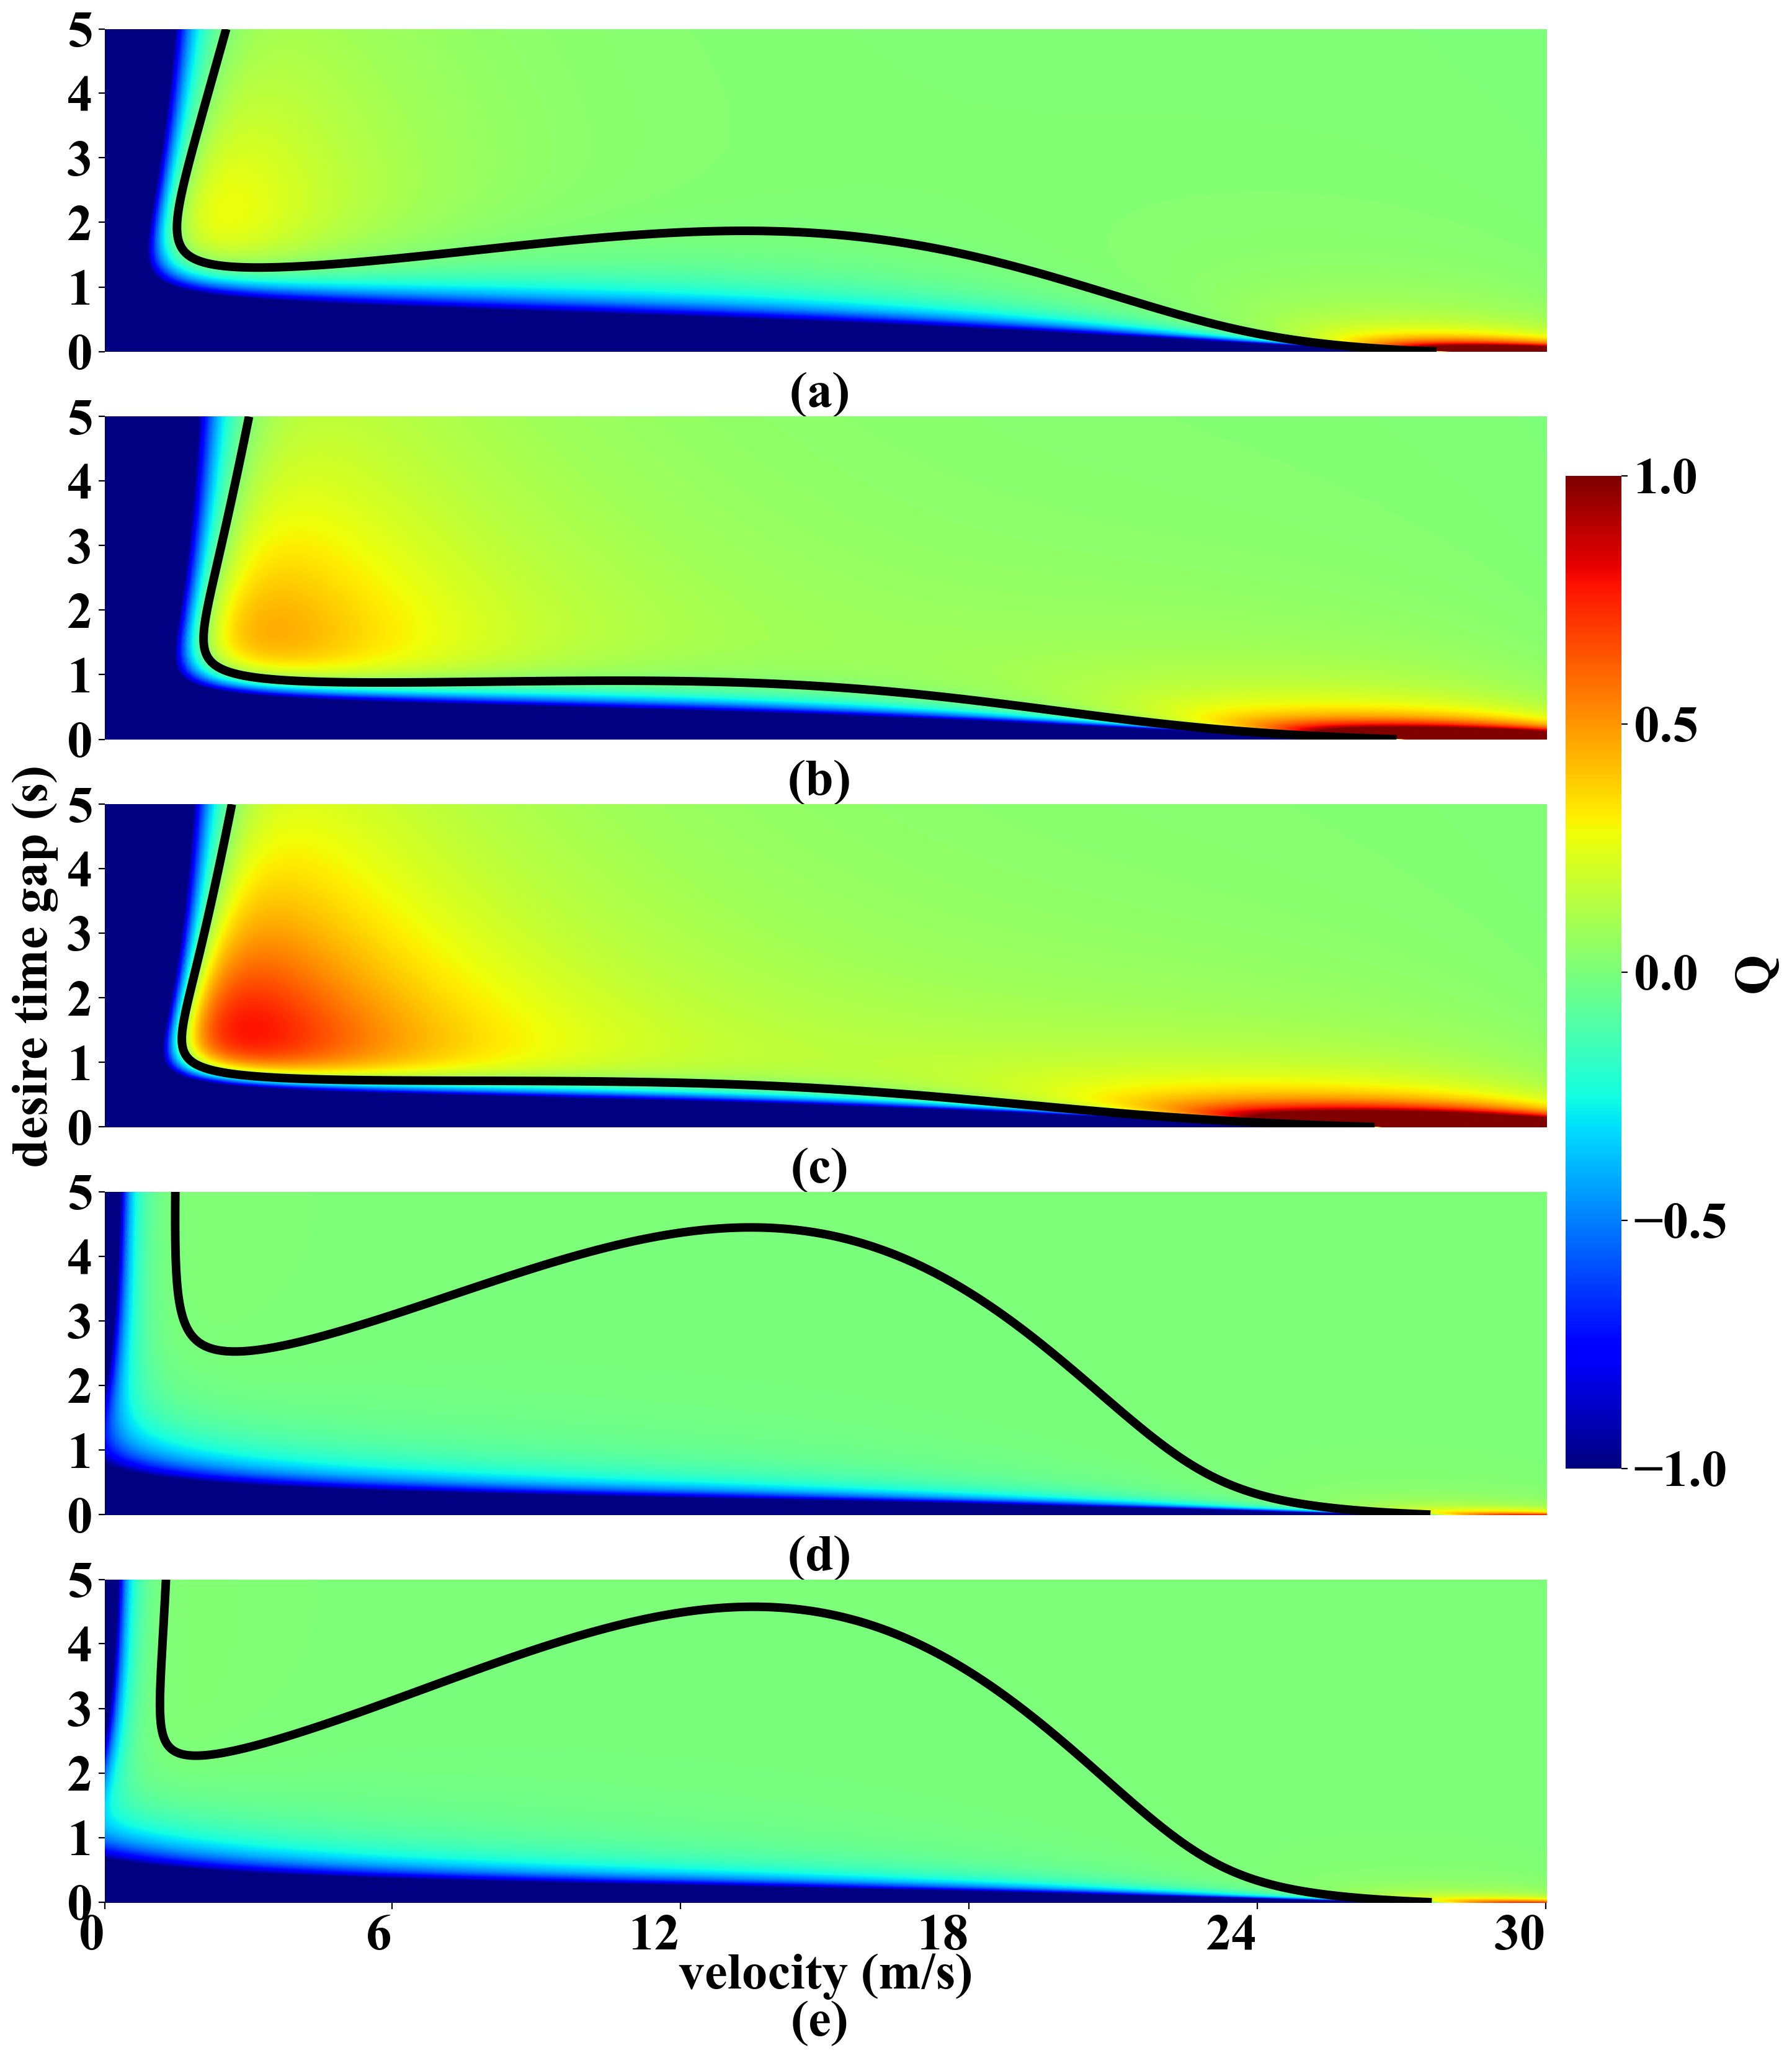
\includegraphics[width=9cm]{fig_actuation.png}
  \caption{~The heatmaps in the velocity-desire time gap of different IFTs. (a) the case of PF; (b) the case of PLF; (c) the case of MPLF; (d) the case of ACC; (e) the case of MV.}
  \label{fig_actuation_1}
\end{figure}

A phenomenon can be concluded from Fig.~\ref{fig_actuation_1} that the actuation delay deteriorates string stability, and this impact is even worse at low velocity. No matter what kind of vehicle control strategy, string stability is not guaranteed at speed velocity, even though the desire time gap is set to 5 s. Besides, this deterioration is exacerbated as the intensity of communication increases.

% When we look at the difference between different IFTs, we can find from Figure 11 that the reduction proportion improving effect of PLF and MPLF on VOC indicators is indistinguishable, while the impact of PF is less significant than the other two. Moreover, both PLF and MPLF can significantly reduce VOC in the area above the red curve, while the effect of PF in the whole area is less obvious. In addition, an interesting phenomenon can be found from figure 11 that a clear dividing line can be seen on the heatmap of all three IFTs, and the reduction proportion of the upper area of the dividing line can be significantly improved compared to that of the lower area. This phenomenon can be reasonably inferred that this boundary line is the critical line of pure MV performance degradation on VOC. The use of CAV can suppress the appearance of performance degradation, making this red line a crucial line for sudden changes in the reduction proportion. In addition, if we pay attention to the area below the red curve, we can find that the relative relationship between PF and PLF is also consistent with the conclusion in Fig.~\ref{Figure11}, while the case for PLF and MPLF are slightly different. The reduction proportion heat maps of PLF and MPLF maintain a similar trend overall, but when the desire time gap is in 0-0.3s , and the velocity is in 1-16m/s, it is obvious that PLF is better than MPLF.

% An example of a floating figure using the graphicx package.
% Note that \label must occur AFTER (or within) \caption.
% For figures, \caption should occur after the \includegraphics.
% Note that IEEEtran v1.7 and later has special internal code that
% is designed to preserve the operation of \label within \caption
% even when the captionsoff option is in effect. However, because
% of issues like this, it may be the safest practice to put all your
% \label just after \caption rather than within \caption{}.
%
% Reminder: the "draftcls" or "draftclsnofoot", not "draft", class
% option should be used if it is desired that the figures are to be
% displayed while in draft mode.
%
%\begin{figure}[!t]
%\centering
%\includegraphics[width=2.5in]{myfigure}
% where an .eps filename suffix will be assumed under latex, 
% and a .pdf suffix will be assumed for pdflatex; or what has been declared
% via \DeclareGraphicsExtensions.
%\caption{Simulation results for the network.}
%\label{fig_sim}
%\end{figure}

% Note that the IEEE typically puts floats only at the top, even when this
% results in a large percentage of a column being occupied by floats.


% An example of a double column floating figure using two subfigures.
% (The subfig.sty package must be loaded for this to work.)
% The subfigure \label commands are set within each subfloat command,
% and the \label for the overall figure must come after \caption.
% \hfil is used as a separator to get equal spacing.
% Watch out that the combined width of all the subfigures on a 
% line do not exceed the text width or a line break will occur.
%
%\begin{figure*}[!t]
%\centering
%\subfloat[Case I]{\includegraphics[width=2.5in]{box}%
%\label{fig_first_case}}
%\hfil
%\subfloat[Case II]{\includegraphics[width=2.5in]{box}%
%\label{fig_second_case}}
%\caption{Simulation results for the network.}
%\label{fig_sim}
%\end{figure*}
%
% Note that often IEEE papers with subfigures do not employ subfigure
% captions (using the optional argument to \subfloat[]), but instead will
% reference/describe all of them (a), (b), etc., within the main caption.
% Be aware that for subfig.sty to generate the (a), (b), etc., subfigure
% labels, the optional argument to \subfloat must be present. If a
% subcaption is not desired, just leave its contents blank,
% e.g., \subfloat[].


% An example of a floating table. Note that, for IEEE style tables, the
% \caption command should come BEFORE the table and, given that table
% captions serve much like titles, are usually capitalized except for words
% such as a, an, and, as, at, but, by, for, in, nor, of, on, or, the, to
% and up, which are usually not capitalized unless they are the first or
% last word of the caption. Table text will default to \footnotesize as
% the IEEE normally uses this smaller font for tables.
% The \label must come after \caption as always.
%
%\begin{table}[!t]
%% increase table row spacing, adjust to taste
%\renewcommand{\arraystretch}{1.3}
% if using array.sty, it might be a good idea to tweak the value of
% \extrarowheight as needed to properly center the text within the cells
%\caption{An Example of a Table}
%\label{table_example}
%\centering
%% Some packages, such as MDW tools, offer better commands for making tables
%% than the plain LaTeX2e tabular which is used here.
%\begin{tabular}{|c||c|}
%\hline
%One & Two\\
%\hline
%Three & Four\\
%\hline
%\end{tabular}
%\end{table}


% Note that the IEEE does not put floats in the very first column
% - or typically anywhere on the first page for that matter. Also,
% in-text middle ("here") positioning is typically not used, but it
% is allowed and encouraged for Computer Society conferences (but
% not Computer Society journals). Most IEEE journals/conferences use
% top floats exclusively. 
% Note that, LaTeX2e, unlike IEEE journals/conferences, places
% footnotes above bottom floats. This can be corrected via the
% \fnbelowfloat command of the stfloats package.




\section{Conclusion}
\label{Section 6}
This paper designed the platoon management for CACC strings that formed several platoons due to the limitation of the C-V2X communication range. The model of CACC was firstly proposed based on specific IFTs, and multiple time delays were considered in the design of the general model. To select model parameters, corresponding linear string stability analyses were implemented to obtain the stability condition against a slight disturbance under the open boundary condition. Then, numerical analyses and simulations were carried out to verify the stability region based on the CACC platoon controller from the perspective of long-wave and short-wave stability. Finally, the differences of different IFTs in stability region, robustness, safety, and emission were explored to determine the effect of the CACC platoon controllers based on different IFTs. The following conclusions can be drawn through theoretical analysis:
\begin{enumerate}
  \item The string stability criterion of the CACC platoon controller indicates that the linear stability is directly related to equilibrium velocity.
  \item As the equilibrium velocity increases, the margin stable curve of ACC, MV, and PF will have a peak, which indicates that it is difficult for ACC to maintain stability when the equilibrium velocity is low, and the CACC platoon controller based on PLF and MPLF can directly inhibit the emergence of this peak.
  \item CACC platoon controller based on IFTs can maintain a smaller desire time gap than ACC and MV without losing stability with appropriate control parameters, indicating a significant traffic capacity and safety gain via communication.
  \item With the increase of the control parameters of the CACC platoon controller, the margin stable curve of the desire time gap decreases, but the decline will be smaller and smaller. Therefore, it is not necessary to set control parameters to high values. The recommended control parameter is $\gamma_p=\gamma_l=0.3$ because the gain of the desire time gap has a diminished marginal effect with a further increase of parameters.
  \item By comparing the effects of different IFTs from the four perspectives of stability, robustness, safety, and emission, we can find that PLF and MPLF can maintain a significant improvement compared to PF. Still, the difference between the two is not apparent. MPLF can keep a slight advantage in stability region, safety, and emissions, while PLF is better in robustness. However, MPLF requires an ideal communication environment that leads to exponential pressure on communication bandwidth. Its gain relative to PLF may need to be considered in a balanced manner. In general, with higher communication bandwidth or fewer communication vehicles, MPLF will be a better option; on the contrary, PLF is more suitable.
\end{enumerate}





% if have a single appendix:
%\appendix[Proof of the Zonklar Equations]
% or
%\appendix % for no appendix heading
% do not use \section anymore after \appendix, only \section*
% is possibly needed

% use appendices with more than one appendix
% then use \section to start each appendix
% you must declare a \section before using any
% \subsection or using \label (\appendices by itself
% starts a section numbered zero.)
%


% \appendices
% \section{Proof of the First Zonklar Equation}
% Appendix one text goes here.

% you can choose not to have a title for an appendix
% if you want by leaving the argument blank
% \section{}
% Appendix two text goes here.


\section*{Acknowledgment}


This work was sponsored by the National Science Foundation of China (No. 51878161 and No.52072067) and the China Postdoctoral Science Foundation (No.2020M681466).




\appendix
\section*{Appendix A. Platoon management strategy}
\label{appendix1}
Here we explain in detail why platoon management strategy is adopted and how it works.

As the standard communication protocol for CACCs selected by the Federal Communications Commission (FCC), C-V2X is significantly superior to Dedicated Short-Range Communications (DSRC) in terms of communication distance and delay. However, C-V2X is still limited by the communication bandwidth because the communication bandwidth of the C-V2X is also 20MHz same as the DSRC \citep{Boubakri2020,Chen2020,Nardini2018}. This means that the limit of channel occupancy is 20MHz, and the larger the Channel Busy Ratio (CBR), the worse the environment for communication. The impact of this limitation on the CACC platoons is that CACC platoons cannot be expanded indefinitely. Moreover, if the CBR is high, it will lead to severe Packet Error Rate (PER) and Information Age (IA), which indicates unreliable communication. As a result, all CACCs in the platoon will be forced to degrade to ACCs to avoid errors or delays in communication \citep{Vukadinovic2018,Vu2020}. It is worth noting that the feasibility of IFTs mentioned in this paper is demonstrated in the relevant literature \citep{zheng2015stability,Martin-Sacristan2020,Thota2019,Pirani2022}.

However, according to relevant research, ACCs cannot significantly benefit traffic flow stability and capacity, while CACCs can \citep{Shang2021,Shladover2012,Nikolos2015}. Based on the above analysis, we can conclude that the benefits of CACCs can be maintained by ensuring CACCs do not degrade to ACCs as many as possible. A corresponding platoon management strategy is proposed.


According to the platoon management strategy, the first CACC beyond the maximum platoon size will automatically degrade to a leader ACC that does not accept information and only broadcasts its information. Moreover, local platoons are generated by decomposing the long platoon with the leader ACCs as the leaders of local platoons. Different local platoons apply channel scheduling methods and communicate in different channels to avoid the harsh communication environment caused by all CACCs communicating on the same channel. Based on this strategy, although the communication gain of some CACCs is sacrificed, most CACCs cannot degrade to ACCs. Thus, the benefits of CACCs on traffic flow stability and traffic capacity can be maintained under this strategy.

It is worth noting that the maximum platoon size S mentioned here can be calculated by the actual maximum C-V2X communication bandwidth and packet size. For convenience, we chose the maximum platoon size S=5 for simulation. Moreover, according to the report on the fourteenth meeting of IMT-2020 (5G) Promotion Group Cellular-Vehicle-to-everything Working Group, communication can maintain less than 47.58ms of delay, 3.12\% PER, and 38.62\% CBR with 54 OBUs within a 100m radius, under 10MHz channel bandwidth. This communication environment is sufficient to guarantee the platoon communicates properly under the platoon management strategy.


% Can use something like this to put references on a page
% by themselves when using endfloat and the captionsoff option.
\ifCLASSOPTIONcaptionsoff
  \newpage
\fi



% trigger a \newpage just before the given reference
% number - used to balance the columns on the last page
% adjust value as needed - may need to be readjusted if
% the document is modified later
%\IEEEtriggeratref{8}
% The "triggered" command can be changed if desired:
%\IEEEtriggercmd{\enlargethispage{-5in}}

% references section
% can use a bibliography generated by BibTeX as a .bbl file
% BibTeX documentation can be easily obtained at:
% http://mirror.ctan.org/biblio/bibtex/contrib/doc/
% The IEEEtran BibTeX style support page is at:
% http://www.michaelshell.org/tex/ieeetran/bibtex/
\bibliographystyle{IEEEtran}
% argument is your BibTeX string definitions and bibliography database(s)
%\bibliography{IEEEabrv,../bib/paper}
%\bibliography{cas-refs}
% <OR> manually copy in the resultant .bbl file
% set second argument of \begin to the number of references
% (used to reserve space for the reference number labels box)

\bibliography{ref}
% \begin{thebibliography}{34}
% \providecommand{\natexlab}[1]{#1}
% \providecommand{\url}[1]{\texttt{#1}}
% \expandafter\ifx\csname urlstyle\endcsname\relax
%   \providecommand{\doi}[1]{doi: #1}\else
%   \providecommand{\doi}{doi: \begingroup \urlstyle{rm}\Url}\fi

% \bibitem[Wang et~al.(2019)Wang, Bian, Shladover, Wu, Li, and
%   Barth]{wang2019survey}
% Ziran Wang, Yougang Bian, Steven~E Shladover, Guoyuan Wu, Shengbo~Eben Li, and
%   Matthew~J Barth.
% \newblock A survey on cooperative longitudinal motion control of multiple
%   connected and automated vehicles.
% \newblock \emph{IEEE Intelligent Transportation Systems Magazine}, 12\penalty0
%   (1):\penalty0 4--24, 2019.

% \bibitem[Shladover et~al.(2015)Shladover, Nowakowski, Lu, and
%   Ferlis]{shladover2015cooperative}
% Steven~E Shladover, Christopher Nowakowski, Xiao-Yun Lu, and Robert Ferlis.
% \newblock Cooperative adaptive cruise control: Definitions and operating
%   concepts.
% \newblock \emph{Transportation Research Record}, 2489\penalty0 (1):\penalty0
%   145--152, 2015.

% \bibitem[Wang et~al.(2020{\natexlab{b}})Wang, Zheng, Xu, Wang, and
%   Li]{wang2020controllability}
% Jiawei Wang, Yang Zheng, Qing Xu, Jianqiang Wang, and Keqiang Li.
% \newblock Controllability analysis and optimal control of mixed traffic flow
%   with human-driven and autonomous vehicles.
% \newblock \emph{IEEE Transactions on Intelligent Transportation Systems},
%   2020{\natexlab{b}}.

% \bibitem[Hall and Chin(2005)]{hall2005vehicle}
% Randolph Hall and Chinan Chin.
% \newblock Vehicle sorting for platoon formation: Impacts on highway entry and
%   throughput.
% \newblock \emph{Transportation Research Part C: Emerging Technologies},
%   13\penalty0 (5-6):\penalty0 405--420, 2005.


% \bibitem[Yanyan~Qin(2021)]{qin2021LWR}
% Daiheng~Ni Yanyan~Qin, Hao~Wang.
% \newblock Lwr model for traffic flow mixed with cacc vehicles.
% \newblock \emph{Transportation Science}, 2021.

% \bibitem[Zhou et~al.(2021)Zhou, Ruan, Ma, Dong, and Wang]{zhou2021impact}
% Linjie Zhou, Tiancheng Ruan, Ke~Ma, Changyin Dong, and Hao Wang.
% \newblock Impact of cav platoon management on traffic flow considering
%   degradation of control mode.
% \newblock \emph{Physica A: Statistical Mechanics and its Applications}, page
%   126193, 2021.

% \bibitem[Zhang et~al.(2020)Zhang, Bai, Hu, and Wang]{zhang2020control}
% Yu~Zhang, Yu~Bai, Jia Hu, and Meng Wang.
% \newblock Control design, stability analysis, and traffic flow implications for
%   cooperative adaptive cruise control systems with compensation of
%   communication delay.
% \newblock \emph{Transportation Research Record}, 2674\penalty0 (8):\penalty0
%   638--652, 2020.


% \bibitem[Navas and Milan{\'e}s(2019)]{navas2019mixing}
% Francisco Navas and Vicente Milan{\'e}s.
% \newblock Mixing v2v-and non-v2v-equipped vehicles in car following.
% \newblock \emph{Transportation research part C: emerging technologies},
%   108:\penalty0 167--181, 2019.

% \bibitem[Wang et~al.(2020{\natexlab{a}})Wang, Gong, Zhou, Li, and
%   Peeta]{wang2020cooperative}
% Chaojie Wang, Siyuan Gong, Anye Zhou, Tao Li, and Srinivas Peeta.
% \newblock Cooperative adaptive cruise control for connected autonomous vehicles
%   by factoring communication-related constraints.
% \newblock \emph{Transportation Research Part C: Emerging Technologies},
%   113:\penalty0 124--145, 2020{\natexlab{a}}.

% \bibitem[Li et~al.(2020)Li, Bian, Li, Xu, and Wang]{li2020distributed}
% Keqiang Li, Yougang Bian, Shengbo~Eben Li, Biao Xu, and Jianqiang Wang.
% \newblock Distributed model predictive control of multi-vehicle systems with
%   switching communication topologies.
% \newblock \emph{Transportation Research Part C: Emerging Technologies},
%   118:\penalty0 102717, 2020.

% \bibitem[Zhou et~al.(2020)Zhou, Gong, Wang, and Peeta]{zhou2020smooth}
% Anye Zhou, Siyuan Gong, Chaojie Wang, and Srinivas Peeta.
% \newblock Smooth-switching control-based cooperative adaptive cruise control by
%   considering dynamic information flow topology.
% \newblock \emph{Transportation Research Record}, 2674\penalty0 (4):\penalty0
%   444--458, 2020.

% \bibitem[Zheng et~al.(2015)Zheng, Li, Wang, Cao, and Li]{zheng2015stability}
% Yang Zheng, Shengbo~Eben Li, Jianqiang Wang, Dongpu Cao, and Keqiang Li.
% \newblock Stability and scalability of homogeneous vehicular platoon: Study on
%   the influence of information flow topologies.
% \newblock \emph{IEEE Transactions on intelligent transportation systems},
%   17\penalty0 (1):\penalty0 14--26, 2015.

% \bibitem[Jia et~al.(2015)Jia, Lu, Wang, Zhang, and Shen]{jia2015survey}
% Dongyao Jia, Kejie Lu, Jianping Wang, Xiang Zhang, and Xuemin Shen.
% \newblock A survey on platoon-based vehicular cyber-physical systems.
% \newblock \emph{IEEE communications surveys \& tutorials}, 18\penalty0
%   (1):\penalty0 263--284, 2015.

% \bibitem[Ma et~al.(2020)Ma, Wang, Yang, Wu, Zhu, Gelbal, Aksun-Guvenc, and
%   Guvenc]{ma2020stability}
% Fangwu Ma, Jiawei Wang, Yu~Yang, Liang Wu, Sheng Zhu, Sukru~Yaren Gelbal, Bilin
%   Aksun-Guvenc, and Levent Guvenc.
% \newblock Stability design for the homogeneous platoon with communication time
%   delay.
% \newblock \emph{Automotive Innovation}, 3:\penalty0 101--110, 2020.

% \bibitem[Zheng et~al.(2014)Zheng, Li, Wang, Li, et~al.]{zheng2014influence}
% Yang Zheng, Shengbo~Eben Li, Jianqiang Wang, Keqiang Li, et~al.
% \newblock Influence of information flow topology on closed-loop stability of
%   vehicle platoon with rigid formation.
% \newblock In \emph{17th International IEEE Conference on Intelligent
%   Transportation Systems (ITSC)}, pages 2094--2100. IEEE, 2014.

% \bibitem[Farah and Koutsopoulos(2014)]{farah2014cooperative}
% Haneen Farah and Haris~N Koutsopoulos.
% \newblock Do cooperative systems make drivers’ car-following behavior safer?
% \newblock \emph{Transportation research part C: emerging technologies},
%   41:\penalty0 61--72, 2014.

% \bibitem[Yu and Shi(2015)]{yu2015effects}
% Shaowei Yu and Zhongke Shi.
% \newblock The effects of vehicular gap changes with memory on traffic flow in
%   cooperative adaptive cruise control strategy.
% \newblock \emph{Physica A: Statistical Mechanics and its Applications},
%   428:\penalty0 206--223, 2015.

% \bibitem[Li et~al.(2015)Li, Li, Xu, and Qian]{li2015stability}
% Zhipeng Li, Wenzhong Li, Shangzhi Xu, and Yeqing Qian.
% \newblock Stability analysis of an extended intelligent driver model and its
%   simulations under open boundary condition.
% \newblock \emph{Physica A: Statistical Mechanics and its Applications},
%   419:\penalty0 526--536, 2015.

% \bibitem[Fernandes and Nunes(2014)]{fernandes2014multiplatooning}
% Pedro Fernandes and Urbano Nunes.
% \newblock Multiplatooning leaders positioning and cooperative behavior
%   algorithms of communicant automated vehicles for high traffic capacity.
% \newblock \emph{IEEE Transactions on Intelligent Transportation Systems},
%   16\penalty0 (3):\penalty0 1172--1187, 2014.

% \bibitem[Milan{\'e}s and Shladover(2014)]{milanes2014modeling}
% Vicente Milan{\'e}s and Steven~E Shladover.
% \newblock Modeling cooperative and autonomous adaptive cruise control dynamic
%   responses using experimental data.
% \newblock \emph{Transportation Research Part C: Emerging Technologies},
%   48:\penalty0 285--300, 2014.

% \bibitem[Milan{\'e}s et~al.(2013)Milan{\'e}s, Shladover, Spring, Nowakowski,
%   Kawazoe, and Nakamura]{milanes2013cooperative}
% Vicente Milan{\'e}s, Steven~E Shladover, John Spring, Christopher Nowakowski,
%   Hiroshi Kawazoe, and Masahide Nakamura.
% \newblock Cooperative adaptive cruise control in real traffic situations.
% \newblock \emph{IEEE Transactions on intelligent transportation systems},
%   15\penalty0 (1):\penalty0 296--305, 2013.

% \bibitem[Dey et~al.(2015)Dey, Yan, Wang, Wang, Shen, Chowdhury, Yu, Qiu, and
%   Soundararaj]{dey2015review}
% Kakan~C Dey, Li~Yan, Xujie Wang, Yue Wang, Haiying Shen, Mashrur Chowdhury, Lei
%   Yu, Chenxi Qiu, and Vivekgautham Soundararaj.
% \newblock A review of communication, driver characteristics, and controls
%   aspects of cooperative adaptive cruise control (cacc).
% \newblock \emph{IEEE Transactions on Intelligent Transportation Systems},
%   17\penalty0 (2):\penalty0 491--509, 2015.

% \bibitem[Ngoduy(2013)]{ngoduy2013analytical}
% Dong Ngoduy.
% \newblock Analytical studies on the instabilities of heterogeneous intelligent
%   traffic flow.
% \newblock \emph{Communications in Nonlinear Science and Numerical Simulation},
%   18\penalty0 (10):\penalty0 2699--2706, 2013.

% \bibitem[Yao et~al.(2021)Yao, Xu, Jiang, and Hu]{yao2021linear}
% Zhihong Yao, Taorang Xu, Yangsheng Jiang, and Rong Hu.
% \newblock Linear stability analysis of heterogeneous traffic flow considering
%   degradations of connected automated vehicles and reaction time.
% \newblock \emph{Physica A: Statistical Mechanics and its Applications},
%   561:\penalty0 125218, 2021.

% \bibitem[Jin and Orosz(2014)]{jin2014dynamics}
% I~Ge Jin and G{\'a}bor Orosz.
% \newblock Dynamics of connected vehicle systems with delayed acceleration
%   feedback.
% \newblock \emph{Transportation Research Part C: Emerging Technologies},
%   46:\penalty0 46--64, 2014.

% \bibitem[Sun et~al.(2018)Sun, Zheng, and Sun]{sun2018stability}
% Jie Sun, Zuduo Zheng, and Jian Sun.
% \newblock Stability analysis methods and their applicability to car-following
%   models in conventional and connected environments.
% \newblock \emph{Transportation research part B: methodological}, 109:\penalty0
%   212--237, 2018.

% \bibitem[Chang et~al.(2020)Chang, Li, Rong, Zhao, et~al.]{chang2020analysis}
% Xin Chang, Haijian Li, Jian Rong, Xiaohua Zhao, et~al.
% \newblock Analysis on traffic stability and capacity for mixed traffic flow
%   with platoons of intelligent connected vehicles.
% \newblock \emph{Physica A: Statistical Mechanics and its Applications},
%   557:\penalty0 124829, 2020.

% \bibitem[Li et~al.(2017)Li, Wang, Wang, Xing, Liu, and Wei]{li2017evaluation}
% Ye~Li, Hao Wang, Wei Wang, Lu~Xing, Shanwen Liu, and Xueyan Wei.
% \newblock Evaluation of the impacts of cooperative adaptive cruise control on
%   reducing rear-end collision risks on freeways.
% \newblock \emph{Accident Analysis \& Prevention}, 98:\penalty0 87--95, 2017.

% \bibitem[Kesting et~al.(2008)Kesting, Treiber, Sch{\"o}nhof, and
%   Helbing]{kesting2008adaptive}
% Arne Kesting, Martin Treiber, Martin Sch{\"o}nhof, and Dirk Helbing.
% \newblock Adaptive cruise control design for active congestion avoidance.
% \newblock \emph{Transportation Research Part C: Emerging Technologies},
%   16\penalty0 (6):\penalty0 668--683, 2008.

% \bibitem[Kesting et~al.(2007)Kesting, Treiber, Sch{\"o}nhof, Kranke, and
%   Helbing]{kesting2007jam}
% Arne Kesting, Martin Treiber, Martin Sch{\"o}nhof, Florian Kranke, and Dirk
%   Helbing.
% \newblock Jam-avoiding adaptive cruise control (acc) and its impact on traffic
%   dynamics.
% \newblock In \emph{Traffic and Granular Flow’05}, pages 633--643. Springer,
%   2007.

% \bibitem[Hafeez et~al.(2013)Hafeez, Zhao, Ma, and Mark]{hafeez2013performance}
% Khalid~Abdel Hafeez, Lian Zhao, Bobby Ma, and Jon~W Mark.
% \newblock Performance analysis and enhancement of the dsrc for vanet's safety
%   applications.
% \newblock \emph{IEEE Transactions on Vehicular Technology}, 62\penalty0
%   (7):\penalty0 3069--3083, 2013.

% \bibitem[Gong et~al.(2016)Gong, Shen, and Du]{gong2016constrained}
% Siyuan Gong, Jinglai Shen, and Lili Du.
% \newblock Constrained optimization and distributed computation based car
%   following control of a connected and autonomous vehicle platoon.
% \newblock \emph{Transportation Research Part B: Methodological}, 94:\penalty0
%   314--334, 2016.

% \bibitem[Li et~al.(2014)Li, Cui, An, and Parsafard]{li2014stop}
% Xiaopeng Li, Jianxun Cui, Shi An, and Mohsen Parsafard.
% \newblock Stop-and-go traffic analysis: Theoretical properties, environmental
%   impacts and oscillation mitigation.
% \newblock \emph{Transportation Research Part B: Methodological}, 70:\penalty0
%   319--339, 2014.

% \bibitem[Panis et~al.(2006)Panis, Broekx, and Liu]{panis2006modelling}
% Luc~Int Panis, Steven Broekx, and Ronghui Liu.
% \newblock Modelling instantaneous traffic emission and the influence of traffic
%   speed limits.
% \newblock \emph{Science of the total environment}, 371\penalty0 (1-3):\penalty0
%   270--285, 2006.

% \end{thebibliography}

\begin{IEEEbiography}[{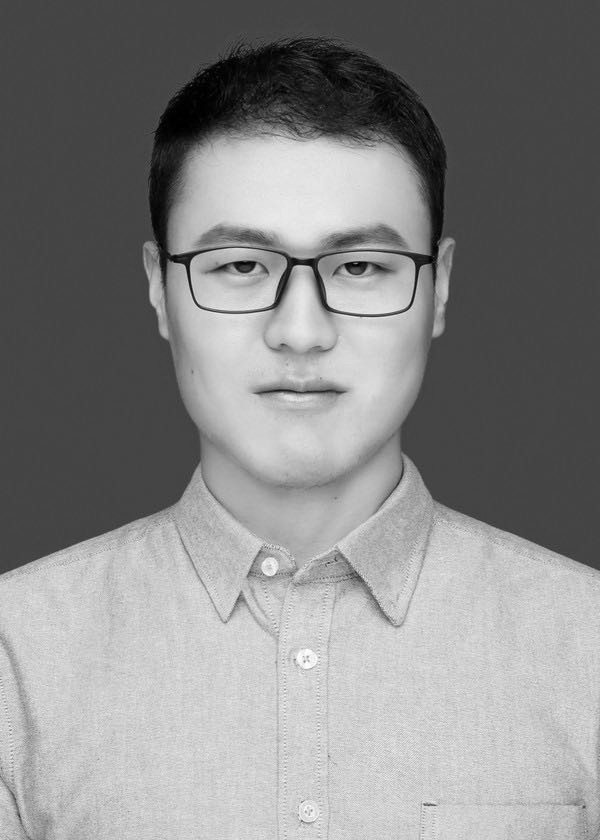
\includegraphics[width=1in,height=1.25in,clip,keepaspectratio]{ruan_bio}}]{Tiancheng Ruan}
  received the B.Eng. degrees in transportation planning and management from Chang'an University, Xi'an, China, in 2019. He is currently pursuing the Ph.D. degree with School of Transportation in Southeast University. His research interests include traffic flow theory, intelligent transportation systems, and stability analyses.
\end{IEEEbiography}

\begin{IEEEbiography}[{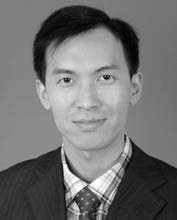
\includegraphics[width=1in,height=1.25in,clip,keepaspectratio]{wang_bio}}]{Hao Wang}
  received the M.Eng. and Ph.D. degrees in transportation engineering from Southeast University, Nanjing, China, in 2002 and 2008, respectively. He is currently a Professor with school of transportation, Southeast University. He is also the Deputy Director of the Jiangsu Key Laboratory of Urban Intelligent Transportation Systems, and a member of the National Transportation Modeling and Simulation Association. His research interests include traffic flow theory, traffic control and traffic simulation.
\end{IEEEbiography}

\begin{IEEEbiography}[{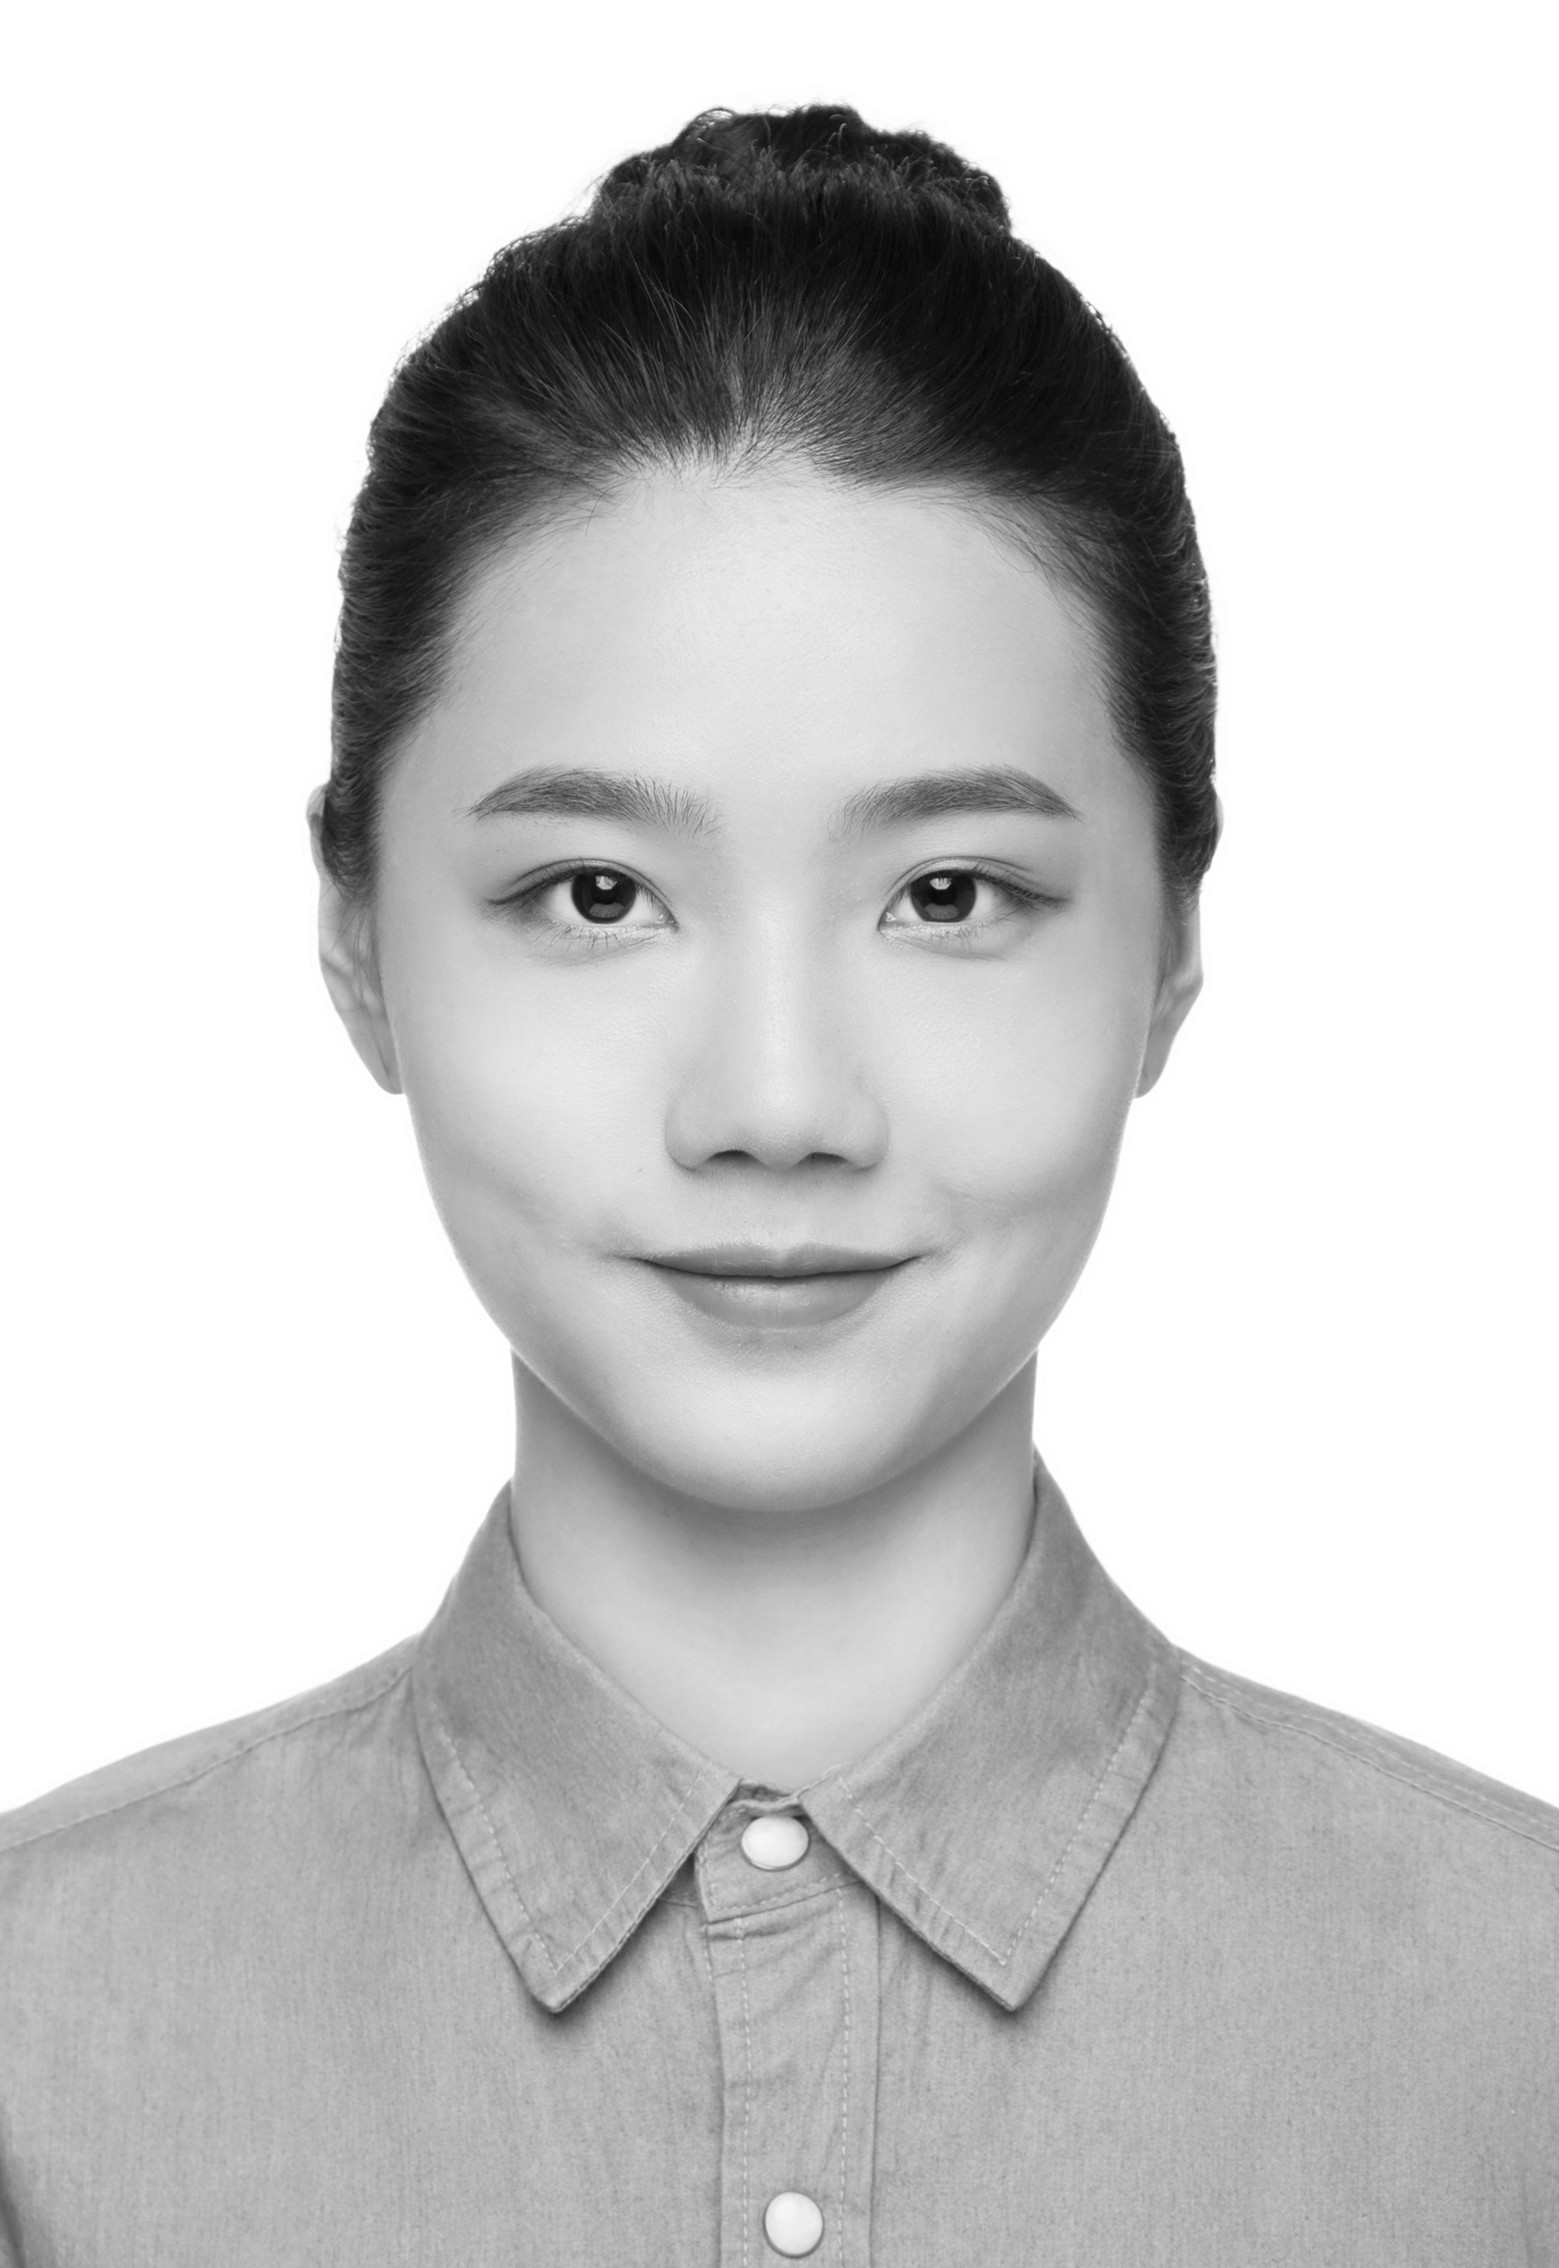
\includegraphics[width=1in,height=1.25in,clip,keepaspectratio]{zhou_bio}}]{Linjie Zhou}
  received the B.Eng. degrees in transportation planning and management from Southeast University, Nanjing, China, in 2019. She is currently pursuing the B.S. degree with the Jiangsu Province Collaborative Innovation Center of Modern Urban Traffic Technologies, School of Transportation. Her research interests include traffic flow theory, intelligent transportation systems, and microscopic simualtion.
\end{IEEEbiography}

\begin{IEEEbiography}[{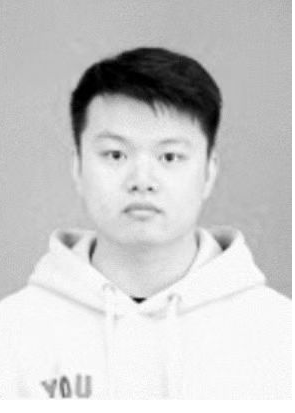
\includegraphics[width=1in,height=1.25in,clip,keepaspectratio]{zhang_bio}}]{Yantang Zhang}
  received the MA.Eng. and MA degrees in transportation planning and management from Harbin Institute of technology University, Harbin, China in 2019 and 2021, respectively, where he is currently pursuing the Ph.D. degree. His research interests include spatio-temporal relationship between travel behavior and built environment, traffic safety et al.
\end{IEEEbiography}

\begin{IEEEbiography}[{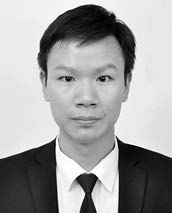
\includegraphics[width=1in,height=1.25in,clip,keepaspectratio]{dong_bio}}]{Changyin Dong}
  received the B.S. and Ph.D. degrees in transportation planning and management from Southeast University, Nanjing, China, in 2014 and 2020, respectively. He is currently working as a postdoctoral fellow with the Jiangsu Province Collaborative Innovation Center of Modern Urban Traffic Technologies, Southeast University. His research interests include traffic flow theory, intelligent transportation systems and automated vehicle control.
\end{IEEEbiography}

\begin{IEEEbiography}[{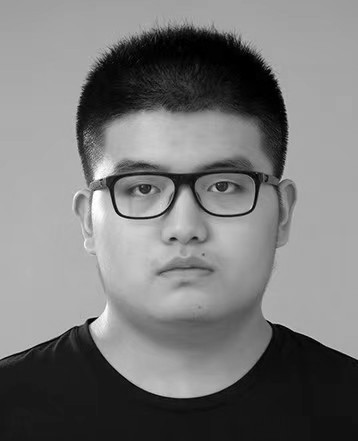
\includegraphics[width=1in,height=1.25in,clip,keepaspectratio]{zuo_bio}}]{Zewen Zuo}
  received the B.Eng. degrees in transportation planning and management from Southeast University, Nanjing, China, in 2020. He is currently pursuing the B.S. degree with the Jiangsu Province Collaborative Innovation Center of Modern Urban Traffic Technologies, School of Transportation. His research interests include traffic flow theory, intelligent transportation systems, and microscopic simualtion.
\end{IEEEbiography}

% biography section
% 
% If you have an EPS/PDF photo (graphicx package needed) extra braces are
% needed around the contents of the optional argument to biography to prevent
% the LaTeX parser from getting confused when it sees the complicated
% \includegraphics command within an optional argument. (You could create
% your own custom macro containing the \includegraphics command to make things
% simpler here.)
%\begin{IEEEbiography}[{\includegraphics[width=1in,height=1.25in,clip,keepaspectratio]{mshell}}]{Michael Shell}
% or if you just want to reserve a space for a photo:

% \begin{IEEEbiography}{Michael Shell}
% Biography text here.
% \end{IEEEbiography}

% % if you will not have a photo at all:
% \begin{IEEEbiographynophoto}{John Doe}
% Biography text here.
% \end{IEEEbiographynophoto}

% insert where needed to balance the two columns on the last page with
% biographies
%\newpage

% \begin{IEEEbiographynophoto}{Jane Doe}
% Biography text here.
% \end{IEEEbiographynophoto}

% You can push biographies down or up by placing
% a \vfill before or after them. The appropriate
% use of \vfill depends on what kind of text is
% on the last page and whether or not the columns
% are being equalized.

%\vfill

% Can be used to pull up biographies so that the bottom of the last one
% is flush with the other column.
%\enlargethispage{-5in}



% that's all folks
\end{document}


